\documentclass[11pt, oneside, onecolumn]{book}
\usepackage{datetime}
\usepackage[utf8]{inputenc}
\usepackage[a4paper, total={6in, 9in}]{geometry}
\usepackage{braket}
\usepackage{xcolor}
\usepackage{amsmath}
\usepackage{amsfonts}
\usepackage{amsthm}
\usepackage{amssymb}
%\usepackage[ocgcolorlinks]{hyperref}
\usepackage{hyperref}
%\usepackage{hyperref,xcolor}
%\usepackage[ocgcolorlinks]{ocgx2}
\usepackage{cleveref}
\usepackage{graphicx}
\usepackage{svg}
\usepackage{float}
\usepackage{tikz}
\usetikzlibrary{patterns, shapes.arrows}
\usepackage{adjustbox}
%\usepackage{tikz-network}
\usepackage{tkz-graph}
\usepackage{tkz-berge}
\usepackage[linesnumbered]{algorithm2e}
\usepackage{multicol}
\usepackage[backend=biber,style=alphabetic,sorting=ynt]{biblatex}
%\usepackage{xcolor}
%\usepackage{tkz-berge}
%\usepackage{tkz-graph}
\usepackage{pgfplots}
\usepackage{sagetex}
\usepackage{setspace}
\usepackage{etoc}
%\usepackage{wrapfig}
\usepackage{pgfgantt}
\DeclareUnicodeCharacter{2212}{−}
\usepgfplotslibrary{groupplots,dateplot}
\pgfplotsset{compat=newest}

\newtheorem{theorem}{Theorem}
\newtheorem{definition}{Definition}
\newtheorem{example}{Example}
\newtheorem{claim}{Claim}
\newtheorem{fact}{Fact}
\newtheorem{remark}{Remark}
\newtheorem*{theorem*}{Theorem}
\newtheorem{lemma}{Lemma}
\crefname{lemma}{Lemma}{Lemmas}
\hypersetup{colorlinks=true}
% , allcolors=blue,allbordercolors=blue,pdfborderstyle={0 0 1}}
%\hypersetup{pdfborder={2 2 2}}
% pdfpagemode=FullScreen,
% backref 

\newtheorem{problem}{Problem}
\crefname{problem}{Problem}{Problems}

\DeclareMathOperator{\Ima}{Im}


\usetikzlibrary{positioning}
\addbibresource{./sample.bib} 


\begin{document}
\newcommand{\commentt}[1]{\textcolor{blue}{ \textbf{[COMMENT]} #1}}
\newcommand{\ctt}[1]{\commentt{#1}}
\newcommand{\prb}[1]{ \mathbf{Pr} \left[ #1 \right]}
\newcommand{\prbm}[2]{ \mathbf{Pr}_{ #2 }\left[ #1 \right]}
\newcommand{\prbc}[3]{ \mathbf{Pr}_{ #2 }\left[ #1 \right | #3]}
\newcommand{\prbcprb}[3]{ \prbc{#2}{#1}{#3} \cdot \prb{#3} } 
\newcommand{\expp}[1]{ \mathbf{E} \left[ {#1} \right]}
\newcommand{\onotation}[1]{\(\mathcal{O} \left( {#1}  \right) \)}
\newcommand{\ona}[1]{\onotation{#1}}
\newcommand{\PSI}{{\ket{\psi}}}
\newcommand{\xij} { X_{ij} } 
\DeclareMathOperator{\Ima}{Im}
%\newcommand{\LESn}{\ket{\psi_n}}
%\newcommand{\LESa}{\ket{\phi_n}}
%\newcommand{\LESs}{\frac{1}{\sqrt{n}}\sum_{i}{\ket{\left(0^{i}10^{n-i}\right)^{n}}}}
%\newcommand{\Hn}{\mathcal{H}_{n}}
%\newcommand{\Ep}{\frac{1}{\sqrt{2^n}}\sum^{2^n}_{x}{ \ket{xx}}}
%\newcommand{\HON}{\ket{\psi_{\text{honest}}}}
%\newcommand{\Lemma}{\paragraph{Lemma.}}
\newcommand{\Cpa}{[n, \rho n, \delta n]}
%\setlength{\columnsep}{0.6cm}
\newcommand{\Jvv}{ \bar{J_{v}} } 
\newcommand{\Cvv}{ \tilde{C_{v}} } 

\newcommand{\Gz}{ G_{z}^{\delta} } 
\newcommand{ \Tann } {  \mathcal{T}\left( G, C_0 \right) }
\newcommand{\ireducable}{ireducable \hyperref[ire]{[\ref{ire}]} }
\newcommand{\cutUU}{E(U_{-1} \bigcup U_{+1} ,U)} 
\newcommand{\wcutUU}{w\left( E(U_{-1} \bigcup U_{+1} ,U)  \right)}
\newcommand{\testgo}{  \mathcal{T}\left(J, q , C_{0}\right) } 

\newcommand{\duC}{\left( C_{A}^{\perp}\otimes C_{B}^{\perp} \right)^{\perp}}
\newcommand{\duduC}{\left( C_{A}\otimes C_{B}\right)^{\perp}}
  




\begin{titlepage}
    \begin{center}
        \vspace*{1cm}
        
        
\includegraphics[width=0.15\textwidth]{huji_logo_notext.pdf}\\
        The Hebrew University of Jerusalem\\
        The Rachel and Selim Benin School of Computer Science and Engineering
        
        \vspace{2cm}
        
        {\Large \textbf{Thesis Title}}
        
        \vspace{1cm}
        \selectlanguage{hebrew}
        {\Large שם העבודה}
        \selectlanguage{english}
        
        \vspace{1.5cm}
        
        \textbf{Author's Name}
        
        \vspace{1cm}
        
        Thesis submitted in partial fulfillment of the requirements\\for the Master of Sciences degree\\
        in Computer Science
        
        \vspace{1cm}
        
        Under the supervision of \textbf{Prof./Dr.~Supervisor's Name}
        
        \vfill
        
        \textbf{Month year}
    \end{center}
\end{titlepage}
%\onehalfspacing
%\title{Understanding Quantumness And Testability.} 
%\author{David Ponarovsky}
\mainmatter


%\maketitle
\input{sageutil.py}
%
\abstract{We propose an alternative simple construction of good LTC codes. In contrast to previews, constructions made by \cite{Dinur}, \cite{leverrier2022quantum} and \cite{Pavel}, our construction doesn't require spicel properties of the small codes, such as $w$-robustness and $p$-resistance for puncturing.  
} 



\tableofcontents
\listoffigures

% \section{Preambles}

Localy Testable Codes, or LTC, are error correction codes such that verfining a uinformly random cchoosen check, would be enough to detect any error with probability proportional to it's size. Bisdes the clear computional adventage they offer, they took roles at the eriler PCP proofs.  
  In this work, we propose a new construction for good LTC codes, which also have a good testability parameter. In the sense   Our proof also indirectly answers the following question. Why most of the good LDPC codes are known to be bad in terms of detecting errors? In other words, It seems that for most of them, there exist strings that are very far from being in the code and, meanwhile, fail to satisfy only a small number of restrictions.
  While the previous LDPC constructions focused on ensuring that the yielded code would have a good rate and distance parameters, our construction enforces the restrictions collection to have a nontrivial fraction of degeneration. That is, removing a single restriction will not change the code, as any restriction is linearly dependent on the others.



\chapter{Introduction}

\chapter{Codes}
  \section{Introduction}
  \section{Introduction.}
.. bla bla bla.. bla bla ..     
\definition[General Entanglement State]{ We say that $\PSI$ is general entanglement \label{def:gEnt} if .. }

\definition[Local-Measure-Circuit] { We say that a quantum circuit $C$ is a local measure circuit \label{def:lmc} if it's can be described as a decomposition of poly classical circuit and a constant depth quantum circuit which contains only 1-qubit gates and measurements. 

We would think about local measure circuits as chip circuits. }

\definition[$p_{0}-\Delta$ Fault Tolerance Circuit]{ We say that $\mathcal{C}$ is $p_{0}-\Delta$ fault tolerance \label{def:gft} presentation of abstract circuit $C$ if there exists a local measure circuit $C_{0}$ \ref{lmc} such it's grunted that for noise $p < p_{0}$ $\mathcal{C}$ compute $C$ w.h.p,
And in addition, if $p \in \left( p_{0}, p_{0} + \varepsilon \right)$ then by applying a $C_{0}$ on $\mathcal{C}$ output yields a general entanglement state \label{def:gEnt}}       

\ctt{We would like to add a complexity parameter for the above definition, for example, ``a general entanglement state over more than $\frac{1}{5}$ of the qubits.}  

  %Linear Error Correction Codes, 
  \subsection{Notations, Definitions, And Our Contribution}
  Here we focus only on linear binary codes, which one could think about as linear subspaces of $\mathbb{F}_{2}^{n}$. A common way to measure resilience is to ask how many bits an evil entity needs to flip such that the corrupted vector will be closer to another vector in that space than the original one. Those ideas were formulated by Hamming \cite{Hamming}, who presented the following definitions. 
  \begin{definition} \label{bi-code} Let $n \in \mathbb{N}$ and $\rho, \delta\in \left( 0,1 \right)$. We say that $C$ is a \textbf{binary linear code} with parameters $[n, \rho n, \delta n]$. If $C$ is a subspace of $\mathbb{F}_{2}^{n}$, and the dimension of $C$ is at least $\rho n$. In addition, we call the vectors belong to $C$ \textit{codewords} and define the distance of $C$ to be the minimal number of different bits between any codewords pair of $C$.   
  \end{definition}
  From now on, we will use the term code to refer to linear binary codes, as we don't deal with any other types of codes. Also, even though it is customary to use the above parameters to analyze codes, we will use their percent forms called the relative distance and the rate of code, matching $\delta$ and $\rho$ correspondingly.     
  \begin{definition} \label{family} A \textbf{family of codes} is an infinite series of codes. Additionally, suppose the rates and relative distances converge into constant values $\rho,\delta$. In that case, we abuse the notation and call that family of codes a code with $[n, \rho n, \delta n]$ for fixed $\rho, \delta\in [ 0,1 )$, and infinite integers $n \in \mathbb{N}$.     
  \end{definition}
  Notice that the above definition contains codes with parameters attending to zero. From a practical view, it means that either we send too many bits, more than a constant amount, on each bit in the original message. Or that for big enough $n$, adversarial, limited to changing only a constant fraction of the bits, could disrupt the transmission. That distinction raises the definition of good codes.

  \begin{definition} \label{good-code} We will say that a family of codes is a \textbf{good code} if its parameters converge into positive values. 
  \end{definition}

  \ifdefined\LDPCLTC
    Apart from distance and rate here, we interest also that the checking process will be robust. In particular,  we wish that against significant errors, forgetting to perform a single check will sabotage the entire computation only with a tiny probability.  
  \begin{definition} \label{LTC} Consider a code $C$  a string $x$, and denote by $\xi\left( x \right)$ the fraction of the checks in which $x$ fails. $C$ will be called a \textbf{local-testability $f\left( n \right)$} If there exists $\kappa > 0$ such that 
  \begin{equation*}
    \begin{split}
      \frac{d\left( x, C \right)}{n} \le \kappa \cdot  \xi\left( x \right) f\left( n \right)
    \end{split}
  \end{equation*}
\end{definition}
 
 %
\fi

  
\ifdefined\LDPCLTC
  Now, we are ready to formulate our contribution. 

  Nowadays, we are aware of a wide range of constructions yield good codes, including the expander codes of Sipser and Spilman \cite{ExpanderCodes} and the LTC codes of Dinur \cite{Dinur}, \cite{Pavel}, \cite{leverrier2022quantum}. Thus if a decade ago, the main question was the existence of a good code and its construction, now, and particularly in this work, we concentrate on getting a deep understanding of what makes those constructions work. By utilizing those insights, we succussed in achieving significantly simpler construction. Our results: 

 \begin{theorem*}[Theorem 1] There exist a constant $\alpha > 0$ and an infinte family of Tanner Codes $C = \Tann$ such that any ireducable codeword $x$ of a coresponding disagreement code $x \in C_{\oplus}$ at length $n$, weight at least $\alpha n$. \end{theorem*}

\begin{theorem*}[Theorem 1+] There exist a constant $\alpha > 0 $ and infinite familiy of codes which satesfies Theroem 1 and also good.
  \end{theorem*}



\fi

  \subsection{Singleton Bound}  
  To get a feeling of the behavior of the distance-rate trade-of, Let us consider the following two codes; each demonstrates a different extreme case. First, define the repetition code $C_{r} \subset \mathbb{F}_{2}^{n \cdot r}$, In which, for a fixed integer $r$, any bit of the original string is duplicated $r$ times. Second, consider the parity check code $C_{p} \subset \mathbb{F}_{2}^{n+1}$, in which its codewords are only the vectors with even parity. Let us analyze the repetition code. Clearly, any two $n$-bits different messages must have at least a single different bit. Therefore their corresponding encoded codewords have to differ in at least $r$ bits. Hence, by scaling $r$, one could achieve a higher distance as he wishes. Sadly the rate of the code decays as $n/nr = 1/r$. In contrast, the parity check code adds only a single extra bit for the original message. Therefore scaling $n$ gives a family which has a rate attends to $\rho \rightarrow 1$. However, flipping any two different bits of a valid codeword is conversing the parity and, as a result, leads to another valid codeword.

  To summarize the above, we have that, using a simple construction, one could construct the codes $[r, 1, r]$, $[r, r-1, 2]$. Each has a single perfect parameter, while the other decays to the worst.\ifdefined\LDPCLTC In the next section, we will review the Singleton bound, which states that for any code (not necessarily good), there must be a zero-sum game between the relative distance and the rate.
\fi % 

  Besides being the first bound, Singleton bound demonstrates how one could get results by using relatively simple elementary arguments. It is also engaging to ask why the proof yields a bound that, empirically, seems far from being tight.
  \begin{theorem*}[Singleton Bound.]\label{theorem*:Sing}  For any linear code with parameter $[n,k,d]$, the following inequality holds:
  \begin{equation*}
    k+ d \le n + 1
  \end{equation*} 
  \end{theorem*}

\begin{proof} Since any two codewords of $C$ differ by at least $d$ coordinates, we know that by ignoring the first $d-1$ coordinate of any vector, we obtain a new code with one-to-one corresponding to the original code. In other words, we have found a new code with the same dimension embedded in $\mathbb{F}_{2}^{n-d+1}$. Combine the fact that dimension is, at most, the dimension of the container space, we get that:  
  \begin{equation*}
    \begin{split}
      \dim C &= 2^{k} \le 2^{n-d+1} \Rightarrow k+d \le n + 1
    \end{split}
  \end{equation*}
\end{proof}

It is also well known that the only binary codes that reach the bound are: $[n,1,n]$, $[n,n-1,2]$,$[n,n,1]$ \cite{eczoo_mds}. In particular, there are no good binary codes that obtain equality(And no binary code which get close to the equality exits). Let's review the polynomial code family \cite{Reed1960PolynomialCO}, which is a code over none binary field that achieve the Singleton Bound. 

\ifdefined\LDPCLTC
\subsection{Polynomial Code.} Consider the field $\mathbb{F}_{m}$ for an arbitrary prime power $m=q^{l}$ greater than $n$. The polynomial codes relay on the fact that any two different polynomials in the ring $\mathbb{F}_{m}\left[ x \right]$ at degree at most $d$ different by at least $m - d + 1$ points. For example consider a polynomials pair at degree 1, namely two linear straight lines. If they are not identical than they have at most single intersection point, and the disagree on each of the $n-1$ remaining points.  

So by define the code to be the subspace contains all the polynomials at degree at most $d$, in such way that any codeword is an image of such polynomail encoded by $n$ numbers, one can garntee a lower bound on the code's distance. Formally we define:     
\begin{definition}[Polynomial Code. \cite{Reed1960PolynomialCO}]
  Fix $m > n $ to be a prime power and let $a_{0},a_{1},a_{2},\ldots a_{n}$ distinct points of the field $\mathbb{F}_{m} = R$  and define the code $C \subset R $ as follows:  
  \begin{equation*}
    \begin{split}
      C = \left\{p\left(a_{0}\right),p\left(a_{1}\right),p\left(a_{2}\right),\cdots p\left(a_{n}\right) : p \text{ is polynomial at degree at most } d \right\}
    \end{split}
  \end{equation*}
\end{definition}
Observe that $C$ is a linear code at length $n$ over the aleph-bet $\mathbb{F}_{m}$. The following Lemma states the realtion between the maximal degree of the polynomials and the properites of the code.   
\begin{lemma}
  Fix the degree of the polynomial code to be at most $d$. Then the parameters of the code are $[n,d + 1, n - d]$.  
  \label{polycode}
\end{lemma}
\begin{proof}
  The dimension of the code equals to the dimension of the polynomials space at degree at most $d$ which is spanned by the monomial base $e_{0}, e_{1}, e_{2} ... e_{d} = 1, x ... x^{d}$ and therefore is $d+1$. In addition suppose that $f,g$ are different polynomials i.e $f\neq g$.

  Hence $h = f-g$ is a non-$0$ polynomial at degree at most $d$ and therefore has at most $d$ roots. Namely at most $d$ points in which $f$ equals $g$ and at least $n-d$ in which they disagree. Put in another way the distance between any two different codewords of the code is at least $n-d$.  
\end{proof}
\begin{sagesilent}
R.<t> = PowerSeriesRing(GF(17));
polyf = (t-1) * (t-2)
polyff = facotr(polyf)
polyg = (t-1) * (t-4)
f(x) = (x-1) * (x-2)
g(x) = (x-1) * (x-4)
pplot_t = finate_poly_plot(f)
pplot_t2 = finate_poly_plot(g)
\end{sagesilent}
\begin{figure}[H]
    \sageplot{ pplot_t + pplot_t2 }
  \caption{The plot presents the extension of the polynomials \sage{polyf} and \sage{polyg} in the filed $\mathbb{F}_{17}$.  }
  \label{fig:polyexample}

\end{figure}

\begin{fact} \label{fact:poly}
  Given $d+1$ points, there is a unique polynomial at degree at most $d$ that pass through all those points. Nevertheless, there is an algorithm $G$ that takes those points as input and outputs the corresponding polynomial.   
\end{fact}

\begin{lemma}[Testability Of Polynomail Code.] The polynomial code is $\left(d \cdot \log\left( n \right), \varepsilon  \right) $ testable.   

\end{lemma}
\begin{proof}
Denote by $f \in \mathbb{F}_{m}^{n}$ a codeword candidate and consider the following test. First, choose uniformly at random $d+1$ points $x_{1}, x_{2}, x_{3}, ... x_{d+1}$ and use $G$ to output a polynomial that agree on that points, denote it by $G\left( f \right)$. Then uniformly choose an additional point, return \textbf{True} if $G\left( f \right)(x_{d+2}) = f\left( x_{d+2} \right)$ and \textbf{False} otherwise.   

  Now, observe that if $f\in C$ then by ~\cref{fact:poly} we have that $G\left( f \right) = f$. In particular $G\left( f \right)(x_{d+2}) = f\left( x_{d+2} \right)$, Namely the test validate a codeword with probability $1$.   

  Now consider the case that $f \neq C$. And observes that $1 - \frac{1}{n} d\left( f, C \right)$ is the maximal fraction $\eta$ such that there exists a polynomial agree with $f$ on at least $\eta n$ points. Then we have:

  \begin{equation*}
    \begin{split}
      \eta & \le \mathbf{Pr}_{x_{1}, x_{2} ... x_{d} \sim_{U}, x_{d+1}\sim \mathbb{F}_{}}\left[ (Gf)(x) = f(x) \right] \\ & \le \prb{ (Gf)(x) = f(x)} \le \varepsilon \\
       1 - \eta & \ge 1 - \varepsilon 
    \end{split}
  \end{equation*}
\end{proof}

  
%+  point(p_list2, size=1, color='green')
 
\fi

Next, we will review Tanner's construction, that in addition to being a critical element to our proof, also serves as an example of how one can construct a code with arbitrary length and positive rate.

\subsection{Tanner Code}
The constructions require two main ingredients: a graph $\Gamma$, and for simplicity, we will restrict ourselves to a $\Delta$ regular graph, Yet notice that the following could be generalize straightforwardly for graphs with degree at most $\Delta$. The second ingredients is a ;small' code $C_{0}$ at length equals the graph's regularity, namely $C_{0} = [\Delta,\rho\Delta, \delta\Delta]$. We can think about any bit string at length $\Delta$ as an assignment over the edges of the graph. Furthermore, for every vertex $v \in \Gamma$, we will call the bit string, which is set on its edges, the local view of $v$. Then we can define, \cite{Tanner}:
  \begin{definition}  Let $ C = \mathcal{T}\left( \Gamma, C_{0} \right)$  be all the codewords which, for any vertex $v\in \Gamma$, the local view of $v$ is a codeword of $C_{0}$. We say that $C$ is a \textbf{Tanner code}\label{Tan} of $\Gamma, C_{0}$. Notice that if $C_{0}$ is a binary linear code, So $C$ is.  
  \end{definition}
  \begin{example}
Consider the Petersen graph $\Gamma$, which is a regular graph with degree $3$. Let $C_{0}$ be the set of all words with even parity. It follows that $C_{0}$ contains all even-length binary strings of length $3$: $000$, $110$, $101$, and $011$. However, the size of $\mathcal{T}(\Gamma, C_{0})$ is significantly larger, as shown in Figure \cref{fig:pet}. Specifically, any rotation of the inner and outer cycles simultaneously gives rise to another valid codeword, so any assignments that are not invariant under these rotations would produce five additional valid codewords.

  \end{example}
\begin{sagesilent}
   
  
ggs = peter_graphs()
ff = cycle_graph()
for gg in ggs:
  gg.set_latex_options(
          edge_label_sloped = False,
          edge_labels=True,
          edge_thickness=0.005,
          vertex_labels=False,
          vertex_size= 0.01,
          format='dot2tex',
          prog='crico',
          graphic_size=(7,7),
          edge_fills=False,
      )
ff.set_latex_options(
          edge_label_sloped = False,
          edge_labels=True,
          edge_thickness=0.005,
          vertex_labels=False,
          vertex_size= 0.01,
          format='dot2tex',
          prog='crico',
          graphic_size=(30,8),
          edge_fills=False,
      )
 
ops = [ gg.latex_options() for gg in ggs ] 
ops2 = ff.latex_options()

graphs_tex =  ' \ \ \ '.join([  str(op.tkz_picture())  for op in ops[:3 ]])
graphs_tex_2 =  ' \ \ \ '.join([  str(op.tkz_picture())  for op in ops[3:]])
graphs_tex_ff  = str(ops2.tkz_picture())
\end{sagesilent}

\begin{center}
  \begin{figure}[H]
    \scalebox{0.5}{
      \sagestr{graphs_tex}
   }
  \caption{Peterson Graph.} 
  \label{fig:pet}
\end{figure}
\end{center}

%\begin{center}
%  \begin{figure}[H]
%    \scalebox{0.5}{
%      \sagestr{graphs_tex_2}
%   }
%  %\caption{Peterson Graph.} 
%  \label{fig:pet2}
%\end{figure}
%\end{center}
  %It's also worth mentioning that the first construction of good classical codes, due to Sipser and Shpilman, are Tanner codes over expanders graphs \cite{ExpanderCodes}.
  \begin{lemma}
\label{tanrate} Tanner codes have a rate of at least $2\rho - 1$.
\end{lemma}
  \begin{proof}  The dimension of the subspace is bounded by the dimension of the container minus the number of restrictions. So assuming non-degeneration of the small code restrictions, we have that any vertex count exactly $ \left( 1 - \rho  \right)\Delta $ restrictions. Hence, \begin{equation*}
    \begin{split}
      \dim C & \ge \frac{1}{2}n\Delta - \left( 1-\rho \right)\Delta n = \frac{1}{2}n\Delta\left( 2\rho - 1 \right)  
    \end{split}
  \end{equation*} Clearly, any small code with rate $> \frac{1}{2}$ will yield a code with an asymptotically positive rate \end{proof} 
  %\subsubsection{Positive Rate, Arbitrarily Large Codes.} 
  Based on \cref{tanrate}, we can obtain a recipe for constructing codes with a almost non-vanishing rate for arbitrarily large lengths and dimensions. This recipe involves concatenating a series of Tanner codes over complete graphs. To be more precise, we can define a family of codes as follows:
  \begin{equation*}
    \begin{split}
      C_{i+1} & = \mathcal{T}\left( K_{n(C_{i}) + 1}, C_{i} \right) \\
      C_{0} &= \text{ Some simple } \Delta[1, \rho_{0}, \delta_{0}] \text{ code. }
    \end{split}
  \end{equation*}
Where $n(C_i)$ represents the code length of the $i$th code. Repeating the process described above $\log_{\Delta}^{*}(n)$ times allows us to extend the initial code $\Delta[1,\rho_{0}]$ to $n[1, \sim 2\rho^{\log_{\Delta}^{*}(n)}]$. Interestingly, any family of finite groups generated by a constant-size generator set can define a family of codes by utilizing their Cayley graphs as a basis for Tanner codes.

  Once we have seen that Tanner codes enable us to achieve rates, the next natural question to ask is about the distance of the codes. Achieving a linear distance requires a little bit more from the graphs, but to understand this idea better, let us return to the repetition code. For instance, the repetition code can be presented as a Tanner code over the cycle graph.  

  \begin{example}
    In this representation, each vertex checks if the bits on its edges are equal. A valid codeword is an assignment in which all the bits are equal, since otherwise, there would be an edge with no supporting vertex. An illustration of a legal assignment is provided in \cref{fig:cyc}.\end{example} 

% \begin{center}
%  \begin{figure}[H]
%    \scalebox{0.5}{
 %     \sagestr{graphs_tex_ff}
%    }
%  \caption{Cycle Graph.} 
%  \label{fig:cyc}
%\end{figure}
%\end{center}

Recall that the distance of a linear code is the minimal weight of the non-zero codewords. Consider a codeword $c \in C$ and group the vertices by four sets $V_i$ such that $V_i$ is the set of vertices that see $i \in \{0,1\}^{2}$. Since $c \in C$, we have that $|V_{10}|=|V_{01}| = 0$. Additionally, any vertex in $V_{00}$ is not connected to $V_{11}$, which gives us two possible cases: either all the vertices in $V_{11}$ are isolated, or the graph is not connected. Hence, the distance of the code is equal to $\frac{1}{2}\sum{|V_{i}|\cdot |i|} = \frac{1}{2}2 \cdot n = n$.

Analyzing the repetition code gives a clue of how, in certain cases, one might prove a lower bound on the code distance. We would like to say that, if the weight of the code word is below the distance, then it is must be that is at least one vertex see non trivial local view which is not a codeword in $C_{0}$. Put it differently, we can't spread a small weight codeword over $\{V_{i}\}$, defined above, without to expanse into subsets corresponds to low $|i|$. Next we are going to present the Expander codes, which are Tanner codes constructed by graph with good algebraic expansion.   

%Note that for any $S\subset V$ and $ S \neq V $, 

%But on the other hand any vertex in $V_{00}$ can't be connected to $V_{11}$, Thus we obtain that either all the vertices in $V_{11}$ tr that the graph is not connected. The distance of the code is $\frac{1}{2}\sum{|V_{i}|\cdot |i|} = \frac{1}{2}2 \cdot n = n$.      
% The idea  

  \subsection{Expander Codes}
  We saw how a graph could give us arbitrarily long codes with a positive rate. We will show, Sipser's result \cite{ExpanderCodes} that if the graph is also an expander, we can guarantee a positive relative distance. 
  \begin{definition} Denote by $\lambda$ the second eigenvalue of the adjacency matrix of the $\Delta$-regular graph. For our uses, it will be satisfied to define expander as a graph $G = \left( V,E \right)$ such that for any two subsets of vertices $T,S \subset V$, the number of edges between $S$ and $T$ is at most:
  \begin{equation*}
    \begin{split}
      \mid E\left( S,T \right) - \frac{\Delta}{n}|S||T| \mid \le \lambda\sqrt{|S| |T|} 
    \end{split}
  \end{equation*}
\end{definition}
This bound is known as the Expander Mixining Lemma. We refer the reader to \cite{hoory2006expander} for more deatilied survery. 
  \begin{theorem*} Theorem, let $C$ be the Tanner Code defined by the small code $C_{0} = [\Delta,\delta\Delta, \rho\Delta ]$ such that $\rho \ge \frac{1}{2}$ and the expander graph $G$ such that $\delta\Delta \ge \lambda$. $C$ is a good  LDPC code.
  \end{theorem*}
  \begin{proof} We have already shown that the graph has a positive rate due to the Tunner construction. So it's left to show also the code has a linear distance. Fix a codeword $x \in C$ and denote By $S$ the support of $x$ over the edges. Namely, a vertex $v\in V$ belongs to $S$ if it connects to nonzero edges regarding the assignment by $x$, Assume towards contradiction that $|x| = o\left( n \right)$. And notice that $|S|$ is at most $2|x|$, Then by The Expander Mixining Lemma we have that: 
  \begin{equation*}
    \begin{split}
      \frac{E\left( S,S \right)}{|S|} & \le \frac{\Delta}{n}|S|  + \lambda \\
      & \le_{ n \rightarrow \infty} o\left( 1 \right) + \lambda
    \end{split}
  \end{equation*}

  Namely, for any such sublinear weight string, $x$, the average of nontrivial edges for the vertex is less than $\lambda$. So there must be at least one vertex $v \in S$ that, on his local view, sets a  string at a weight less than $\lambda$. By the definition of $S$, this string cannot be trivial. Combining the fact that any nontrivial codeword of the $C_{0}$ is at weight at least $\delta\Delta$, we get a contradiction to the assumption that $v$ is satisfied, videlicet, $x$ can't be a codeword \end{proof}

  \subsubsection{Setting $C_{0}$ To Be The Polynomial Code.}
  
  \begin{equation*}
    \begin{split}
     \log \Delta \dim C & \ge \frac{1}{2}n\Delta  - \left( 1- \rho  \right) \Delta n = \frac{1}{2}n\Delta\left( 2\rho - 1 \right)  \\
     \Rightarrow  \dim C & \ge \frac{1}{\log \Delta} \frac{1}{2}n\Delta\left( 2\rho - 1 \right)  
    \end{split}
  \end{equation*}


\subsubsection{Note On Quantum Polynomial Code.} 
Let's define the code $C$ such that any state in $C$ is a coset of the polynomials at degree at most $d$ shifted by $x \in \mathbb{F}_{p}$. In other words the codeword associated with $x$ is the state $\ket{\underline{c}} = \sum_{ \substack{ f \in \mathbb{F}_{d}[x] \\  f(0) = 0}}{ \ket{ c + f}} $. The inner product between any $d$-degree polynomial with zero free coefficient is:
\begin{equation*}
  \begin{split}
    \braket{ f | x^{j} } = \sum_{i \le d }{ \braket{a_{i} x^{i} | x^{j}}} = \sum_{i \le d}{ a_{i} \expp{ x^{i}x^{j}   }} =  \sum_{i \le d}{ a_{i } \mathbf{1}_{ i + j =_{n} 0 }}
  \end{split}
\end{equation*}
\ctt{Say some words about the classily testability of the polynomial code, and why for quantum it doesn't work. (The dual space of polynomials of low degree is the subspace of all the polynomials with heigh degree.)}



\printbibliography[heading=subbibliography]


\chapter{Locally Testable Codes.}
  Apart from distance and rate here, we interest also that the checking process will be robust. In particular,  we wish that against significant errors, forgetting to perform a single check will sabotage the entire computation only with a tiny probability.  
  \begin{definition} \label{LTC} Consider a code $C$  a string $x$, and denote by $\xi\left( x \right)$ the fraction of the checks in which $x$ fails. $C$ will be called a \textbf{local-testability $f\left( n \right)$} If there exists $\kappa > 0$ such that 
  \begin{equation*}
    \begin{split}
      \frac{d\left( x, C \right)}{n} \le \kappa \cdot  \xi\left( x \right) f\left( n \right)
    \end{split}
  \end{equation*}
\end{definition}
 

\subsection{Polynomial Code.} Consider the field $\mathbb{F}_{m}$ for an arbitrary prime power $m=q^{l}$ greater than $n$. The polynomial codes relay on the fact that any two different polynomials in the ring $\mathbb{F}_{m}\left[ x \right]$ at degree at most $d$ different by at least $m - d + 1$ points. For example consider a polynomials pair at degree 1, namely two linear straight lines. If they are not identical than they have at most single intersection point, and the disagree on each of the $n-1$ remaining points.  

So by define the code to be the subspace contains all the polynomials at degree at most $d$, in such way that any codeword is an image of such polynomail encoded by $n$ numbers, one can garntee a lower bound on the code's distance. Formally we define:     
\begin{definition}[Polynomial Code. \cite{Reed1960PolynomialCO}]
  Fix $m > n $ to be a prime power and let $a_{0},a_{1},a_{2},\ldots a_{n}$ distinct points of the field $\mathbb{F}_{m} = R$  and define the code $C \subset R $ as follows:  
  \begin{equation*}
    \begin{split}
      C = \left\{p\left(a_{0}\right),p\left(a_{1}\right),p\left(a_{2}\right),\cdots p\left(a_{n}\right) : p \text{ is polynomial at degree at most } d \right\}
    \end{split}
  \end{equation*}
\end{definition}
Observe that $C$ is a linear code at length $n$ over the aleph-bet $\mathbb{F}_{m}$. The following Lemma states the realtion between the maximal degree of the polynomials and the properites of the code.   
\begin{lemma}
  Fix the degree of the polynomial code to be at most $d$. Then the parameters of the code are $[n,d + 1, n - d]$.  
  \label{polycode}
\end{lemma}
\begin{proof}
  The dimension of the code equals to the dimension of the polynomials space at degree at most $d$ which is spanned by the monomial base $e_{0}, e_{1}, e_{2} ... e_{d} = 1, x ... x^{d}$ and therefore is $d+1$. In addition suppose that $f,g$ are different polynomials i.e $f\neq g$.

  Hence $h = f-g$ is a non-$0$ polynomial at degree at most $d$ and therefore has at most $d$ roots. Namely at most $d$ points in which $f$ equals $g$ and at least $n-d$ in which they disagree. Put in another way the distance between any two different codewords of the code is at least $n-d$.  
\end{proof}
\begin{sagesilent}
R.<t> = PowerSeriesRing(GF(17));
polyf = (t-1) * (t-2)
polyff = facotr(polyf)
polyg = (t-1) * (t-4)
f(x) = (x-1) * (x-2)
g(x) = (x-1) * (x-4)
pplot_t = finate_poly_plot(f)
pplot_t2 = finate_poly_plot(g)
\end{sagesilent}
\begin{figure}[H]
    \sageplot{ pplot_t + pplot_t2 }
  \caption{The plot presents the extension of the polynomials \sage{polyf} and \sage{polyg} in the filed $\mathbb{F}_{17}$.  }
  \label{fig:polyexample}

\end{figure}

\begin{fact} \label{fact:poly}
  Given $d+1$ points, there is a unique polynomial at degree at most $d$ that pass through all those points. Nevertheless, there is an algorithm $G$ that takes those points as input and outputs the corresponding polynomial.   
\end{fact}

\begin{lemma}[Testability Of Polynomail Code.] The polynomial code is $\left(d \cdot \log\left( n \right), \varepsilon  \right) $ testable.   

\end{lemma}
\begin{proof}
Denote by $f \in \mathbb{F}_{m}^{n}$ a codeword candidate and consider the following test. First, choose uniformly at random $d+1$ points $x_{1}, x_{2}, x_{3}, ... x_{d+1}$ and use $G$ to output a polynomial that agree on that points, denote it by $G\left( f \right)$. Then uniformly choose an additional point, return \textbf{True} if $G\left( f \right)(x_{d+2}) = f\left( x_{d+2} \right)$ and \textbf{False} otherwise.   

  Now, observe that if $f\in C$ then by ~\cref{fact:poly} we have that $G\left( f \right) = f$. In particular $G\left( f \right)(x_{d+2}) = f\left( x_{d+2} \right)$, Namely the test validate a codeword with probability $1$.   

  Now consider the case that $f \neq C$. And observes that $1 - \frac{1}{n} d\left( f, C \right)$ is the maximal fraction $\eta$ such that there exists a polynomial agree with $f$ on at least $\eta n$ points. Then we have:

  \begin{equation*}
    \begin{split}
      \eta & \le \mathbf{Pr}_{x_{1}, x_{2} ... x_{d} \sim_{U}, x_{d+1}\sim \mathbb{F}_{}}\left[ (Gf)(x) = f(x) \right] \\ & \le \prb{ (Gf)(x) = f(x)} \le \varepsilon \\
       1 - \eta & \ge 1 - \varepsilon 
    \end{split}
  \end{equation*}
\end{proof}

  
%+  point(p_list2, size=1, color='green')


%\printbibliography[heading=subbibliography]

\chapter{Quantum Error Correction Codes.}
\section{Introduction.}
It's widely believed that quantum machines have a significant advantage over the classical in the range of computational tasks\cite{grover1996fast}, \cite{ahuja1999quantum}. Simple algorithms could be interpreted as the quantum version of scanning all the options, cutting the running time by the square root of the classical magnitude. 

Nevertheless, Shore has shown a polynomial depth quantum circuit that solves the hidden abelian subgroup \cite{Shor_1997}, which is considered a breakthrough, as it made the computer science community believe that a quantum computer might offer an exponential advantage.

Yet, even though there is a consensus about the superiority of ideal quantum computation model, it is still unclear whether implementing such a machine in the presence of noise is feasible.   
Still, just pointing on the existence of noise is not powerful enough to cancel the feasibility of computation. Evidence of this is that classical computers also suffer from a certain rate of faults. Thus, to fully understand the hardness, let us compare two main reasons that made it realize a hard task. 
First is the magnitude of the error rate, classical computers also have errors, and sometimes we witness system failures (blue screen, for example). The error rate of modern computers is so low that the probability for error to propagate stays negligible even if the length of the computation is polynomial in the scale of what is considered reasonable input size. It's worth mentioning that in exascale computing when supercomputers perform around $10^{18}$ operations per second, It is hard to miss the faults. In quantum, we become aware of their existence much earlier.      

The second difference, which is a tricky point, is that quantum states are sensitive to additional types of error. Along with the chance for bit-flip error, a quantum state might also change its phase. For example, consider the initial state $\ket{+} = \frac{1}{\sqrt{2}}\left( \ket{0} + \ket{1} \right)$, and suppose that due to noise the state transformed into $\frac{1}{\sqrt{4}}\left( \sqrt{3}\ket{0} + \ket{1} \right)$. While classical circuits are blind to such faults. Namely, their run would stay identical as no error occurs. Quantum circuits usually would affect and might fail. Furthermore, when planning a decoder for quantum error correction codes, If one is willing to use a classical code to defend against phase flips, he has to ensure that the decoding doesn't cause bit-flip errors. 


\ifdefined\qnoise
  \begin{document}
\fi
\section{Quantum Noise.} 
\begin{definition}[Bit and pahse flip.] \label{def:bphf}  
  Consider a quantum state $\ket{\psi}$ encoded in the computation base. We will say that a \textit{bit-flip} occurs in a scenario the operator Pauli $X$ is applied on one of our state's qubits. The bit-flip event could be considered as exactly as the standard bit-flip error in the classical regime. Similarly, \textit{phase-flip} occurs when the Pauli $Z$ is applied on one of the qubits. 

  \end{definition}

  % Notice that together with the identity $I$, the set $\{I, X \otimes e_{i} , Z \otimes e_{j} \}_{i,j \in [n]}$ span the matrices act on $n$ qubits.  


\ifdefined\qnoise
  \end{document}
\fi
 
However, even though quantum noise is so violent, It was proven that any ideal circuit at polynomial depth could be transformed to a robust circuit at poly-logarithmic cost \cite{aharonov1999faulttolerant}. Or in other words, There is a threshold, If the physicists would provide qubits and a finite gate set that suffers from a rate of noise below that threshold, then $BQP$, the class of polynomial time ideal quantum computation is feasible and could be computed on a realistic machine.                

The basic ingredient in \cite{aharonov1999faulttolerant} was to show the existence of quantum error correction code, such that one can perform all the logic operations in a way that restricts present errors from propagating on. That allows them to separate any operation of the computation into stages; one of them is the operation itself, another one is an error correction stage. That process comes with an additional cost, in both space and time, yet it might decrease the probability that the final state at the end would be faulted. The trade-off between the resource needed to pay and the decreasing rate defines the threshold. And if the balance is positive, then one can repeat in a recursion manner, and after log-log iterations, the failure probability decay to zero. At the same time, the circuit would scale at most poly-logarithmic wide and depth factors.      

Let's return to the repetition code presented in Chapter 2. We would like to have an analog; a first and natural attempt might consider duplicating copies of the state. Unfortunately, copying a general state is not a linear operation and therefore can not be done in the circuit model (and any other believed to be feasible). In particular there is no circuit $U$ which duplicate simultaneity the states $\ket{0}, \ket{1}, \ket{+}, \ket{-}$.

To overcome the issue, Shor came up with the nine-quibt code \cite{Ninequ}, which at first glance might seem a naive straightforward implantation of ``duplication'', but instead uses a clever insight about quantumness in general. Any operation can be seen as a linear (and even unitary) operation over a subspace embedded in large enough dimensions. The encoding is given as follow: 
\begin{equation*}
  \begin{split}
    |\overline{0}\rangle&=\frac{1}{2\sqrt{2}}\left(|000\rangle+|111\rangle\right)^{\otimes3}\\
    |\overline{1}\rangle&=\frac{1}{2\sqrt{2}}\left(|000\rangle-|111\rangle\right)^{\otimes3}~.
  \end{split}
\end{equation*}


For convenient let us use the notation, $\ket{\mathbf{GHZ}^{\pm}} =  \ket{0^{m}} \pm  \ket{1^{m}}$. One can also consider the Shor code over $m^{2}$ qubits which defined as above beside that any logical state contain $m$ product over $m$ qubits, So the state $\ket{\overline{0}}$ over $m^{2}$ qubits can be written as $\ket{\mathbf{GHZ}^{+}}^{m}$. We are now ready to prove a statement regards to the robustness.  

\begin{lemma}
  The Shor code over $9$ qubits enable to correct a single either bit or phase flip.  
\end{lemma}
It is evident that a single bit-flip error can be handled in the same way as in the conventional case. The decoder will check if any of the triples have the same value, and if not, it will correct it by majority. To create a decoder that can also correct a phase-flip error, we need the following statement. In this chapter, we denote the Hadamard gate over $m$ qubits as $H^m$.
\begin{claim}
   $H^{m}\ket{\mathbf{GHZ}^{\pm}} = \sum_{ x \cdot \mathbf{1} =_2 \pm }{\ket{x} }$
\end{claim}

\begin{proof}

  \begin{equation*}
    \begin{split}
      H^{m}\ket{\mathbf{GHZ}^{\pm}} & = H^{m}\ket{0^{m}} \pm  H^{m}\ket{1^{m}} = \sum_{x \in \mathbb{F}_{2}^{m}}{\ket{x}} \pm  \sum_{x \in \mathbb{F}_{2}^{m}}{\left( -1 \right)^{x \cdot \mathbf{1}} \ket{x}} \\ & = \sum_{x \in \mathbb{F}_{2}^{m}}{ \left( 1 \pm \left( -1 \right)^{x \cdot \mathbf{1}}  \right) \ket{x} } =  \sum_{x \cdot \mathbf{1} =_2 \pm }{\ket{x} }
    \end{split}
  \end{equation*}
\end{proof}

Now it is clear how to correct a phase flip. One can apply the Hadamard transform and compute the parity of each triple. By the assumption that only a single phase flip may occur, either all the triples have the same parity or the faulted one has an opposite parity and needs to be corrected. Thus, we obtain an $\left[ \left[ 9,1,3 \right] \right]$ quantum error correction code. Asymptotically, this is an $\left[ \left[ m^{2}, 1, m \right] \right]$ code.

\section{CSS Codes.}

The Shor code is a specific case of the more general CSS (Calderbank-Shor-Steane) code \cite{Calderbank_1996}. A family composed by two binary codes $C_{X}, C_{Z}$ such that $C_{Z}^{\perp} \subset C_{X}$. 

\ifdefined\CSSDOC
\begin{document}
\fi 

\ctt{Add a definition of error weight. fault that spanned by pauli operator of degree at} 

\begin{definition}[CSS Code]
  Let $C_{X}, C_{Z}$ classical linear codes such that $C_{Z}^{\perp} \subset C_{X}$ define the $Q\left( C_{X},C_{Z} \right)$ to be all the code words with following structure:
  \begin{equation*}
    \begin{split}
    \ket { \mathbf{ x } } := \ket { x + C_{Z}^{\perp} } = \frac{1}{\sqrt{C_{Z}^{\perp}}} \sum_{z \in C_{Z}^{\perp}}{ \ket{ x + z }} 
    \end{split}
  \end{equation*}
\end{definition}
Clearly, the codewords are all the codewords in $C_{X}$ which don't belong to $C_{Z}^{\perp}$ and therefore the dimension of the quantum code is $\dim Q\left( C_{X}, C_{Z} \right) = \dim C_{X} - \dim C_{Z^{\perp}} = \dim C_{X} + \dim C_{Z} - n$. Yet, it's not stems immediately how one can correct faults. Next, we are going to repeat the decoding process of the Shor code in the general setting of CSS codes.  
\begin{lemma}
  Let $C_{X},C_{Z}$ classical codes such $Q\left( C_{X},C_{Z} \right)$ is a CSS code. Let $d_{X}$ be the minimal weigh of codeword in $C_{X}$ which is not in $C_{Z}^{\perp}$, and define by the same way $d_{Z}$ to be the minimal weight of codeword in $C_{Z}$ which doesn't belong to $C_{X}^{\perp}$. Then the distance of $Q\left( C_{X},C_{Z} \right)$ equals to $\min{d_{X},d_{Z}}$. Moreover there is a decoder which correct any fault with weight at most $d/2$.       
  \end{lemma}

    \newcommand{\GZZZ}[1]{ \frac{1}{\sqrt{|C_{Z}^{\perp}|}} \sum_{z \in C_{Z}^{\perp}}{ #1 } } 
    \newcommand{\GZZZW}[2]{ \frac{1}{\sqrt{|C_{Z}^{\perp}|}} #2 \sum_{z \in C_{Z}^{\perp}}{ #1 } } 
    \newcommand{\GXXX}[1]{ \frac{1}{\sqrt{|C_{Z}|}} \sum_{z \in C_{Z}}{ #1 } } 
    \newcommand{\GXXXW}[2]{ \frac{1}{\sqrt{|C_{Z}|}} #2 \sum_{z \in C_{Z}}{ #1 } } 

  \begin{proof}
    First let us prove the following claim: 
    \begin{claim}
      Denote by $H^{\otimes n}$ the Hadamard gate over $n$ qubits. Then for any code $C$ it holds that: $  H^{n}\ket{C^{\perp}} = \ket{C} $
          \end{claim}
    \begin{proof}
      \begin{equation*}
        H^{n}\ket{C^{\perp}} = \GZZZ{ H^{n}\ket{z} } = \frac{1}{ \sqrt{ 2^{n}}} \GZZZ{ \sum_{y\in \mathbb{F}_{2}^{n}}{ (-1)^{\braket{z,y}}  \ket{y}}  }
       \end{equation*}
       Notice that $ 2^{n}|C_{Z}^{\perp}| =  |C_{z}| \cdot |C_{Z}^{\perp}| \cdot |C_{Z}^{\perp}|$  
    \end{proof}
    \begin{claim}
      For any $x_{0} \in C_{X}$ and $z_{1}\neq z_{2} \in C_{z}^{\perp}$, $D$ correct $\ket{x+z_{1}+f}$, $\ket{x+z_{2}+f}$ into two different words in $C_{X}$. 
    \end{claim} 
    \begin{proof}
      Suppose not, namely there exists $y \in C_{X}$ such that $D$ correct $\ket{x+z_{1}+f}$, $\ket{x+z_{2}+f}$ into $\ket{y}$. Then we have that for both $i\in \{1,2\}$ it holds that  $d\left( x+z_{i} +f, y \right) \le d\left( C_{Z}^{\perp}/2 \right)$ and therefore $ d\left( x + z_{1} + f, x+z_{2} +f  \right) \le d\left( C_{Z}^{\perp} \right)$. But
      \begin{equation*}
        \begin{split}
            & d\left( x + z_{1} + f, x+z_{2} +f  \right) =  | x + z_{1} + f + x + z_{2} + f | \\
            =  & | z_{1} + z_{2} | = d\left( z_{1},z_{2} \right) > d\left( C_{Z}^{\perp} \right) 
        \end{split}
      \end{equation*}     
      contradiction for the assumption that $z_{1},z_{2} \in C_{Z}^{\perp}$.   
    \end{proof}
    Let $P = X^{f}Z^{e}$ be an error such that $e, f < d/2$ act on the state $\ket{\mathbf{x}}$. Denote by $H_{X}, H_{Z}$ the parity check matrices of $C_{X},C_{Z}$. 
      \begin{equation*}
      \begin{split}
        \ket{\mathbf{x}} &  \mapsto^{P}   \frac{1}{\sqrt{|C_{Z}^{\perp}|}} \sum_{z \in C_{Z}^{\perp}}{ X^{f}Z^{e}\ket{ x + z }} = \frac{1}{\sqrt{|C_{Z}^{\perp}|}} \sum_{z \in C_{Z}^{\perp}}{ (-1)^{\braket{e,f} }Z^{e}\ket{ x + z + f}}\\
        & \mapsto^{H_{X}} \GZZZ{ (-1)^{\braket{e,f} }Z^{e}\ket{ x + z + f} \ket{ H_{X} \left(x + z + f\right) }  } \\ 
        & = \ \ \ \ \ \GZZZ{ (-1)^{\braket{e,f} }Z^{e}\ket{ x + z + f} \ket{ H_{X}f }  }\\
        & \mapsto^{X^{f}} \GZZZ{ Z^{e}\ket{ x + z} \ket{ H_{X}f }  }  \mapsto^{H^{\otimes n}} \GZZZ{  X^{e}H^{\otimes n}\ket{ x + z} } \\
        & = \GZZZ{  X^{e}H^{\otimes n} X^{x} \ket{ z} }  = \GZZZ{  X^{e} Z^{x} H^{\otimes n} \ket{ z} } \\
        & = \GZZZW{ \ket{ z} }{X^{e} Z^{x} H^{\otimes n} }  =  \GXXXW{  \ket{ z} }{ X^{e} Z^{x} } \\
        & =  \GXXXW{   X^{e}\ket{ z} }{ (-1)^{\braket{x,e}} Z^{x}}  =  \GXXXW{   \ket{ z + e} }{ (-1)^{\braket{x,e}} Z^{x}} \\
        & =  \GXXXW{   \ket{ z + e} \ket{ H_{Z}e }}{ (-1)^{\braket{x,e}} Z^{x}} \\
        & \mapsto  \GXXXW{   \ket{ z } \ket{ H_{Z}e }}{ (-1)^{\braket{x,e}} Z^{x}} \mapsto^{H^{n}}  \GZZZW{   \ket{ z }}{ X^{x}}\\ 
        & = \GZZZ{ \ket{z + x}} = \ket{\mathbf{x}}
      \end{split}
    \end{equation*}
  \end{proof}
  
  There is still one big difference between the classic repetition code and the Shor code. While each parity check of the Shor code examines a square root number of qubits, any check of the repetition code touches no more than a constant number of qubits; that is, any check just tests if any two adjacent bits are equal.  That brings us to ask whether the Shors code is really the quantum analogy for the repetition code? 

  For getting an hint before formally presenting a quantum LDPC code, let's take another look on the general structure of the CSS codes. The decoding procedure the proof above teach us an additional point about CSS code, the task of finding a good code quantum code, could be reduce for finding a two classic binary linear codes which their parity check matrices ortogonal to each other. Furthermore, if one is willing to has an qLDPC code, then $H_{X}$ and $H_{Z}$ can't be parity check matrices of good classical code as any column of $H_{z}^{\top}$ is a codeword of $C_{X}$. 
  \begin{equation*}
    \begin{split}
      C_{Z}^{\perp} \subset C_{X} \Rightarrow H_{X}H_{Z}^{\top} = 0 
    \end{split}
  \end{equation*}


\ifdefined\CSSDOC
\end{document}
\fi 


  \section{qLDPC Codes.}
  As exactly as in the classic case, qLDPC codes are codes in which any check act non trivially on at most a constant number of qubits, It was proved that using a good Quantum LDPC code one can achieve a fault tolerance threshold theorem at the cost of only constant overhead\footnote{under the assumption of holding an efficient decoder.} \cite{gottesman2014faulttolerant}. We are now about to embark on a detailed review of the first quantum LDPC code \cite{Dennis_2002}. 

  Recall that one way to present a code is by define the parity check matrix, Consider the $l\times l$ Tours, namely the Cayley graph of the group product  $\mathbb{Z}_{l} \times \mathbb{Z}_{l}$. Associate any coordinate (bit/qubit) with an edge on the Tours. And consider the following two restrictions:

  \begin{enumerate}
    \item Each vertex requires form its local view, the bits lay on its supported edges, To has an even party. We will refer to this type of check as \textit{cross check}. 
    \item Similarly, each face requires the same from its supported edges, but computes the parity in a different (specific) base. That it, the face first rotates the qubits by applying the Hadamard transform on them, and then computes their XOR. Finally, the qubits are rotated back to the computation base. We shall refer to this type of check as \textit{face check}.
  \end{enumerate}

  \begin{center}
    \begin{figure}[H]
  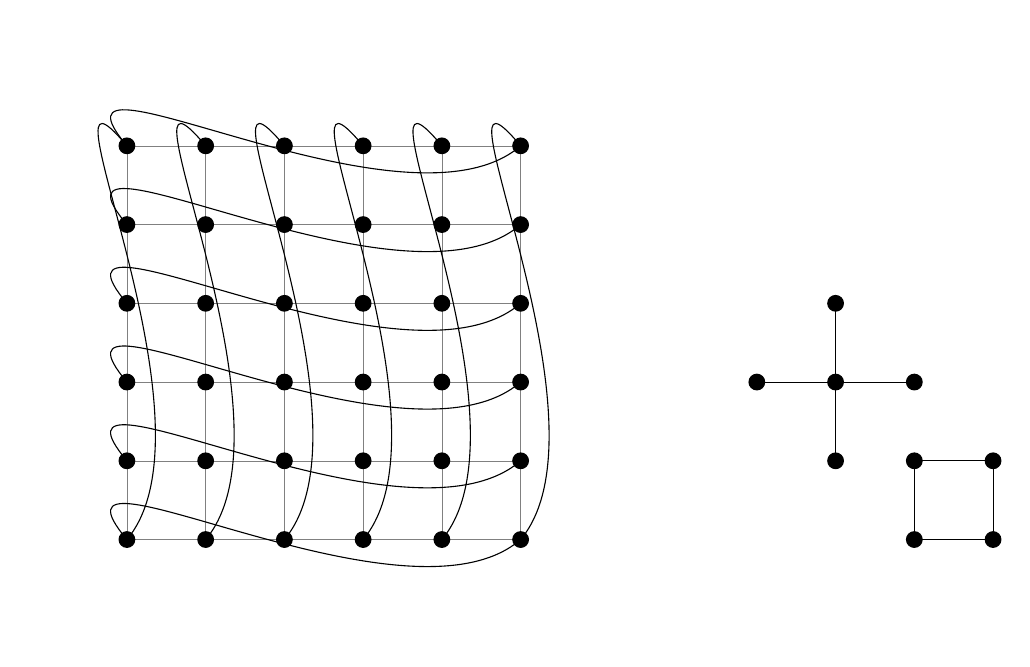
\begin{tikzpicture}
  \draw[step=1cm,gray,very thin] (0,0) grid (5,5);
  \foreach \x in {0,1,2,3,4,5}
  \foreach \y in {0,1,2,3,4,5}
  {
  \node[draw,circle,inner sep=2pt,fill] at (\x,\y) {};
}
\draw[ -> ]  (0,0) to [out=50, in=130] (0,5);
\draw[ -> ]  (1,0) to [out=50, in=130] (1,5);
\draw[ -> ]  (2,0) to [out=50, in=130] (2,5);
\draw[ -> ]  (3,0) to [out=50, in=130] (3,5);
\draw[ -> ]  (4,0) to [out=50, in=130] (4,5);
\draw[ -> ]  (5,0) to [out=50, in=130] (5,5);
\draw[ -> ]  (0,5) to [out=130, in=220] (5,5);
\draw[ -> ]  (0,4) to [out=130, in=220] (5,4);
\draw[ -> ]  (0,3) to [out=130, in=220] (5,3);
\draw[ -> ]  (0,2) to [out=130, in=220] (5,2);
\draw[ -> ]  (0,1) to [out=130, in=220] (5,1);
\draw[ -> ]  (0,0) to [out=130, in=220] (5,0);

\node[draw,circle,inner sep=2pt,fill] at (9,2) {};
\node[draw,circle,inner sep=2pt,fill] at (10,2) {};
\node[draw,circle,inner sep=2pt,fill] at (8,2) {};
\node[draw,circle,inner sep=2pt,fill] at (9,1) {};
\node[draw,circle,inner sep=2pt,fill] at (9,3) {};
\draw[ -> ]  (9,2) to (10,2);
\draw[ -> ]  (9,2) to (8,2);
\draw[ -> ]  (9,2) to (9,1);
\draw[ -> ]  (9,2) to (9,3);
%\draw[ -> ]  (9,2) to (5,0);

\node[draw,circle,inner sep=2pt,fill] at (10,1) {};
\node[draw,circle,inner sep=2pt,fill] at (11,1) {};
\node[draw,circle,inner sep=2pt,fill] at (10,0) {};
\node[draw,circle,inner sep=2pt,fill] at (11,0) {};
\draw[ -> ]  (10,1) to (11,1);
\draw[ -> ]  (10,1) to (10,0);
\draw[ -> ]  (10,0) to (11,0);
\draw[ -> ]  (11,1) to (11,0);
\end{tikzpicture}
\caption{On the left is the Toric Graph. On the right are cross and face checks.}
\label{fig:Toric}
\end{figure}
\end{center}
For example consider some vertex $v$ on the Torus, and let $\ket{\psi} = \sum_{x}{ \ket{\cdots x_{e_0}x_{e_1}x_{e_2}x_{e_3}  \cdots}}$ when $e_{0},e_{1},e_{2},e_{3}$ are the edges compose the local view of $v$. Then in any ket can be in the support of $\ket{\psi}$ only if the parity of $e_{0},e_{1},e_{2},e_{3}$ is even.
%\subsection{Note on the Toric in the presence of noise.} 

\begin{claim}
  The $l \times l$  Toric code is a CSS code, with dimension $2$ and distance $\Theta\left( l \right)$.   
\end{claim}
\begin{proof}
  Consider a pair of cross and a face checks. If they are not intersect (share edges) then, obviously, they commute. So suppose they share an edge. Now there are a finite number of cases ($4$) in which a cross check can intersect a face, and for all of them we have they must to intersect in an exactly two edges. Therefore the crosses checks commute with all the faces checks. 

  Now, denote by $C_{X}$ and $C_{Z}$ the linear codes defined by the crosses and faces checks. Observes that $C_{X}$ contain all the subgraph of the tours which have only evens degree, namely all the loops. The following claim will be used to show that all the low weight loops (squeezable loops) are in $C_{Z}^{\perp}$. 
  \begin{claim} \label{claim:square}
    Let $c$ be an assignment of ones on a unite square, namely a closed loop at length $4$, then $c \in C_{Z}^{\perp}$.  
  \end{claim}
  \begin{proof}
    Denote by $c^{\prime}$ a codeword of $C_{Z}$, therefore the parity sum induced by $c^{\prime}$ on any square equals zero, Particularly the induced parity on the square supporting $c$ is zero. But that parity is exactly $c\cdot c^{\prime}$. As it true for any $c^{\prime} \in C_{Z}$ we obtain that $c \in C_{Z}^{\perp}$.  
  \end{proof}
  \begin{claim}[Veblen's theorem] \label{claim:velen}
    The set of even subgraph is a linear space spanned by simple cycles (vertices degree equals exactly 2).
  \end{claim}
  \begin{proof}
    Let $P \subset E$ be an even subgraph then it must to have a simple cycle denote it by $P^{\prime}$, now notice that $P/P^\prime$ is also an even subgraph. To see that consider a vertex $v$, As $P^{\prime}$ is simple cycle, substituting $P^{\prime}$ is either not effect the degree of $v$ in $P/P^{\prime}$ or it decrees $v$ degree by exactly $2$ so $d_{P/P^{\prime}}\left( v \right) = d_{P}\left( v \right) - 2$. In both cases $d_{P/P^{\prime}}\left( v \right)$ is even.
    By repeating recursively until $P/P^{\prime} = \{ \emptyset \}$ we get a decomposition of $P$ into a sum of simple cycles.   
  \end{proof}

  \begin{claim}
    \label{claim:inter}
%    Associate with any vertices of the Tours a coordinates in $\mathbb{Z}_{l} \times \mathbb{Z}_{l}$. Consider a simple cycle $P$ subset of the Torus. Denote $P$ by the vertices compose it $v_{0}v_{1}..v_{k}$ arranged by order. Consider a  vertex $v_{i} \in P$ such that $\{v_{i-1}, v_{i}\}$, $\{v_{i}, v_{i+1}\}$ are at the same direaction and denote $v = \left( x,y \right) \in $$ \mathbb{Z}_{l} \times \mathbb{Z}_{l}$. Then there exist vertex $u \in P$, $ u \neq v_{i-1}v_{i+1}$ that share one of the cordinates of $v$. Put it differnetly there exsit $z$ such either  $u = \left( z,y \right)$ or $u = \left( x,z \right)$. 
Associate with any vertex of the Torus a coordinate in $\mathbb{Z}_{l} \times \mathbb{Z}_{l}$. Consider a simple cycle $P$ subset of the Torus. Denote $P$ by the vertices composing it $v_{0}v_{1}..v_{k}$ arranged in order. Consider a vertex $v_{i} \in P$ such that $\{v_{i-1}, v_{i}\}$, $\{v_{i}, v_{i+1}\}$ are in the same direction and denote $v = \left( x,y \right) \in $$ \mathbb{Z}_{l} \times \mathbb{Z}_{l}$. Then there exists a vertex $u \in P$, $ u \neq v_{i-1}v_{i+1}$ that shares one of the coordinates of $v$. Put differently, there exists $z$ such that either  $u = \left( z,y \right)$ or $u = \left( x,z \right)$.
  \end{claim}

  \begin{proof} 
Assume without loss of generality that $v_{i-1} = \left( x, y -1 \right)$ and $v_{i+1} =\left( x,y+1 \right)$. Now denote by $f$ the projection on the second coordinate, $f(a,b)= b$. and observe that for any $j$ the distance $f\left( v_{j+1}\right) - \left( v_{j}  \right)$ satisfies:
    \begin{equation*}
      \begin{split}
      f\left( v_{j+1}\right) - f \left( v_{j}  \right) = 
        \begin{cases}
          \pm \left( l - 1 \right)  & v_{j} = \left( \cdot, l -1 \right), v_{j+1} = \left( \cdot, 0  \right)  \\
          \in \{ \pm 1 , 0\} & \text{else}
        \end{cases}
      \end{split}
    \end{equation*}
    So if there is no $u \neq v_{i}$ such that $f(u) = f(v_{i}) = f(v_{i-1})+1$ then there must to be an edge $\{v_{j},v_{j+1}\}$, $v_{j} = \left( \cdot, l -1 \right)$, $ v_{j+1} = \left( \cdot, 0  \right)$ such $P$ pass trough it. So  
    \begin{equation*}
      \begin{split}
        f\left( v_{i-1} \right) & \le f\left( v+1 \right) +  |f\left( v+2 \right) -  f\left( v+1 \right)| + .. + -\left( l - 1 \right) \\ 
        & \le f(v+1) - |P| - \left(l-1\right)  
      \end{split}
    \end{equation*}
    But $|P| \le l$. 
  \end{proof}
  \begin{figure}[h]
 \begin{tikzpicture}
    \draw [thick, decorate, decoration={random steps,segment length=3pt,amplitude=1pt}]
 (1,0) to[out=90,in=90] (5,0);
    \draw [thick, decorate, decoration={random steps,segment length=3pt,amplitude=1pt}]
 (5,0) to[out=270,in=270] (1,-0.3);
 \filldraw[black] (1,0) circle (2pt) node[anchor=west]{$v_{i+1}$};
 \filldraw[black] (1,-0.3) circle (2pt) node[anchor=west]{$v_{i}$};
 \filldraw[black] (5,0) circle (2pt) node[anchor=west]{$u$};
\draw[draw=gray] (0,-3) rectangle ++(7,7);

\draw [thick, decorate, decoration={random steps,segment length=3pt,amplitude=1pt}]
 (9,0) to[out=90,in=270] (11,4);
    \draw [thick, decorate, decoration={random steps,segment length=3pt,amplitude=1pt}]
 (11,-3) to[out=90,in=270] (9,-0.3);
 \filldraw[black] (9,0) circle (2pt) node[anchor=west]{$v_{i+1}$};
 \filldraw[black] (9,-0.3) circle (2pt) node[anchor=west]{$v_{i}$};
 %\filldraw[black] (13,0) circle (2pt) node[anchor=west]{$u$};
\draw[draw=gray] (8,-3) rectangle ++(7,7);


    %\draw [thick, decorate, decoration={random steps,segment length=10pt,amplitude=2pt}]
 %(0,0) to[out=0,in=0] (0,4);
  \end{tikzpicture}
\end{figure}

  \begin{definition}
    Horizontal and Vertical diameters. Let $P$ be defined again as exactly as in \cref{claim:inter}. We will say that the \textit{horizontal diameter} of $P$ is: 
    \begin{equation*}
      \begin{split}
        \max_{v,u\in P} \min{ \left\{  | v_{x} -u_{x}|, |v_{x} + l + u_{x}| \right\} }  
      \end{split}
    \end{equation*}
    Similarly, we define the vertical diametr to be: 
    \begin{equation*}
      \begin{split}
        \max_{v,u\in P} \min{ \left\{  | v_{y} -u_{y}|, |v_{y} + l + u_{y}| \right\} }  
      \end{split}
    \end{equation*}
  \end{definition}

  \begin{claim} \label{claim:reduce}
If $P$ is a non empty simple cycle with vertical and horizontal diameters $d_{1}, d_{2}$, then it can either be a square or can be decomposed into two simple cycles $P_{1},P_{2}$ with either the vertical diameter of both of them being strictly less than $d_{1}$ and their horizontal diameters being at most $d_{2}$, or the horizontal diameter of both of them being strictly less than $d_{2}$ and their vertical diameters being at most $d_{1}$.
  \end{claim}

  \begin{proof} 
%    Assuming $P$ is not a square, it must have either a vertical or horizontal diameter greater than $1$. Let us assume, without loss of generality, that the vertical diameter is greater than $1$. Denote by $v_{0}v_{1}..v_{k}$ the vertices compose $P$, and assume that $v_{i},v_{j}$ are the vertices at maximal distace. Now Pick the first vertex $v_{i^\prime}$ form left to $v_{i}$ such that $v_{i^\prime , y} \neq v_{i,y}$. By \cref{claim:inter} there is at least one vertex $v_{l}$ in $P$ such that $v_{i,y} = v_{l,y}$ takes the one who closet in horizontal distance to $v_{i}$. Now denote by $P^{\uparrow}$ the path $v_{i},v_{i+1}..v_{l-1},v_{l}$ and by $P^{\downarrow}$ the path $v_{l},v_{l+1}..v_{i-1},v_{i}$. Denote by $L$ the stright line $v_{i},\left( v_{i,x}+1, v_{i,y} \right), \left( v_{i,x}+2, v_{i,y} \right), .. v_{l}$. 
%    Assume that both $P^{\uparrow}\cup L$,$P^{\downarrow}\cup L$ are simple cycles, Clearly the vertical diameter is lower by exectly $1$ than the vertical diameter of $P$, also the horizontal distance between any point on $L$ to other point on $P$ is lower than the horizontal distance of between the end of $L$ (namely $\{v_{i},v_{l}\}$), to the same point. Therfore In that case we have the claim.   
%    So it's left to show that $P^{\uparrow}\cup L$,$P^{\downarrow}\cup L$ must to be a simple cycles. Suppose that $P^{\uparrow}\cup L$ is not a simple cycle. So the path $v_{i},v_{i+1}..v_{l-1},v_{l}.. \left( v_{i,x}+2, v_{i,y} \right), \left( v_{i,x}+1, v_{i,y} \right)v_{i}$  must to contain an inner loop. Obivesly the loop can't be supported on $P^{\uparrow}$ alone, because $P^{\uparrow} \subset P$ so the inner loop would has to be contained also in $P$ in controdiction for $P$ be a simple cycle. Thefore, the inner loop is also supported on $L$, So it follows that there is an vertex in $L$ a vertex with degree $>2$ in $P^{\uparrow}\cup L$, namely a vetex $u \neq v_{i},v_{l}$ such that $u_{y} = v_{i,y}$, and also $u \in P$. But by the construction of $L$, $|u_{x} - v_{i,x}| < |v_{l,x} - v_{i,x}|$ in contradiction to the fact that $v_{l}$ chosen to miniazie an horizontal distance.  
%
If $P$ is not a square, it must have either a vertical or horizontal diameter greater than $1$. We will assume, without loss of generality, that the vertical diameter is greater than $1$. Let $v_{0}v_{1}..v_{k}$ be the vertices that compose $P$, and let $v_{i},v_{j}$ be the vertices at maximal distance. We will pick the first vertex $v_{i^\prime}$ from the left of $v_{i}$ such that $v_{i^\prime , y} \neq v_{i,y}$. By \cref{claim:inter}, there must be at least one vertex $v_{l}$ in $P$ such that $v_{i,y} = v_{l,y}$ and is the closest in horizontal distance to $v_{i}$. We will denote by $P^{\uparrow}$ the path $v_{i},v_{i+1}..v_{l-1},v_{l}$ and by $P^{\downarrow}$ the path $v_{l},v_{l+1}..v_{i-1},v_{i}$. We will also denote by $L$ the straight line $v_{i},\left( v_{i,x}+1, v_{i,y} \right), \left( v_{i,x}+2, v_{i,y} \right), .. v_{l}$. 

Observes that the vertical diameter will be lower by exactly $1$ than the vertical diameter of $P$, and the horizontal distance between any point on $L$ to other point on $P$ will be lower than the horizontal distance of between the end of $L$ (namely $\{v_{i},v_{l}\}$), to the same point. So if $P^{\uparrow}\cup L$,$P^{\downarrow}\cup L$ are simple cycles then we get the desire. 
Suppose that $P^{\uparrow}\cup L$ is not a simple cycle. This means that the path $v_{i},v_{i+1}..v_{l-1},v_{l}.. \left( v_{i,x}+2, v_{i,y} \right), \left( v_{i,x}+1, v_{i,y} \right)v_{i}$ must contain an inner loop. This loop cannot be supported on $P^{\uparrow}$ alone, because $P^{\uparrow} \subset P$ so the inner loop would have to be contained also in $P$, which is a contradiction. Therefore, the inner loop is also supported on $L$, so it follows that there is a vertex in $L$ with degree $>2$ in $P^{\uparrow}\cup L$, namely a vetex $u \neq v_{i},v_{l}$ such that $u_{y} = v_{i,y}$, and also $u \in P$. But by the construction of $L$, $|u_{x} - v_{i,x}| < |v_{l,x} - v_{i,x}|$, which is a contradiction to the fact that $v_{l}$ was chosen to minimize the horizontal distance. Thus, we have our claim.
  \end{proof}

%  Now we are ready to proof the claim. Let $c\in C_{X}$ such that $|c| < l$. By \cref{claim:velen}, $c$ decompise into simple cycles. Any of them at weight less than $l$. By applaying $\cref{claim:reduce}$ we have that any of them can decompise into sum of unite squres. But, by \cref{claim:square}, unit squres are in $C_{Z}^{\perp}$ and therfore $c \in C^{\perp}$. 

We have now established that $c \in C_{X}$ with $|c| < l$ can be decomposed into simple cycles, each of which has a weight less than $l$. Applying \cref{claim:reduce} recursively, we can further decompose each of these cycles into a sum of unit squares. However, \cref{claim:square} states that unit squares are in $C_{Z}^{\perp}$, so $c \in C^{\perp}$.
    \begin{wrapfigure}{R}{2cm}
%\begin{tikzpicture}
%    \draw [thick, decorate, decoration={random steps,segment length=3pt,amplitude=1pt}]
% (1,0) to[out=90,in=90] (3,0);
%    \draw [thick, decorate, decoration={random steps,segment length=3pt,amplitude=1pt}]
% (3,0) to[out=270,in=270] (1,0);
% \filldraw[black] (1,0) circle (2pt) node[anchor=east]{$v$};
% \filldraw[black] (3,0) circle (2pt) node[anchor=west]{$u$};
%\draw (1,0) -- (3,0);
%  \end{tikzpicture}
\end{wrapfigure}
%If $P$ is a non empty simple cycle with vertical and horizontal diameters $d_{1}, d_{2}$, then it can either be a square or can be decomposed into two simple cycles $P_{1},P_{2}$ with either the vertical diameter of both of them being strictly less than $d_{1}$ and their horizontal diameters being at most $d_{2}$, or the horizontal diameter of both of them being strictly less than $d_{2}$ and their vertical diameters being at most $d_{1}$.
%
  %\end{proof}

%  \begin{claim}
%  Any Simple cycle can be decmopise as sum of unite squares.     
%  \end{claim}
%
%  Let $c \in C_{X}$ at weight at most $l$ and by $G = (V,E)$ the Cayley graph of the tours, we will refer to each of the two generators of $G$ as directions. We will say that a tuple of edges $\{e_{1},e_{2}\}$ is corner of $c$ if they are both non zero coordinates of $c$ and in addition they match to different directions\footnote{On planner drawing, corner is just an horizontal edge followed by vertical edge}.        
% 
\end{proof}

%The Toric code is a topological quantum error-correcting code that encodes a single qubit of information into a two-dimensional lattice of qubits. It is a stabilizer code, meaning that it uses a set of commuting operators to detect and correct errors. The code is based on the mathematical structure of a torus, and its properties make it a powerful tool for quantum computing. It is also a fault-tolerant code, meaning that it can correct errors even when some of the qubits are faulty.
%
%\begin{center}
%  \begin{tikzpicture}
%    \begin{tikzpicture}[scale=1.000000,x=1pt,y=1pt]
\filldraw[color=white] (0.000000, -7.500000) rectangle (240.000000, 217.500000);
% Drawing wires
% Line 1: a0 W
\draw[color=black] (0.000000,210.000000) -- (240.000000,210.000000);
% Line 2: b0 W
\draw[color=black] (0.000000,195.000000) -- (240.000000,195.000000);
% Line 3: c0 W
\draw[color=black] (0.000000,180.000000) -- (240.000000,180.000000);
% Line 4: d0 W
\draw[color=black] (0.000000,165.000000) -- (240.000000,165.000000);
% Line 5: e0 W
\draw[color=black] (0.000000,150.000000) -- (240.000000,150.000000);
% Line 6: a1 W
\draw[color=black] (0.000000,135.000000) -- (240.000000,135.000000);
% Line 7: b1 W
\draw[color=black] (0.000000,120.000000) -- (240.000000,120.000000);
% Line 8: c1 W
\draw[color=black] (0.000000,105.000000) -- (240.000000,105.000000);
% Line 9: d1 W
\draw[color=black] (0.000000,90.000000) -- (240.000000,90.000000);
% Line 10: e1 W
\draw[color=black] (0.000000,75.000000) -- (240.000000,75.000000);
% Line 11: a2 W
\draw[color=black] (0.000000,60.000000) -- (240.000000,60.000000);
% Line 12: b2 W
\draw[color=black] (0.000000,45.000000) -- (240.000000,45.000000);
% Line 13: c2 W
\draw[color=black] (0.000000,30.000000) -- (240.000000,30.000000);
% Line 14: d2 W
\draw[color=black] (0.000000,15.000000) -- (240.000000,15.000000);
% Line 15: e2 W
\draw[color=black] (0.000000,0.000000) -- (240.000000,0.000000);
% Done with wires; drawing gates
% Line 18: d0 C a0
\draw (9.000000,210.000000) -- (9.000000,165.000000);
\begin{scope}
\draw[fill=white] (9.000000, 165.000000) circle(3.000000pt);
\clip (9.000000, 165.000000) circle(3.000000pt);
\draw (6.000000, 165.000000) -- (12.000000, 165.000000);
\draw (9.000000, 162.000000) -- (9.000000, 168.000000);
\end{scope}
\filldraw (9.000000, 210.000000) circle(1.500000pt);
% Line 30: d1 C a1
\draw (9.000000,135.000000) -- (9.000000,90.000000);
\begin{scope}
\draw[fill=white] (9.000000, 90.000000) circle(3.000000pt);
\clip (9.000000, 90.000000) circle(3.000000pt);
\draw (6.000000, 90.000000) -- (12.000000, 90.000000);
\draw (9.000000, 87.000000) -- (9.000000, 93.000000);
\end{scope}
\filldraw (9.000000, 135.000000) circle(1.500000pt);
% Line 42: d2 C a2
\draw (9.000000,60.000000) -- (9.000000,15.000000);
\begin{scope}
\draw[fill=white] (9.000000, 15.000000) circle(3.000000pt);
\clip (9.000000, 15.000000) circle(3.000000pt);
\draw (6.000000, 15.000000) -- (12.000000, 15.000000);
\draw (9.000000, 12.000000) -- (9.000000, 18.000000);
\end{scope}
\filldraw (9.000000, 60.000000) circle(1.500000pt);
% Line 19: d0 C b0
\draw (27.000000,195.000000) -- (27.000000,165.000000);
\begin{scope}
\draw[fill=white] (27.000000, 165.000000) circle(3.000000pt);
\clip (27.000000, 165.000000) circle(3.000000pt);
\draw (24.000000, 165.000000) -- (30.000000, 165.000000);
\draw (27.000000, 162.000000) -- (27.000000, 168.000000);
\end{scope}
\filldraw (27.000000, 195.000000) circle(1.500000pt);
% Line 31: d1 C b1
\draw (27.000000,120.000000) -- (27.000000,90.000000);
\begin{scope}
\draw[fill=white] (27.000000, 90.000000) circle(3.000000pt);
\clip (27.000000, 90.000000) circle(3.000000pt);
\draw (24.000000, 90.000000) -- (30.000000, 90.000000);
\draw (27.000000, 87.000000) -- (27.000000, 93.000000);
\end{scope}
\filldraw (27.000000, 120.000000) circle(1.500000pt);
% Line 43: d2 C b2
\draw (27.000000,45.000000) -- (27.000000,15.000000);
\begin{scope}
\draw[fill=white] (27.000000, 15.000000) circle(3.000000pt);
\clip (27.000000, 15.000000) circle(3.000000pt);
\draw (24.000000, 15.000000) -- (30.000000, 15.000000);
\draw (27.000000, 12.000000) -- (27.000000, 18.000000);
\end{scope}
\filldraw (27.000000, 45.000000) circle(1.500000pt);
% Line 20: e0 C b0
\draw (45.000000,195.000000) -- (45.000000,150.000000);
\begin{scope}
\draw[fill=white] (45.000000, 150.000000) circle(3.000000pt);
\clip (45.000000, 150.000000) circle(3.000000pt);
\draw (42.000000, 150.000000) -- (48.000000, 150.000000);
\draw (45.000000, 147.000000) -- (45.000000, 153.000000);
\end{scope}
\filldraw (45.000000, 195.000000) circle(1.500000pt);
% Line 32: e1 C b1
\draw (45.000000,120.000000) -- (45.000000,75.000000);
\begin{scope}
\draw[fill=white] (45.000000, 75.000000) circle(3.000000pt);
\clip (45.000000, 75.000000) circle(3.000000pt);
\draw (42.000000, 75.000000) -- (48.000000, 75.000000);
\draw (45.000000, 72.000000) -- (45.000000, 78.000000);
\end{scope}
\filldraw (45.000000, 120.000000) circle(1.500000pt);
% Line 44: e2 C b2
\draw (45.000000,45.000000) -- (45.000000,0.000000);
\begin{scope}
\draw[fill=white] (45.000000, 0.000000) circle(3.000000pt);
\clip (45.000000, 0.000000) circle(3.000000pt);
\draw (42.000000, 0.000000) -- (48.000000, 0.000000);
\draw (45.000000, -3.000000) -- (45.000000, 3.000000);
\end{scope}
\filldraw (45.000000, 45.000000) circle(1.500000pt);
% Line 21: e0 C c0
\draw (63.000000,180.000000) -- (63.000000,150.000000);
\begin{scope}
\draw[fill=white] (63.000000, 150.000000) circle(3.000000pt);
\clip (63.000000, 150.000000) circle(3.000000pt);
\draw (60.000000, 150.000000) -- (66.000000, 150.000000);
\draw (63.000000, 147.000000) -- (63.000000, 153.000000);
\end{scope}
\filldraw (63.000000, 180.000000) circle(1.500000pt);
% Line 33: e1 C c1
\draw (63.000000,105.000000) -- (63.000000,75.000000);
\begin{scope}
\draw[fill=white] (63.000000, 75.000000) circle(3.000000pt);
\clip (63.000000, 75.000000) circle(3.000000pt);
\draw (60.000000, 75.000000) -- (66.000000, 75.000000);
\draw (63.000000, 72.000000) -- (63.000000, 78.000000);
\end{scope}
\filldraw (63.000000, 105.000000) circle(1.500000pt);
% Line 45: e2 C c2
\draw (63.000000,30.000000) -- (63.000000,0.000000);
\begin{scope}
\draw[fill=white] (63.000000, 0.000000) circle(3.000000pt);
\clip (63.000000, 0.000000) circle(3.000000pt);
\draw (60.000000, 0.000000) -- (66.000000, 0.000000);
\draw (63.000000, -3.000000) -- (63.000000, 3.000000);
\end{scope}
\filldraw (63.000000, 30.000000) circle(1.500000pt);
% Line 22: e0 G $X$
\begin{scope}
\draw[fill=white] (84.000000, 150.000000) +(-45.000000:8.485281pt and 8.485281pt) -- +(45.000000:8.485281pt and 8.485281pt) -- +(135.000000:8.485281pt and 8.485281pt) -- +(225.000000:8.485281pt and 8.485281pt) -- cycle;
\clip (84.000000, 150.000000) +(-45.000000:8.485281pt and 8.485281pt) -- +(45.000000:8.485281pt and 8.485281pt) -- +(135.000000:8.485281pt and 8.485281pt) -- +(225.000000:8.485281pt and 8.485281pt) -- cycle;
\draw (84.000000, 150.000000) node {$X$};
\end{scope}
% Line 34: d1 e1 +b1
\draw (84.000000,120.000000) -- (84.000000,75.000000);
\filldraw (84.000000, 90.000000) circle(1.500000pt);
\filldraw (84.000000, 75.000000) circle(1.500000pt);
\begin{scope}
\draw[fill=white] (84.000000, 120.000000) circle(3.000000pt);
\clip (84.000000, 120.000000) circle(3.000000pt);
\draw (81.000000, 120.000000) -- (87.000000, 120.000000);
\draw (84.000000, 117.000000) -- (84.000000, 123.000000);
\end{scope}
% Line 46: d2 e2 +b2
\draw (84.000000,45.000000) -- (84.000000,0.000000);
\filldraw (84.000000, 15.000000) circle(1.500000pt);
\filldraw (84.000000, 0.000000) circle(1.500000pt);
\begin{scope}
\draw[fill=white] (84.000000, 45.000000) circle(3.000000pt);
\clip (84.000000, 45.000000) circle(3.000000pt);
\draw (81.000000, 45.000000) -- (87.000000, 45.000000);
\draw (84.000000, 42.000000) -- (84.000000, 48.000000);
\end{scope}
% Line 23: d0 e0 +c0
\draw (108.000000,180.000000) -- (108.000000,150.000000);
\filldraw (108.000000, 165.000000) circle(1.500000pt);
\filldraw (108.000000, 150.000000) circle(1.500000pt);
\begin{scope}
\draw[fill=white] (108.000000, 180.000000) circle(3.000000pt);
\clip (108.000000, 180.000000) circle(3.000000pt);
\draw (105.000000, 180.000000) -- (111.000000, 180.000000);
\draw (108.000000, 177.000000) -- (108.000000, 183.000000);
\end{scope}
% Line 35: d1 G $X$
\begin{scope}
\draw[fill=white] (108.000000, 90.000000) +(-45.000000:8.485281pt and 8.485281pt) -- +(45.000000:8.485281pt and 8.485281pt) -- +(135.000000:8.485281pt and 8.485281pt) -- +(225.000000:8.485281pt and 8.485281pt) -- cycle;
\clip (108.000000, 90.000000) +(-45.000000:8.485281pt and 8.485281pt) -- +(45.000000:8.485281pt and 8.485281pt) -- +(135.000000:8.485281pt and 8.485281pt) -- +(225.000000:8.485281pt and 8.485281pt) -- cycle;
\draw (108.000000, 90.000000) node {$X$};
\end{scope}
% Line 47: d2 G $X$
\begin{scope}
\draw[fill=white] (108.000000, 15.000000) +(-45.000000:8.485281pt and 8.485281pt) -- +(45.000000:8.485281pt and 8.485281pt) -- +(135.000000:8.485281pt and 8.485281pt) -- +(225.000000:8.485281pt and 8.485281pt) -- cycle;
\clip (108.000000, 15.000000) +(-45.000000:8.485281pt and 8.485281pt) -- +(45.000000:8.485281pt and 8.485281pt) -- +(135.000000:8.485281pt and 8.485281pt) -- +(225.000000:8.485281pt and 8.485281pt) -- cycle;
\draw (108.000000, 15.000000) node {$X$};
\end{scope}
% Line 58: b1 G $H$
\begin{scope}
\draw[fill=white] (108.000000, 120.000000) +(-45.000000:8.485281pt and 8.485281pt) -- +(45.000000:8.485281pt and 8.485281pt) -- +(135.000000:8.485281pt and 8.485281pt) -- +(225.000000:8.485281pt and 8.485281pt) -- cycle;
\clip (108.000000, 120.000000) +(-45.000000:8.485281pt and 8.485281pt) -- +(45.000000:8.485281pt and 8.485281pt) -- +(135.000000:8.485281pt and 8.485281pt) -- +(225.000000:8.485281pt and 8.485281pt) -- cycle;
\draw (108.000000, 120.000000) node {$H$};
\end{scope}
% Line 61: b2 G $H$
\begin{scope}
\draw[fill=white] (108.000000, 45.000000) +(-45.000000:8.485281pt and 8.485281pt) -- +(45.000000:8.485281pt and 8.485281pt) -- +(135.000000:8.485281pt and 8.485281pt) -- +(225.000000:8.485281pt and 8.485281pt) -- cycle;
\clip (108.000000, 45.000000) +(-45.000000:8.485281pt and 8.485281pt) -- +(45.000000:8.485281pt and 8.485281pt) -- +(135.000000:8.485281pt and 8.485281pt) -- +(225.000000:8.485281pt and 8.485281pt) -- cycle;
\draw (108.000000, 45.000000) node {$H$};
\end{scope}
% Line 24: e0 G $X$
\begin{scope}
\draw[fill=white] (132.000000, 150.000000) +(-45.000000:8.485281pt and 8.485281pt) -- +(45.000000:8.485281pt and 8.485281pt) -- +(135.000000:8.485281pt and 8.485281pt) -- +(225.000000:8.485281pt and 8.485281pt) -- cycle;
\clip (132.000000, 150.000000) +(-45.000000:8.485281pt and 8.485281pt) -- +(45.000000:8.485281pt and 8.485281pt) -- +(135.000000:8.485281pt and 8.485281pt) -- +(225.000000:8.485281pt and 8.485281pt) -- cycle;
\draw (132.000000, 150.000000) node {$X$};
\end{scope}
% Line 36: d1 e1 +a1
\draw (132.000000,135.000000) -- (132.000000,75.000000);
\filldraw (132.000000, 90.000000) circle(1.500000pt);
\filldraw (132.000000, 75.000000) circle(1.500000pt);
\begin{scope}
\draw[fill=white] (132.000000, 135.000000) circle(3.000000pt);
\clip (132.000000, 135.000000) circle(3.000000pt);
\draw (129.000000, 135.000000) -- (135.000000, 135.000000);
\draw (132.000000, 132.000000) -- (132.000000, 138.000000);
\end{scope}
% Line 48: d2 e2 +a2
\draw (132.000000,60.000000) -- (132.000000,0.000000);
\filldraw (132.000000, 15.000000) circle(1.500000pt);
\filldraw (132.000000, 0.000000) circle(1.500000pt);
\begin{scope}
\draw[fill=white] (132.000000, 60.000000) circle(3.000000pt);
\clip (132.000000, 60.000000) circle(3.000000pt);
\draw (129.000000, 60.000000) -- (135.000000, 60.000000);
\draw (132.000000, 57.000000) -- (132.000000, 63.000000);
\end{scope}
% Line 56: c0 G $H$
\begin{scope}
\draw[fill=white] (132.000000, 180.000000) +(-45.000000:8.485281pt and 8.485281pt) -- +(45.000000:8.485281pt and 8.485281pt) -- +(135.000000:8.485281pt and 8.485281pt) -- +(225.000000:8.485281pt and 8.485281pt) -- cycle;
\clip (132.000000, 180.000000) +(-45.000000:8.485281pt and 8.485281pt) -- +(45.000000:8.485281pt and 8.485281pt) -- +(135.000000:8.485281pt and 8.485281pt) -- +(225.000000:8.485281pt and 8.485281pt) -- cycle;
\draw (132.000000, 180.000000) node {$H$};
\end{scope}
% Line 25: d0 e0 +b0
\draw (156.000000,195.000000) -- (156.000000,150.000000);
\filldraw (156.000000, 165.000000) circle(1.500000pt);
\filldraw (156.000000, 150.000000) circle(1.500000pt);
\begin{scope}
\draw[fill=white] (156.000000, 195.000000) circle(3.000000pt);
\clip (156.000000, 195.000000) circle(3.000000pt);
\draw (153.000000, 195.000000) -- (159.000000, 195.000000);
\draw (156.000000, 192.000000) -- (156.000000, 198.000000);
\end{scope}
% Line 37: d1 G $X$
\begin{scope}
\draw[fill=white] (156.000000, 90.000000) +(-45.000000:8.485281pt and 8.485281pt) -- +(45.000000:8.485281pt and 8.485281pt) -- +(135.000000:8.485281pt and 8.485281pt) -- +(225.000000:8.485281pt and 8.485281pt) -- cycle;
\clip (156.000000, 90.000000) +(-45.000000:8.485281pt and 8.485281pt) -- +(45.000000:8.485281pt and 8.485281pt) -- +(135.000000:8.485281pt and 8.485281pt) -- +(225.000000:8.485281pt and 8.485281pt) -- cycle;
\draw (156.000000, 90.000000) node {$X$};
\end{scope}
% Line 38: e1 G $X$
\begin{scope}
\draw[fill=white] (156.000000, 75.000000) +(-45.000000:8.485281pt and 8.485281pt) -- +(45.000000:8.485281pt and 8.485281pt) -- +(135.000000:8.485281pt and 8.485281pt) -- +(225.000000:8.485281pt and 8.485281pt) -- cycle;
\clip (156.000000, 75.000000) +(-45.000000:8.485281pt and 8.485281pt) -- +(45.000000:8.485281pt and 8.485281pt) -- +(135.000000:8.485281pt and 8.485281pt) -- +(225.000000:8.485281pt and 8.485281pt) -- cycle;
\draw (156.000000, 75.000000) node {$X$};
\end{scope}
% Line 49: d2 G $X$
\begin{scope}
\draw[fill=white] (156.000000, 15.000000) +(-45.000000:8.485281pt and 8.485281pt) -- +(45.000000:8.485281pt and 8.485281pt) -- +(135.000000:8.485281pt and 8.485281pt) -- +(225.000000:8.485281pt and 8.485281pt) -- cycle;
\clip (156.000000, 15.000000) +(-45.000000:8.485281pt and 8.485281pt) -- +(45.000000:8.485281pt and 8.485281pt) -- +(135.000000:8.485281pt and 8.485281pt) -- +(225.000000:8.485281pt and 8.485281pt) -- cycle;
\draw (156.000000, 15.000000) node {$X$};
\end{scope}
% Line 50: e2 G $X$
\begin{scope}
\draw[fill=white] (156.000000, -0.000000) +(-45.000000:8.485281pt and 8.485281pt) -- +(45.000000:8.485281pt and 8.485281pt) -- +(135.000000:8.485281pt and 8.485281pt) -- +(225.000000:8.485281pt and 8.485281pt) -- cycle;
\clip (156.000000, -0.000000) +(-45.000000:8.485281pt and 8.485281pt) -- +(45.000000:8.485281pt and 8.485281pt) -- +(135.000000:8.485281pt and 8.485281pt) -- +(225.000000:8.485281pt and 8.485281pt) -- cycle;
\draw (156.000000, -0.000000) node {$X$};
\end{scope}
% Line 57: a1 G $H$
\begin{scope}
\draw[fill=white] (156.000000, 135.000000) +(-45.000000:8.485281pt and 8.485281pt) -- +(45.000000:8.485281pt and 8.485281pt) -- +(135.000000:8.485281pt and 8.485281pt) -- +(225.000000:8.485281pt and 8.485281pt) -- cycle;
\clip (156.000000, 135.000000) +(-45.000000:8.485281pt and 8.485281pt) -- +(45.000000:8.485281pt and 8.485281pt) -- +(135.000000:8.485281pt and 8.485281pt) -- +(225.000000:8.485281pt and 8.485281pt) -- cycle;
\draw (156.000000, 135.000000) node {$H$};
\end{scope}
% Line 60: a2 G $H$
\begin{scope}
\draw[fill=white] (156.000000, 60.000000) +(-45.000000:8.485281pt and 8.485281pt) -- +(45.000000:8.485281pt and 8.485281pt) -- +(135.000000:8.485281pt and 8.485281pt) -- +(225.000000:8.485281pt and 8.485281pt) -- cycle;
\clip (156.000000, 60.000000) +(-45.000000:8.485281pt and 8.485281pt) -- +(45.000000:8.485281pt and 8.485281pt) -- +(135.000000:8.485281pt and 8.485281pt) -- +(225.000000:8.485281pt and 8.485281pt) -- cycle;
\draw (156.000000, 60.000000) node {$H$};
\end{scope}
% Line 26: d0 G $X$
\begin{scope}
\draw[fill=white] (180.000000, 165.000000) +(-45.000000:8.485281pt and 8.485281pt) -- +(45.000000:8.485281pt and 8.485281pt) -- +(135.000000:8.485281pt and 8.485281pt) -- +(225.000000:8.485281pt and 8.485281pt) -- cycle;
\clip (180.000000, 165.000000) +(-45.000000:8.485281pt and 8.485281pt) -- +(45.000000:8.485281pt and 8.485281pt) -- +(135.000000:8.485281pt and 8.485281pt) -- +(225.000000:8.485281pt and 8.485281pt) -- cycle;
\draw (180.000000, 165.000000) node {$X$};
\end{scope}
% Line 39: d1 e1 +c1
\draw (180.000000,105.000000) -- (180.000000,75.000000);
\filldraw (180.000000, 90.000000) circle(1.500000pt);
\filldraw (180.000000, 75.000000) circle(1.500000pt);
\begin{scope}
\draw[fill=white] (180.000000, 105.000000) circle(3.000000pt);
\clip (180.000000, 105.000000) circle(3.000000pt);
\draw (177.000000, 105.000000) -- (183.000000, 105.000000);
\draw (180.000000, 102.000000) -- (180.000000, 108.000000);
\end{scope}
% Line 51: d2 e2 +c2
\draw (180.000000,30.000000) -- (180.000000,0.000000);
\filldraw (180.000000, 15.000000) circle(1.500000pt);
\filldraw (180.000000, 0.000000) circle(1.500000pt);
\begin{scope}
\draw[fill=white] (180.000000, 30.000000) circle(3.000000pt);
\clip (180.000000, 30.000000) circle(3.000000pt);
\draw (177.000000, 30.000000) -- (183.000000, 30.000000);
\draw (180.000000, 27.000000) -- (180.000000, 33.000000);
\end{scope}
% Line 55: b0 G $H$
\begin{scope}
\draw[fill=white] (180.000000, 195.000000) +(-45.000000:8.485281pt and 8.485281pt) -- +(45.000000:8.485281pt and 8.485281pt) -- +(135.000000:8.485281pt and 8.485281pt) -- +(225.000000:8.485281pt and 8.485281pt) -- cycle;
\clip (180.000000, 195.000000) +(-45.000000:8.485281pt and 8.485281pt) -- +(45.000000:8.485281pt and 8.485281pt) -- +(135.000000:8.485281pt and 8.485281pt) -- +(225.000000:8.485281pt and 8.485281pt) -- cycle;
\draw (180.000000, 195.000000) node {$H$};
\end{scope}
% Line 27: d0 e0 +a0
\draw (204.000000,210.000000) -- (204.000000,150.000000);
\filldraw (204.000000, 165.000000) circle(1.500000pt);
\filldraw (204.000000, 150.000000) circle(1.500000pt);
\begin{scope}
\draw[fill=white] (204.000000, 210.000000) circle(3.000000pt);
\clip (204.000000, 210.000000) circle(3.000000pt);
\draw (201.000000, 210.000000) -- (207.000000, 210.000000);
\draw (204.000000, 207.000000) -- (204.000000, 213.000000);
\end{scope}
% Line 40: e1 G $X$
\begin{scope}
\draw[fill=white] (204.000000, 75.000000) +(-45.000000:8.485281pt and 8.485281pt) -- +(45.000000:8.485281pt and 8.485281pt) -- +(135.000000:8.485281pt and 8.485281pt) -- +(225.000000:8.485281pt and 8.485281pt) -- cycle;
\clip (204.000000, 75.000000) +(-45.000000:8.485281pt and 8.485281pt) -- +(45.000000:8.485281pt and 8.485281pt) -- +(135.000000:8.485281pt and 8.485281pt) -- +(225.000000:8.485281pt and 8.485281pt) -- cycle;
\draw (204.000000, 75.000000) node {$X$};
\end{scope}
% Line 52: e2 G $X$
\begin{scope}
\draw[fill=white] (204.000000, -0.000000) +(-45.000000:8.485281pt and 8.485281pt) -- +(45.000000:8.485281pt and 8.485281pt) -- +(135.000000:8.485281pt and 8.485281pt) -- +(225.000000:8.485281pt and 8.485281pt) -- cycle;
\clip (204.000000, -0.000000) +(-45.000000:8.485281pt and 8.485281pt) -- +(45.000000:8.485281pt and 8.485281pt) -- +(135.000000:8.485281pt and 8.485281pt) -- +(225.000000:8.485281pt and 8.485281pt) -- cycle;
\draw (204.000000, -0.000000) node {$X$};
\end{scope}
% Line 59: c1 G $H$
\begin{scope}
\draw[fill=white] (204.000000, 105.000000) +(-45.000000:8.485281pt and 8.485281pt) -- +(45.000000:8.485281pt and 8.485281pt) -- +(135.000000:8.485281pt and 8.485281pt) -- +(225.000000:8.485281pt and 8.485281pt) -- cycle;
\clip (204.000000, 105.000000) +(-45.000000:8.485281pt and 8.485281pt) -- +(45.000000:8.485281pt and 8.485281pt) -- +(135.000000:8.485281pt and 8.485281pt) -- +(225.000000:8.485281pt and 8.485281pt) -- cycle;
\draw (204.000000, 105.000000) node {$H$};
\end{scope}
% Line 62: c2 G $H$
\begin{scope}
\draw[fill=white] (204.000000, 30.000000) +(-45.000000:8.485281pt and 8.485281pt) -- +(45.000000:8.485281pt and 8.485281pt) -- +(135.000000:8.485281pt and 8.485281pt) -- +(225.000000:8.485281pt and 8.485281pt) -- cycle;
\clip (204.000000, 30.000000) +(-45.000000:8.485281pt and 8.485281pt) -- +(45.000000:8.485281pt and 8.485281pt) -- +(135.000000:8.485281pt and 8.485281pt) -- +(225.000000:8.485281pt and 8.485281pt) -- cycle;
\draw (204.000000, 30.000000) node {$H$};
\end{scope}
% Line 28: d0 G $X$
\begin{scope}
\draw[fill=white] (228.000000, 165.000000) +(-45.000000:8.485281pt and 8.485281pt) -- +(45.000000:8.485281pt and 8.485281pt) -- +(135.000000:8.485281pt and 8.485281pt) -- +(225.000000:8.485281pt and 8.485281pt) -- cycle;
\clip (228.000000, 165.000000) +(-45.000000:8.485281pt and 8.485281pt) -- +(45.000000:8.485281pt and 8.485281pt) -- +(135.000000:8.485281pt and 8.485281pt) -- +(225.000000:8.485281pt and 8.485281pt) -- cycle;
\draw (228.000000, 165.000000) node {$X$};
\end{scope}
% Line 54: a0 G $H$
\begin{scope}
\draw[fill=white] (228.000000, 210.000000) +(-45.000000:8.485281pt and 8.485281pt) -- +(45.000000:8.485281pt and 8.485281pt) -- +(135.000000:8.485281pt and 8.485281pt) -- +(225.000000:8.485281pt and 8.485281pt) -- cycle;
\clip (228.000000, 210.000000) +(-45.000000:8.485281pt and 8.485281pt) -- +(45.000000:8.485281pt and 8.485281pt) -- +(135.000000:8.485281pt and 8.485281pt) -- +(225.000000:8.485281pt and 8.485281pt) -- cycle;
\draw (228.000000, 210.000000) node {$H$};
\end{scope}
% Done with gates; drawing ending labels
% Done with ending labels; drawing cut lines and comments
% Line 64: a0 e0 @ 1 7
% Done with comments
\end{tikzpicture}

%  \end{tikzpicture}
%\end{center}

%\begin{algorithm}[H]
%  \caption{Shor code decoder.}
%    \label{alg:shordecoder}
%    \KwData{ $ \ket{\psi} \in \mathbb{C}_{2}^{9}$ }
%    \KwResult{ Correct a single fault. }
%    Let $D$ be a decoder for the classic repetition code over $3$ qubits. \\ 
%    Let $\ket{x_{1}x_{2}x_{3}} \leftarrow \ket{\psi}$ \\ 
%
%    $ L \leftarrow \text{Array} \{ \} $\\
%    \For { $ v \in V$} {
%      $c^{\prime}_{v} \leftarrow \arg\min {\left\{  y \in C_{0} : |y + x|_{v} |  \right\} } $\\
%      $ L_{v} \leftarrow c^{\prime}_{v}$
%    }
%    $ z \leftarrow \sum_{v \in V}{c^{\prime}_{v}} $\\
%    \eIf{ $ |z| < \tau \frac{n}{f\left( n \right)} $}{
%      \While{ $|z| > 0$ }{
%	find $v$ and $c \in C_{0}$ such that $|z + c_{v}| < |z|$\\
%	$z \leftarrow z + c_{v}$ \\
%	$ L_{v} \leftarrow  L_{v} + c_{v}$
%      }
%    }{
%      reject. 
%    }
%    \Return  $S(L) $
%
%  \end{algorithm}

%
%By quadric the dimension of the repetition code one can find those state which at least two pauli are needed to applay for flipping either the bit or the phase of the logic state. Clearly any phase flip 
 
\section{Quantum Expander Codes.}
%As similar to the classical case, the next natural question to ask is whether there are codes with positive rate. The quantum expanders were the first quantum LDPC codes to achieve a square root distance and positive rate \cite{Tillich_2014, Leverrier_2015}. The leading insight was the idea that the Toric code could be represented as a variant product of the repetition code.  For example, consider the cross restriction in figure \cref{fig:Toric}, that restriction can be obtained by gluing two vertices of two different cycle graphs. 
As similar to the classical case, the next natural question to ask is whether there are codes with positive rates. The quantum expanders were the first quantum LDPC codes to achieve a square-root distance and positive rate \cite{Tillich_2014, Leverrier_2015}. The leading insight was the idea that the Toric code could be represented as a variant product of the repetition code. For example, consider the cross restriction in Figure \cref{fig:Toric}; that restriction can be obtained by gluing two vertices of two different cycle graphs.

\begin{definition}
  For any two matrices $A,B$, with the same number of rows, denote by $\left[ A,B \right]$ the matrix obtained by attach $B$ next to $A$ from right.  Let $H_{1}, H_{2} \in \mathbb{F}_{2}^{n\times r}$ be the parity check matrices. Define the bit and the phase parity checks matrices to be:          
\begin{equation*}
  \begin{split}
    H_{X} &= \left[ H_{1} \otimes I_{r} \ \  I_{n} \otimes H^{\top}_{2} \right] \\ 
    H_{Z} &= \left[ I_{r} \otimes H_{2} \ \  H_{1}^{\top} \otimes I_{n} \right] \\ 
  \end{split}
  \label{equ:css}
\end{equation*}
The matrices are orthogonal to each other as $H_{X}H_{Z}^{\top} = H_{1}\otimes H^{\top}_{2} + H_{1}\otimes H^{\top}_{2} = 0$ and therefore the pair define a valid CSS code. We will call to that code the Hyperproduct and denote it by $Q\left( H_{1} \times H_{2} \right)$.
\end{definition}
Obliviously, if $H_{1},H_{2},H_{1}^{\top},H_{2}^{\top}$ are parity checks matrices of an LDPC codes, so are $H_{X},H_{Z}$ as their maximal row weight is at most two times larger.   
%\ref{equ:css}

% That insight raise the following perspective. The Toric code could be thought as tanner code defined on product of two cycles. If the checks in the repetition code are of the form $H_i =  x_i + x_{i+1}$  then in the Toric code the checks are $x_{i,j}+ x_{i, j+1} + x_{i+1, j} + x_{i+1,j+1}$. Namely any restriction over the edge in the Toric code  $x_{e_{0}}+ x_{e_{1}} + x_{e_{2}} + x_{e_{3}} = 0$ is obtained by taking two restrictions of the repetition code and multiple them.

\begin{sagesilent}
latex.matrix_delimiters('[', ']')
M = matrix(GF(2), [1 for _ in range(3)])
repetition = codes.LinearCode(M)
H = repetition.parity_check_matrix().stack( matrix(GF(2), [1,1,0]))
H1 = identity_matrix(3).tensor_product(H).augment( H.transpose().tensor_product(identity_matrix(3)))
Hstr = latex(H)
H1str = latex(H1)
\end{sagesilent}

\begin{example}
  The Toric code could be thought as the Hyperproduct of the repetition code with himself. The parity check matrices of the codes are given follow. The left $3 \times 3$ matrix corresponds to the repetition code while the right $18 \times  9$ corresponds to the vertices check of the Toric code.  
\end{example}

\begin{equation*}
  \begin{split}
    \sagestr{Hstr} \sagestr{H1str} 
  \end{split}
\end{equation*}


\begin{claim}
  \label{claim:kerdim}
  Let  $A,B \in \mathbb{M}_{n\times r_{1}}, \mathbb{M}_{n\times r_{2}}$ then  $\dim \ker [A ,B]$ is $ \dim \ker A + n $. 
\end{claim}

\begin{proof}
  The proof is omitted. 
\end{proof}

\begin{claim}
  Let $k_{1},k_{2}$ be the demission of the codes with the full rank  parity check matrices $H_{1},H_{2}$. Then the dimension of the Hyperproduct code is $ \ge k_{1}k_{2}$. 
\end{claim}

\begin{proof}
  %We will find the dimensions of each of the classics codes defined by $H_{X}$ and $H_{Z}$. Notice that length of the code, assuming the fullness of the ranks, is $n^{2} +  (n-k_{1}) \cdot \left( n -k_{2}\right)$. Note that for any $u,v$ such $H_{1}u = 0$ and $H_{2}^{\top}v =0$ it holds that $[u\otimes e_{i} \ e_{j}\otimes v]$ is a codeword, where $e_{i},e_{j}$ are taken from the standard basis of $[n],[n-k_{2}]$. Thus the dimension of $\ker H_{X}$ is $k_{1}n + (n-k_{1})(n-k_{2})$. 
  %By the same arguments we have that $\dim C_{Z} = k_{2}n + (n-k_{1})(n-k_{2})$. 

  We will find the dimensions of each of the classical codes defined by $\ker H_{X}$ and $ \ker H_{Z}$. Notice that the length of the $H \otimes I_{n}$ equals $n\times n = n^2$, And  assuming the fullness of the ranks, the length of $ I_{r_{1}} \otimes  H_{2}^{\top} $  is $ r_{1}\cdot r_{2}$. Thus the length of $ \ker H_{X}$ is  $n^{2} + r_{1}r_{2}$ 
  %(n-k_{1}) \cdot \left( n -k_{2}\right)$. 
  Now, recall that for any matrix $A$ it holds that $\dim \ker \left( A \otimes I_{l} \right) = l \cdot \dim \ker A$. Therefore using \cref{claim:kerdim} we obtain that the dimension of $\ker H_{X}$ is $k_{1}n + r_{1}r_{2}$ 
  %(n-k_{1})(n-k_{2})$. Using  

  By the same arguments we have that $\dim C_{Z} = k_{2}n + r_{1}r_{2}$ % (n-k_{1})(n-k_{2})$.
Thus the dimension of the quantum code is:
  \begin{equation*}
    \begin{split}
      \dim Q\left( C_{X}, C_{Z} \right) &= \dim C_{X} + \dim C_{Z} - \left(  n^{2} + (n-k_{1})(n-k_{2})  \right) \\ 
      & = \left( k_{1} + k_{2} \right)n + 2(n-k_{1})(n-k_{2}) -\left(  n^{2} +  (n-k_{1}) \cdot \left( n -k_{2}\right) \right) \\
      & =k_{1}k_{2} 
    \end{split}
  \end{equation*}
\end{proof}

\begin{remark}
  \label{remark:pun}
  Let $H_{1}^{\prime}$ be a parity check matrix obtained by puncturing columns from $H_{1}$, denote by $k^{\prime}_{1}$ the dimension of that code. Then the Hyperproduct $Q(H_{1}^{\prime}\times H_{2})$ is a CSS code with dimension $k^{\prime}_{1}k_{2}$. Moreover if the number of columns left after the puncturing is less the distance of $\ker H_{1}$ then it must to holds that $k^{\prime}_{1} = 0 \Rightarrow \dim Q(H_{1}^{\prime} \times H_{2}) = 0$. Otherwise, one can take a non trivial codeword of $\ker H^{\prime}_{1}$ and extending it to a valid codeword of $\ker H_{1}$ by set any punctured coordinate of it to zero. The yielded codeword has weight less than $d$ which is contradiction.  
\end{remark}

\begin{claim}
  \label{claim:Hdis}
  Denote by $d$ the minimal distance of $\ker H_{1}$. Any codeword $x$ of $C_{X} = \ker H_{X}$ with edge at most $d$ belongs to $C_{Z}^{\perp}$.  
\end{claim}

\begin{proof}
  Define by $H^{\prime}_{1}$ the matrix which obtained by puncturing from $H_{1}$ the columns  associated with the coordinates $e_{i}$ such that subspace corresponding to $ e_{i} \otimes I_{n} $ doesn't support $x$. Denote the by $S$ the set of the reaming coordinates.  For example if $ H_{1} \otimes I_{n} = I_{2} \otimes I_{2}$ and $x = [1,0,0,0]$ then $H^{\prime}_{1} $ is the unit matrix $[1 , 0]^\top$ obtained by puncturing the second column of $H_{1} = I_{2}$, and $S= \{ e_{1} \} $ .  


  As $|x| < d $ we have that $|S| < d$, Namely $H^{\prime}_{1}$ supported on less than $d$ coordinates and therefore $\dim Q\left( H^{\prime}_{1} \times H_{2} \right)= k^{\prime}_{1}k_{2} = 0$.  Thus, by the fact that for any CSS code $\dim C = \dim C_{X} - \dim C_{Z}^\perp$ it follows that $\dim \ker H_{X}^{\prime}  = \dim \ker H_{Z}^{\prime \perp}$ $ \Rightarrow \ker H_{X}^{\prime}  = \ker H_{Z}^{\prime \perp}$.  Denote by $x^{\prime}$ the restriction of $x$ to the columns of $H_{X}^{\prime}$ and clearly, by the definition of the construction,  $x^{\prime}$ is a codeword of $\ker H_{X}^{\prime}$. Thus $x^{\prime}$ is also codeword of $\ker H_{Z}^{\prime \perp}$ and by the same argument, $x$ is also a codeword of $\ker H_{Z}^{\prime \perp}$. 
\end{proof}

Immediately from \cref{claim:Hdis} we obtain that existences of quantum LDPC codes with positive rate and $\Theta\left( \sqrt{n} \right)$ distance by taking the Hyperproduct of two classical expender codes.   

\begin{theorem}
  There exists an infinity family of QLDPC codes with positive rate and $\Theta(\sqrt{n})$ distance.   
\end{theorem}

%\section{Quantum Codes.}
%\begin{definition}
%  A $\left[\left[ n,k,d \right]\right]$ is a quantum code over $n$ qubits, that encode a subspace at demission $k$ and any fault composed by a product of at most $d/2$ Pauli operators. 
%\end{definition}
%



%\printbibliography[heading=subbibliography]


\chapter{Good qLDPC Codes and LTC.}

The existence of good QLDPC codes and LTC were considered open problems for roughly two decades. Even though they seemed to be related only by containing the word "code" in their title, they were proven to exist by the same construction. They first appeared in \cite{Dinur} as good locally testable codes and not long after that in \cite{Pavel}, in which they also extended and derived the result to obtain the quantum code. Here, we follow the \cite{leverrier2022quantum} work, which simplifies the original proof and doesn't rely on any concept more complicated than what we already saw in the previous chapters. They also coined the term "Quantum Tanner Codes".


\section{Quantum Tanner Codes.}
Recall our insight that for a pair of LDPC codes to define a good CSS code, it must hold that neither of them is a good code, and moreover they both have a constant distance. Therefore, we understand that any codeword in $C_{X}$ that has small weight belongs to $C_{Z}^\perp$. To prove it, we are going to come up with a construction such that if $x \in C_{X}$ and $|x|$ is small then there is some small codeword $z \in C_{Z}^{\perp}$ such that $|x+z| < |x|$; by repeating this process recursively it follows that $x\in C_{Z}^{\perp}$. To formulate this theorem we will need the following definitions:
  
  \begin{definition} Let $C = \Tann$. We say that $x \in C_{\oplus}$ is \textbf{reducible} if there exists a vertex $v$ and a small codeword $c_v$, for which, adding the assignment of $c_v$ over the $v$'s edges to $x$ decreases the weight. Namely, $|x + c_{v}| < |x|$. If $x \in C_{\oplus}$ is not a reducible codeword then we say that $x$ is \textbf{irreducible} \label{ire}. \end{definition}

The next two definitions are concerned with the properties of the small code that will be set on the edges. Using them, one can characterize cases in which a local view can be reduced by subtracting a codeword from the dual code.

\begin{definition}[$w$-Robustness] 
  \label{def:wrobust}
Let $C_0$ be a code of length $\Delta$ with minimum distance $\delta_0\Delta$. $C = \duC $ will be said to be $w$-robust if for any codeword $c \in C$ of weight less than $w$, it follows that $c$ can be decomposed into a sum of $c = t + s$ such that $t \in C_A \otimes \mathbb{F}^{B}$ and $s \in \mathbb{F}^A \otimes C_B$, where $s$ and $t$ are each supported on at most $\frac{w}{\delta_0\Delta}$ rows and columns. For convenience, we will denote by $B'$ ($A'$) the rows (columns) supporting $t$ ($s$) and use the notation $t \in C_A \otimes \mathbb{F}^{B'}$.
\end{definition}

\begin{figure}[H]
  \label{fig:wrobustf}
  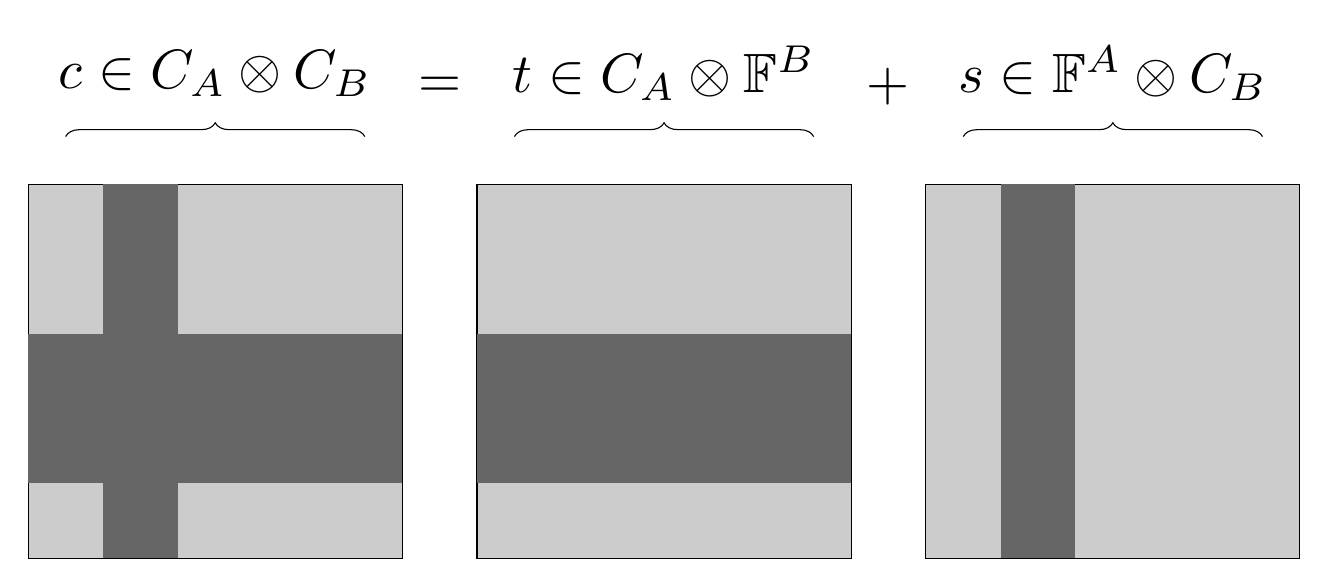
\begin{tikzpicture}[scale=0.95]

    \draw (5.5,6.3) node[scale=2]  { $=$ };
    \draw (11.5,6.3) node[scale=2]  { $+$ };

\draw [decorate,decoration={brace,amplitude=5pt,raise=4ex}] 
(0.5,5) -- (4.5,5) node[scale=2,midway,yshift=2em]{$c \in C_{A}\otimes C_{B}$};
        \filldraw [fill=white!80!black](0,0) rectangle (5,5);
       \fill [fill=gray!80!black] (1,0) rectangle (2,5);
        \fill [fill=gray!80!black] (0,1) rectangle (5,3);
\filldraw [fill=white!80!black](6,0) rectangle (11,5);
 \draw [decorate,decoration={brace,amplitude=5pt,raise=4ex}] 
 (6.5,5) -- (10.5,5) node[scale=2,midway,yshift=2em]{$t \in C_{A}\otimes \mathbb{F}^{B}$};
       \fill [fill=gray!80!black,draw opacity=0.5] (6,1) rectangle (11,3);
\filldraw [fill=white!80!black](12,0) rectangle (17,5);
  \draw [decorate,decoration={brace,amplitude=5pt,raise=4ex}] 
  (12.5,5) -- (16.5,5) node[scale=2,midway,yshift=2em]{$s \in \mathbb{F}^{A}\otimes C_{B}$};
     \fill [fill=gray!80!black,draw opacity=0.5] (13,0) rectangle (14,5);
            \end{tikzpicture}
            \caption{$w$-Robustness, Any low-weight codeword of the dual tensor code $c$ can be decomposed into a sum $t+s$, where $t$ is a collection of rows, each of which is a codeword in $C_A$, and similarly $s$ is a collection of columns, each of which is a codeword of $C_B$. }
\end{figure}



The definition we gave for $w$-Robustness is identical to the one stated by Zemor and Leverrier, but we also included the decomposition property in the definition. We refer the readers to the appendix section in \cite{leverrier2022quantum} for an existence proof by random construction. We mention that the random construction also gives the Gilbert-Varshamov bound.

\begin{definition}[$p$-Resistance to Puncturing.] Let $p,w$ be integers. We will say that the dual tensor code $C_{A} \otimes \mathbb{F} + \mathbb{F} \otimes C_{B}$ is $w$-robust with $p$-resistance to puncturing, if the code obtained by removing (puncturing) a subset of at most $p$ rows and columns is $w$-robust.   
\end{definition}

\begin{definition}[Quantum Tanner Code.]

%  Let $\Gamma$ be a group on $n$ verices. And let $A,B$ be a two generator set of $\Gamma$ such that if $a \in A$ ($B$) then also $a^{-1}\in A$ and that for any $g\in \Gamma,a \in A, b \in B$ it holds that $g \neq agb$ . Define the left right Cayley complex to be the graph $G = \left( \Gamma, E \right) $ obtain by taking the union of the two Cayley graphs generated by $A$ and $B$. So the vertices pair $u,v$ are set on square diaginal only if there are $a\in A$ and $b \in B$ such that $u = avb$. We can assume that $G$ is a bipartite graph (otherise just take $\Gamma^{\prime} = \Gamma \times \mathbb{Z}_{2}$ and define the product to be $a\left( u,\pm \right) = \left( au, \mp \right)$). 
%
%  Now divide the graph into postivie and negative vertices according their coloring $V^{-}$ and $V^{+}$. And define the positive graph to be $G^{+} = \left( V^{+}, E \right)$ and by $G^{-} = \left( V^{-}, E \right)$ the negative graph, when $E$denotes the sqaures, put it defrently their is an edge between $v$ and $u$ in $G^{+}$ if both vertices are positive and they are lay on the ends of square's diongal.
%
%  The quantum tanner code is a CSS code, such $C_{X}$ defined to be the classical tanner code $\mathcal{T}\left(G^{+}, \left(C_{A}^\perp\otimes C_{B}^{\perp}\right)^{\perp} \right)$ and $C_{Z}$ define as $\mathcal{T}\left(G^{-}, \left(C_{A}\otimes C_{B}\right)^{\perp} \right)$. Noice that in contrast to classical tanner code, in the quantum case it will be more convinent to think codewords as assiments set on the squaers and not on the edges.  
%
  Let $\Gamma$ be a group at size $n$. And let $A,B$ be a two generator set of $\Gamma$ such that if $a \in A$ ($B$) then also $a^{-1}\in A$ ($B^{-1}$) and that for any $g\in \Gamma, a \in A, b \in B$ it holds that $g \neq agb$. Define the left-right Cayley complex to be the graph $G = \left( \Gamma, E \right)$ obtained by taking the union of the two Cayley graphs generated by $A$ and $B$. So the vertices pair $u,v$ are set on a square diagonal only if there are $a\in A$ and $b \in B$ such that $u = avb$. We can assume that $G$ is a bipartite graph (otherwise just take $\Gamma^{\prime} = \Gamma \times \mathbb{Z}_{2}$ and define the product to be $a\left( u,\pm \right) = \left( au, \mp \right)$). 


Now divide the graph into positive and negative vertices according to their coloring $V^{-}$ and $V^{+}$. And define the positive graph to be $G^{+} = \left( V^{+}, E \right)$ and by $G^{-} = \left( V^{-}, E \right)$ the negative graph, where $E$ denotes the squares, put differently there is an edge between $v$ and $u$ in $G^{+}$ if both vertices are positive and they are laid on the ends of a square's diagonal.


The quantum Tanner code is a CSS code, such that $C_{X}$ is defined to be the classical Tanner code $\mathcal{T}\left(G^{+}, \left(C_{A}^\perp\otimes C_{B}^{\perp}\right)^{\perp} \right)$ and $C_{Z}$ is defined as $\mathcal{T}\left(G^{-}, \left(C_{A}\otimes C_{B}\right)^{\perp} \right)$. Note that in contrast to the classical Tanner code, in the quantum case it will be more convenient to think of codewords as assignments set on the squares and not on the edges.
\end{definition}
\begin{figure}[H]
            %\label{fig:square}
            \begin{center}
            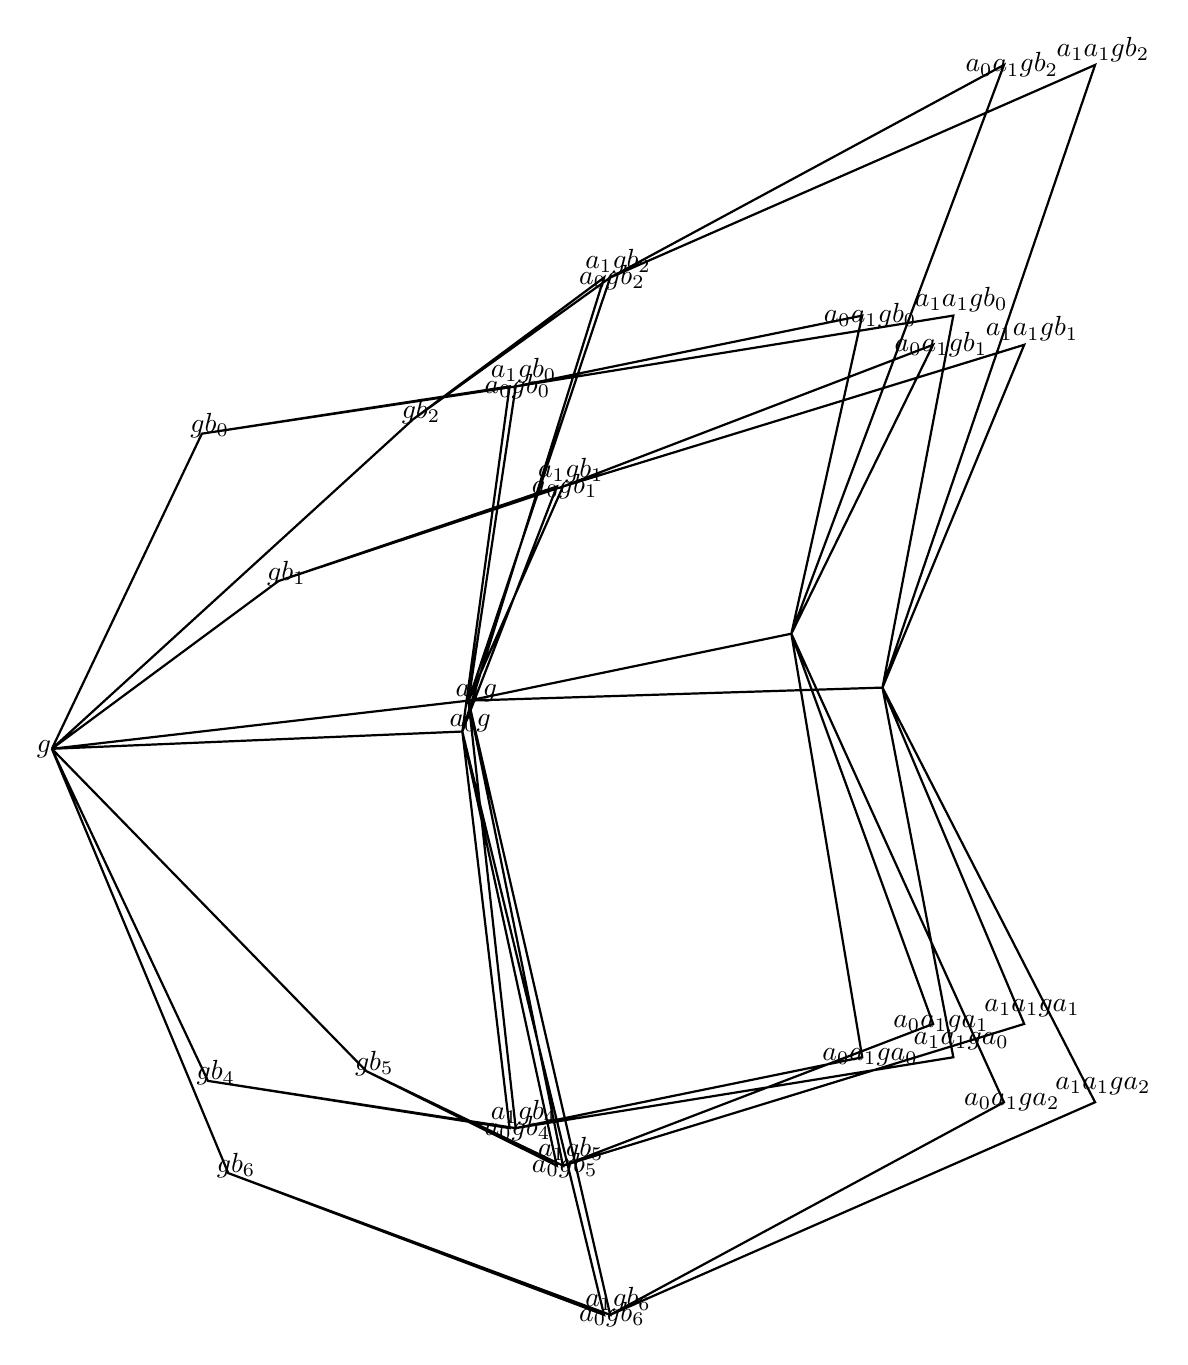
\begin{tikzpicture}
            \draw[thick](0,0)(0, 0) -- (1.9049911888377424,4.002079117547451) -- (5.81285084955138,4.602079117547451) -- (5.212850849551381,0.2192498173032679) -- (0, 0)
(0, 0) -- (2.879157898699928,2.130954290533681) -- (6.412850849551381,3.330954290533681) -- (5.212850849551381,0.2192498173032679) -- (0, 0)
(0, 0) -- (4.588270563356833,4.1850314105127575) -- (7.012850849551381,5.985031410512757) -- (5.212850849551381,0.2192498173032679) -- (0, 0)
(0, 0) -- (1.9049911888377424,4.002079117547451) -- (5.890590913653101,4.602079117547451) -- (5.2905909136531015,0.6119546131629411) -- (0, 0)
(0, 0) -- (2.879157898699928,2.130954290533681) -- (6.490590913653102,3.330954290533681) -- (5.2905909136531015,0.6119546131629411) -- (0, 0)
(0, 0) -- (4.588270563356833,4.1850314105127575) -- (7.090590913653101,5.985031410512757) -- (5.2905909136531015,0.6119546131629411) -- (0, 0)
(0, 0) -- (1.9818949186177792,-4.217396385887875) -- (5.81285084955138,-4.817396385887875) -- (5.212850849551381,0.2192498173032679) -- (0, 0)
(0, 0) -- (3.9944175473955323,-4.094159016671296) -- (6.412850849551381,-5.294159016671296) -- (5.212850849551381,0.2192498173032679) -- (0, 0)
(0, 0) -- (2.2401823432002748,-5.388664191428558) -- (7.012850849551381,-7.188664191428558) -- (5.212850849551381,0.2192498173032679) -- (0, 0)
(0, 0) -- (1.9818949186177792,-4.217396385887875) -- (5.890590913653101,-4.817396385887875) -- (5.2905909136531015,0.6119546131629411) -- (0, 0)
(0, 0) -- (3.9944175473955323,-4.094159016671296) -- (6.490590913653102,-5.294159016671296) -- (5.2905909136531015,0.6119546131629411) -- (0, 0)
(0, 0) -- (2.2401823432002748,-5.388664191428558) -- (7.090590913653101,-7.188664191428558) -- (5.2905909136531015,0.6119546131629411) -- (0, 0)
(5.2905909136531015, 0.6119546131629411) -- (5.890590913653101,4.602079117547451) -- (10.291575076901802,5.502079117547451) -- (9.391575076901802,1.4619219538089987) -- (5.2905909136531015, 0.6119546131629411)
(5.2905909136531015, 0.6119546131629411) -- (6.490590913653102,3.330954290533681) -- (11.191575076901803,5.130954290533681) -- (9.391575076901802,1.4619219538089987) -- (5.2905909136531015, 0.6119546131629411)
(5.2905909136531015, 0.6119546131629411) -- (7.090590913653101,5.985031410512757) -- (12.091575076901801,8.685031410512757) -- (9.391575076901802,1.4619219538089987) -- (5.2905909136531015, 0.6119546131629411)
(5.2905909136531015, 0.6119546131629411) -- (5.890590913653101,4.602079117547451) -- (11.4486392380322,5.502079117547451) -- (10.5486392380322,0.7771825477033486) -- (5.2905909136531015, 0.6119546131629411)
(5.2905909136531015, 0.6119546131629411) -- (6.490590913653102,3.330954290533681) -- (12.3486392380322,5.130954290533681) -- (10.5486392380322,0.7771825477033486) -- (5.2905909136531015, 0.6119546131629411)
(5.2905909136531015, 0.6119546131629411) -- (7.090590913653101,5.985031410512757) -- (13.248639238032201,8.685031410512757) -- (10.5486392380322,0.7771825477033486) -- (5.2905909136531015, 0.6119546131629411)
(5.2905909136531015, 0.6119546131629411) -- (5.890590913653101,-4.817396385887875) -- (10.291575076901802,-3.917396385887875) -- (9.391575076901802,1.4619219538089987) -- (5.2905909136531015, 0.6119546131629411)
(5.2905909136531015, 0.6119546131629411) -- (6.490590913653102,-5.294159016671296) -- (11.191575076901803,-3.494159016671296) -- (9.391575076901802,1.4619219538089987) -- (5.2905909136531015, 0.6119546131629411)
(5.2905909136531015, 0.6119546131629411) -- (7.090590913653101,-7.188664191428558) -- (12.091575076901801,-4.488664191428557) -- (9.391575076901802,1.4619219538089987) -- (5.2905909136531015, 0.6119546131629411)
(5.2905909136531015, 0.6119546131629411) -- (5.890590913653101,-4.817396385887875) -- (11.4486392380322,-3.917396385887875) -- (10.5486392380322,0.7771825477033486) -- (5.2905909136531015, 0.6119546131629411)
(5.2905909136531015, 0.6119546131629411) -- (6.490590913653102,-5.294159016671296) -- (12.3486392380322,-3.494159016671296) -- (10.5486392380322,0.7771825477033486) -- (5.2905909136531015, 0.6119546131629411)
(5.2905909136531015, 0.6119546131629411) -- (7.090590913653101,-7.188664191428558) -- (13.248639238032201,-4.488664191428557) -- (10.5486392380322,0.7771825477033486) -- (5.2905909136531015, 0.6119546131629411)
;
\node at (5.91285084955138,4.602079117547451) {$ a_{ 0  } gb_{ 0 } $};
\node at (6.512850849551381,3.330954290533681) {$ a_{ 0  } gb_{ 1 } $};
\node at (7.11285084955138,5.985031410512757) {$ a_{ 0  } gb_{ 2 } $};
\node at (5.990590913653101,4.802079117547451) {$ a_{ 1  } gb_{ 0 } $};
\node at (6.590590913653101,3.530954290533681) {$ a_{ 1  } gb_{ 1 } $};
\node at (7.190590913653101,6.1850314105127575) {$ a_{ 1  } gb_{ 2 } $};
\node at (5.91285084955138,-4.817396385887875) {$ a_{ 0  } gb_{ 4 } $};
\node at (6.512850849551381,-5.294159016671296) {$ a_{ 0  } gb_{ 5 } $};
\node at (7.11285084955138,-7.188664191428558) {$ a_{ 0  } gb_{ 6 } $};
\node at (5.990590913653101,-4.617396385887875) {$ a_{ 1  } gb_{ 4 } $};
\node at (6.590590913653101,-5.094159016671296) {$ a_{ 1  } gb_{ 5 } $};
\node at (7.190590913653101,-6.988664191428557) {$ a_{ 1  } gb_{ 6 } $};
\node at (10.391575076901802,5.502079117547451) {$ a_{ 0  } a_{ 1 }gb_{ 0 } $};
\node at (11.291575076901802,5.130954290533681) {$ a_{ 0  } a_{ 1 }gb_{ 1 } $};
\node at (12.1915750769018,8.685031410512757) {$ a_{ 0  } a_{ 1 }gb_{ 2 } $};
\node at (11.5486392380322,5.702079117547451) {$ a_{ 1  } a_{ 1 }gb_{ 0 } $};
\node at (12.4486392380322,5.330954290533681) {$ a_{ 1  } a_{ 1 }gb_{ 1 } $};
\node at (13.3486392380322,8.885031410512756) {$ a_{ 1  } a_{ 1 }gb_{ 2 } $};
\node at (10.391575076901802,-3.917396385887875) {$ a_{ 0  } a_{ 1 }ga_{ 0 } $};
\node at (11.291575076901802,-3.494159016671296) {$ a_{ 0  } a_{ 1 }ga_{ 1 } $};
\node at (12.1915750769018,-4.488664191428557) {$ a_{ 0  } a_{ 1 }ga_{ 2 } $};
\node at (11.5486392380322,-3.717396385887875) {$ a_{ 1  } a_{ 1 }ga_{ 0 } $};
\node at (12.4486392380322,-3.294159016671296) {$ a_{ 1  } a_{ 1 }ga_{ 1 } $};
\node at (13.3486392380322,-4.288664191428557) {$ a_{ 1  } a_{ 1 }ga_{ 2 } $};
\node at (-0.1,0) {$ g $};
\node at (5.31285084955138,0.3192498173032679) {$ a_{ 0 }g $};
\node at (5.390590913653101,0.7119546131629411) {$ a_{ 1 }g $};
\node at (2.0049911888377423,4.102079117547451) {$ gb_{ 0 } $};
\node at (2.979157898699928,2.230954290533681) {$ gb_{ 1 } $};
\node at (4.6882705633568325,4.285031410512757) {$ gb_{ 2 } $};
\node at (2.0818949186177793,-4.117396385887876) {$ gb_{ 4 } $};
\node at (4.094417547395532,-3.9941590166712957) {$ gb_{ 5 } $};
\node at (2.340182343200275,-5.288664191428558) {$ gb_{ 6 } $};          
\end{tikzpicture}
\end{center}

            \caption{Local environment of a square complex.}
            \label{fig:square}
           
            \end{figure}

Now we can state formally the theorem: 

\begin{theorem}
  For $\varepsilon \in \left( 0,\frac{1}{2} \right)$, $\gamma\in \left( \frac{1}{2} + \varepsilon, 1 \right)$, $\delta_{0}> 0$, large enough $\Delta$, and small codes $C_{A},C_{B}$ with distance at least $\delta_{0}\Delta$ if the dual tensor code of $C_{A},C_{B}$ is $w$-robust and $\Delta^{\gamma}$ resistance to puncturing, then there exists an infinite family of square complexes for which the Tanner code defined by the complexes and the dual tensor code such that any codeword with weigh less than $ \frac{\delta_{0}}{4\Delta^{3/2 + \varepsilon}} \cdot n \Delta^{2} $ is reducible \cref{ire}.
\end{theorem}

\begin{claim}
  Consider a codeword $c$ such there exists a negative vertex $v$ that adjoins only for normal vertices. Then $c$ is reducible, and there exits $y \in C_{A}^{\perp}\otimes C_{B}^{\perp}$ such that $y$ supported only on $v$ and $ | c_{v} + y | < |c_{v}| $.       
\end{claim}

\begin{proof}
 % Any row in the local view of $v$ can be thought as a codeword of $C_{B}$ plus faults made by adding $C_{A}\otimes \mathbb{F}_{2}$ to the corresponding sibling of $v$ regarding the row. As the dual tensor is $\Delta^{3/2+\varepsilon}$ robust. Then, \cite{kalachev2022twosided}       
\end{proof}




\begin{claim}
  The distance of the dual tensor code is at least $\delta\Delta$.
\end{claim}
\begin{proof}
By the robustness property, any codeword of the dual tensor code with a weight less than $\delta_{0}\Delta$ is supported on at most one row. Let $c$ be such a codeword and denote by $i$ the number of the non-trivial row. Fix a $c^{\prime} \in C_{A}^{\perp}$ such that the $i$th coordinate of  $c^{\prime}$ is non-zero and consider the multiplication of $c$ with the codewords of $C_{A}^\perp \otimes C_{B}^\perp$ of the following form:
  \begin{equation*}
    \begin{split}
      J = \left\{ c^{\prime} \otimes c_{b} : c_{b}\in C_{B}^{\perp} \right\} 
    \end{split}
  \end{equation*}
  So the $i$th row of any $x \in J$ is a codeword of $C_{B}^{\perp}$ and in total, collecting all the $i$th rows of codewords in $J$ sums up to all the code words in $C_{B}^{\perp}$. On the other hand, $c\cdot x = 0$ for all $x \in J$; that is, $c\cdot x = c_{i} \cdot c_{b} = 0$. Thus we obtain that $c_{i} \in C_{B}$ and therefore $|c_{i}| \ge \delta_{0}\Delta \Rightarrow |c| \ge \delta_{0}\Delta$, which is a contradiction.
\end{proof}

Denote by $S$ and $S_{-}$ the positive and negetive vertices support the codeword $x \in C_{x}$.
\begin{definition}
  Denote by $S_e$ and $S_n$ the exceptional and normal vertices, respectively, defined as follows: the weight of the local view for any vertex in $S_e$ is greater than $\Delta^{3/2 + \varepsilon}$, and $S_n$ is the complementary set of vertices. An edge in $G$ will be said heviy if it support more than $\Delta\delta - \frac{\Delta^{\frac{1}{2} + \varepsilon}}{\delta}$ squares in $G$. Denote by $T$ the  \ctt{complete definition}. In addition, denote by $T_s \subset T$ the vertices in $S_-$ that are surrounded by only normal vertices. Finally, for any pair of vertices subset $A,B$ such that $A \subset V^{+}$ and $B \subset V^{-}$ we denote the average heavy edges leaving out from $B$ to $A$ by $d_{B\rightarrow A}$.  
\end{definition}
\begin{claim}
  \label{claim:epss}
  for any $\varepsilon \in \left( 0,1 \right)$ and large enough $\Delta$  it holds that $ |S| \le \Delta^{\varepsilon}|S_{-}| $ 
\end{claim}
\begin{proof}
  Suppose not, namely that $|S| > \Delta^{\varepsilon}|S_{-}|$, then $|x|/|S_{-}| > \Delta^{\varepsilon}|x|/|S| > \Delta^{\varepsilon} \cdot \delta_{0}\Delta $ But:  
\begin{equation*}
  \begin{split}
    \frac{|x|}{|S_{-}|} = \frac{\Theta \left(E(S_{-},S_{-}) \right)}{|S_{-}|} \le \Theta(\Delta^{2})\frac{|S_{-}|}{n}  + \Theta(\Delta)  \rightarrow_{n\rightarrow \infty} \Theta(\Delta)
  \end{split}
\end{equation*}
\end{proof}

\begin{claim}
  \label{claim:portion}
  At least $ 1- \Delta^{-\frac{\varepsilon}{4}}$ portion of the negative vertices adjoin to only normal vertices. 
\end{claim}
% Define the graph $G^{\star} = (V_{-}, E^{\star})$ such that $E^{\star} = E \cup \left\{ \left\{g, xyg \right\} x\neq y, \in A\cup B \right\}$ And notice that the assumption follows that  any 
\begin{proof}
  Suppose through contradiction that for $\Delta^{-p}$ portion of the negative vertices $v_{-}\in V_{-}$ have at least one ($\Delta^{\gamma}$) sibling in $S_{e}$. Therefore $ \Delta^{-p} |S_{-}| \le \Delta |S_{e}|$ combining with \cref{claim:epss} it follows that $|S| \le \Delta^{1+\varepsilon + p }|S_{e}|$ : 
  \begin{equation*}
    \begin{split}
      \Delta^{3/2 + \varepsilon} & \le \frac{E(S,S_{e})}{|S_{e}|} = \Theta\left( \Delta^{2} \right)\frac{|S|}{n} + \Theta\left( \Delta \right)\sqrt{ \frac{|S|}{|S_{e}|}  }\\ 
      & \le \Theta(\Delta^{2}) \frac{|S|}{n} + \Theta(\Delta) \Theta\left( \Delta^{\frac{1+\varepsilon + p}{2}} \right)  
    \end{split}
  \end{equation*} 
  Thus we obtain contradiction for any $p < \varepsilon/2$. In particular for $p = \varepsilon/4$ we obtain that at least $1 - \Delta^{-\varepsilon/4}$ portion of the negative vertices are surounded by only normal vertices. 
 \end{proof}

 % \begin{claim}
%   Any $x \in \duC$ such that $|x| \le w$, and denote by $A^{\prime},B^{\prime}$ the rows and cols support $x$. Then $x$ can decompise into a sum of $x = t + s$ such that $t \in C_{A}\otimes \mathbb{F}^{B^\prime}$ and $s \in  \mathbb{F}^{A^\prime} \otimes  C_{B}$. 
% \end{claim}
% \begin{proof}
%   By induction on the number of raws supported $x$. Denote $x$ by 
%
%   \begin{equation*}
%     \begin{split}
%       x & = \sum_{i, c_{a}}{ c_{a} \otimes e_{i}  } + \sum_{i, c_{b} }{ e_{i} \otimes c_{b}} \\
%       & =  c_{a^{\prime}} \otimes e_{\tau} + \sum_{i / \tau, c_{a}}{ c_{a} \otimes e_{i}  } + \sum_{i, c_{b} }{ e_{i} \otimes c_{b}} \\
%      \end{split}
%   \end{equation*} 
%   
%   Now, if $c_{a^{\prime}} \otimes e_{\tau}$ decrese the summation weight then it must holds that $x$  
%
%    \begin{equation*}
%     \begin{split}
%       & =  c_{a^{\prime}} \otimes e_{\tau} + t^{\prime} + s^{\prime} = \overbrace{\left( c_{a^{\prime}} \otimes e_{\tau} + t^{\prime} \right) }^{ C_{A} \otimes \mathbb{F}^{B^{\prime}}}+ s^{\prime}
%     \end{split}
%   \end{equation*}
% \end{proof}
% 
 \begin{claim}  
   \label{claim:close}
   Let $x$ be a codeword of $\duC$ and $\xi < w$ such that $d(x, \mathbb{F}^{A} \otimes C_{B}) + d(x, C_{A}\otimes\mathbb{F}^{B}) \le \xi $ . Then $d(x, C_{A} \otimes C_{B}) < 3\xi $. 
 \end{claim} 
 \begin{proof}
Denote by $R$ the closest codeword of $C_{A}\otimes\mathbb{F}^{B}$ to $x$. Similarly, denote by $C$ the closest codeword of $\mathbb{F}^{A} \otimes C_{B}$ to $x$. Notice that $C + R \in \duC$. In addition, the weight of $C+R$ is bounded by:
   \begin{equation*}
     \begin{split}
       |R + C| &=  |x + \left(x + R\right) + x + \left( x + C\right)| \\
       & \le |\left(x + R\right)|+ |\left( x + C\right)| \le d\left( x ,   C_{A}\otimes\mathbb{F}^{B} \right) +  d\left( x ,   \mathbb{F}^{A} \otimes C_{B} \right) \\ 
       & \le w
     \end{split}
   \end{equation*}
   Therefore, by the robustness property, there are $r \in C_{A}\otimes\mathbb{F}^{B}$ and $c \in \mathbb{F}^{A} \otimes C_{B} $ such that $ R + C  = r + c$. And $r,c$ are supported on at most $|R+C|/\delta\Delta$ rows and columns. (Here $r$ and $c$ play the role of $s,t$ in \cref{def:wrobust}.)  

   Now observe that on one hand $C + c = R + r$, and on the other hand $ C + c \in \mathbb{F}^{A} \otimes C_{B} $ and $R+r \in C_{A}\otimes\mathbb{F}^{B}$. Therefore, $C+c \in C_{A}\otimes\mathbb{F}^{B} \cap \mathbb{F}^{A} \otimes C_{B}$. Namely, $C +c \in C_{A} \otimes C_{B}$. Thus we have:  
   
   \begin{equation*}
     \begin{split}
       d\left(x, C_{A}\otimes C_{B}\right) & \le d\left(x, C\right) + d\left(C, C_{A}\otimes C_{B} \right) \\
       &\le \xi + |c|
     \end{split}
   \end{equation*}
   And in the same way we obtain also that $d\left( x, C_{A} \otimes C_{B} \right) \le \xi + |r|$. Since $c,r$ are supported on at most $|R+C|/\delta\Delta$ rows and columns, the weight of the string obtained by joining a single row of $r$ with $c$ grows by at least $\delta\Delta - |R+C|/\delta\Delta > 0$. Therefore, $|c| < |c + r| = |R + C|$. Thus, in total, $d\left( x, C_{A} \otimes C_{B} \right) \le 3\xi$.
 \end{proof}

\begin{claim}
  \label{claim:closeto}
  Suppose that $v \in T_{s}$, Namely $v$ is surounded by only normal vertices. Then:
  \begin{equation*}
    \begin{split}
      d\left( c_{v}, C_{A}\otimes C_{B}\right) < \Theta\left( \Delta^{3/2+\varepsilon} \right)
    \end{split}
  \end{equation*} 
 \end{claim}
\begin{proof}
  By being surrounded only by normal vertices any row in the local view of $v$ is codeword of $C_{A}$ plus at most $\Delta^{3/2 + \varepsilon}/\Delta = \Delta^{\frac{1}{2}+\varepsilon}$ faults. So correcting the rows require flipping at most $\Delta \cdot \Delta^{\frac{1}{2} + \varepsilon}$ bits in total.  Thus $d\left(c_{v}, C_{A}\otimes \mathbb{F}^{B}\right) < \Delta^{3/2 + \varepsilon}$. In same way we obtain that $d\left(c_{v},  \mathbb{F}^{A} \otimes C_{B}\right) < \Delta^{3/2 + \varepsilon}$. Noitce that, in parituclar, $d(c_{v}, \duC) \le \Delta^{3/2 + \varepsilon}$.

  Denote by $y$ the closest codeword of $\duC$ to $c_{v}$. And observes that the distance between $y$ to either $C_{A} \otimes \mathbb{F}^{B}$ or $\mathbb{F}^{A}\otimes C_{B}$ is at most $2 \cdot \Delta^{3/2 + \varepsilon}$. To see it consider the decoding: 
  \begin{equation*}
    \begin{split}
  y \rightarrow x \rightarrow C_{A} \otimes \mathbb{F}^{B}   
    \end{split}
  \end{equation*}
  
  Therefore form \cref{claim:close} it follows that $d\left(y, C_{A} \otimes C_{B}\right) < 3 \xi $, So $d\left(x, C_{A} \otimes C_{B}\right) < \Delta^{3/2 + \varepsilon} +  3 \xi $.
     \end{proof}
   
   
 
 \begin{claim}[The Technical Lemma]  
   \label{cliam:tech} Let $A \subset S$ and $B \subset S_{-}$ subsets of the positive and the negetive vertices support $x$, and $\alpha \le \Delta^{2},\beta \le \Delta$ their minimal degrees in $G, G$. Assume the following conditions hold:
   \begin{enumerate}
     \item $\beta = \frac{\delta}{4 \sqrt{\Delta}}\alpha + \Theta\left(  \right)$
     \item Any vertex in $B$ has at least one heavily-siblinged vertex in $\bar{A}$.
   \end{enumerate}
   Then: $d_{B\rightarrow \bar{A}} = \Omega\left( \Delta \right)$.  
 \end{claim}

 \begin{proof}
   By the given $|S| \le \frac{2|x|}{\delta\Delta} \le \zeta\frac{2n\Delta}{\delta}$ we have that $|S|/n \le \zeta\cdot \frac{2\Delta}{\delta}$.
   %Let $A \subset S$ and $B \subset S_{-}$ subsets of the positive and the negetive vertices support $x$, and $\alpha \le \Delta^{2},\beta \le \Delta$ their minimal degrees in $G, G$.
   Then by the Mixing Expander Lemma we have that:   
   \begin{equation*}
     \begin{split}
       \alpha |A| & \le |E(A,S)| \le \frac{\Delta^{2}}{n}|A||S| + 4 \Delta \sqrt{|A||S|} \le |A| \cdot \zeta \frac{2\Delta^{3}}{\delta} +  4 \Delta \sqrt{|A||S|}\\ 
       & \Rightarrow \sqrt{|A|}\left(\alpha-\zeta \frac{2\Delta^{3}}{\delta}  \right) \le 4\Delta\sqrt{|S|} \\
       & \Rightarrow |A| \le \left( \alpha -  \zeta \frac{2\Delta^{3}}{\delta}  \right)^{-2} \cdot 16\Delta^{2}|S|
     \end{split}
   \end{equation*}
   And by repetting the same calculation but consider $B$ in the $G$ graph we obtain: 
\begin{equation*}
     \begin{split}
       \Rightarrow  |B| \le & \left( \beta -  \zeta \frac{4 \cdot 2\Delta^{2} }{\delta}  \right)^{-2} \cdot 16\Delta|S|\\
       \Rightarrow  |B| \le & \left( \frac{\delta}{\sqrt{\Delta}}\alpha   -  \zeta \frac{4 \cdot 2\Delta^{2} }{\delta}  \right)^{-2} \cdot 16\Delta|S|\\
       = & \frac{\Delta}{\delta^{2}} \left(  \alpha -  4\cdot 2\zeta \frac{\Delta^{2\frac{1}{2}}}{\delta^{2}}   \right)^{-2} \cdot 16\Delta|S| 
     \end{split}
   \end{equation*}
   And for large enugh $\Delta$ the above is bounded by:
   \begin{equation*}
     \begin{split}
     \left(  \alpha -  4\cdot 2\zeta \frac{\Delta^{2\frac{1}{2}}}{\delta^{2}}   \right) \ge \left( \alpha -  \zeta \frac{2\Delta^{3}}{\delta}  \right) \Rightarrow |B|  \le  & \frac{1}{\delta^{2}} \left( \alpha -  \zeta \frac{2\Delta^{3}}{\delta}  \right)^{-2} \cdot 16\Delta^{2}|S| 
     \end{split}
   \end{equation*}
   Now, choose $\zeta$ such $\left( \alpha -  \zeta \frac{2\Delta^{3}}{\delta}  \right) \ge 16^{\frac{1}{2}} \cdot 100 \Delta^{1\frac{1}{2}}$ yields that: $|A| \le 10^{-4}\Delta^{-1} |S| \Rightarrow $$ |\bar{A}| \ge \left( 1 - 10^{-4} \Delta^{-1}\right)|S|$, And $|B| \le 10^{-4} \frac{|S|}{16 \delta^{2}\Delta}$. Hence:

   \begin{equation*}
     \begin{split}
       d_{B\rightarrow \bar{A}} = \frac{ E\left(B,\bar{A}\right) }{|B|} \ge \frac{|\bar{A}|}{|B|} \ge \left( 1 - 10^{-4}\Delta^{-1}  \right) 10^{4} \cdot \delta^{2}\Delta  = \Theta\left( \Delta \right)
     \end{split}
   \end{equation*}
 \end{proof}
 
 \begin{claim}
   \label{claim:satis}
   $S_{e}$ and $T$ satisfies the requrirments of \cref{cliam:tech} with $A = S_{e}$, $B = T$, $\alpha = \Delta^{3/2 + \varepsilon}$ and $\beta = \Delta\delta + \Delta^{\frac{1}{2} + \varepsilon}$. That is, the average of havey edges form $T$ to $S_{n}$ is $\Theta\left( \Delta \right)$. 
 \end{claim}

 \begin{proof}
 \end{proof}

\begin{claim}
  \label{claim:linear}
  There is a normal-surounded vertex in $v \in T_{s}$ in weight at least $\Theta\left(\Delta^{2}\right)$.   
 \end{claim}
 \begin{proof}
   We know from \cref{claim:satis} that $d_{T\rightarrow S_{n} }$ is linear in $\Delta$. Morever \cref{claim:portion} tell us that most of the vertices in $S_{-}$ are surrounded only by normal vertices. Denote by $\expp{ d(v) | v \in T_{s} }$ the expected degree of heavy edges connected to vertex in $T_{s}$. Using the conditional expection formula we get:
  
   \begin{equation*}
     \begin{split}
       d_{T \rightarrow S_{n}} &= \expp{ d(v) | v \in T_{s} } \prb{ v \in T_{s}} + \expp{d\left( v \right) | v \in T / T_{s}} \prb{ v \in T / T_{s}} \\
       & \le \expp{ d(v) | v \in T_{s} } \prb{ v \in T_{s}} + \expp{d\left( v \right) | v \in T / T_{s}} \prb{ v \in S_{-} / T_{s}} \\
       & \le \expp{ d(v) | v \in T_{s} } \cdot 1   + \Delta \cdot  \Delta^{-\varepsilon/4} \\
       & \Rightarrow  \expp{ d(v) | v \in T_{s} } \ge d_{T \rightarrow S_{n}} - \Delta^{\frac{3}{4} \varepsilon} = \Theta\left( \Delta \right) 
     \end{split}
   \end{equation*}
   Therefore there is at least a single vertex in $T_{s}$ connected to $\Theta\left( \Delta \right)$ havey edges. Combining the fact that edge is heavy edge if there are at least $\Delta\delta - \Delta^{\frac{1}{2} + \varepsilon}$ non trival bits on it's squares we get the desired.  
 \end{proof}

 We are about to finish the proof of the theorem. Combining \cref{claim:linear} and \cref{claim:closeto} we obtain the the existnes of a negative vertex which is both at distance $\Theta\left(\Delta^{3/2 + \varepsilon}\right)$ form $C_{A}\otimes C_{B}$ and weight at least $\Theta\left( \Delta^{2} \right)$. Denote by $v \in T_{s}$ that vertex, by $c_{v}$ it's local view and by $y \in C_{A}\otimes C_{B}$ the closest codeword to $c_{v}$. Subtructing $y$ from $c_{v}$ yilds: 
 
 \begin{equation*}
   \begin{split}
     \left|   c_{v} + y   \right| &= d\left( c_{v}, y  \right) = \Theta\left( \Delta^{3/2 + \varepsilon} \right) < \left|   c_{v}   \right|     \\
     \Rightarrow & | c + y| < |c| 
   \end{split}
 \end{equation*}

 \section{LTC.}

\begin{definition}[The Disagreement Code] Given a Tanner code $C = \Tann$, define the code $C_{\oplus}$ to contain all the words equal to the formal summation $ \sum_{v \in V\left( G \right)} {c_{v} }$ when $c_{v}$ is an assignment of a codeword $ c_{v} \in C_0 $  on the edges of the vertex $ v \in V\left( G \right)$.
  We call to such code the \textbf{disagreement code} of $C$, as edges are set to 1 only if their connected vertices contribute to the summation codewords that are different on the corresponding bit to that edge. In addition, we will call to any contribute $c_v$, the \textbf{suggestion} of $v$. And notice that by linearity, each vertex suggests, at most, a single suggestion.   

  Finally, given a bits assessment $x \in \mathbb{F}_{2}^{E}$ over the edges of $G$, we will denote by $x^{\oplus} \in C_{\oplus} $ the codeword which obtained by summing up suggestions set such each vertex suggests the closet codeword to his local view. Namely, for each $v \in V$ define:   
  \begin{equation*}
    \begin{split}
      c_{v} & \leftarrow \arg_{ \tilde{c} \in C_{0}} \min{ d( x|_{v} , \tilde{c} ) } \ \ \forall v\in V   \\
      x^{\oplus} & \leftarrow \sum_{v \in V}{c_{v}} 
    \end{split}
  \end{equation*}
  We will think about $x^{\oplus}$ as the disagreement between the vertices over $x$. 

\end{definition}

\begin{definition} Let $C = \Tann$. We say that $x \in C_{\oplus}$ is \textbf{reducible} if there exists a vertex $v$ and a small codeword $c_v$, for which, adding the assignment of $c_v$ over the $v$'s edges to $x$ decreases the weight. Namely, $|x + c_{v}| < |x|$. If $x \in C_{\oplus}$ is not a reducible codeword then we say that $x$ is \textbf{irreducible} \label{ire}. \end{definition}

The following lemma states that the disagreement is invariant when adding codewords, resulting in any decoder that can correct errors occurring to the trivial codeword by taking the derived disagreement as input being able to correct the same errors when they occur to any codeword.

\begin{lemma}[Linearity of The Disagreement] \label{lemma:lin} Consider the code $C = \Tann$. Let $ x \in \mathbb{F}_{2}^{E}$ then for any $ y \in C$ it holds that: 
  \begin{equation*}
    \begin{split}
      \left( x + y  \right)^{\oplus} = \left( x  \right)^{\oplus} 
    \end{split}
  \end{equation*}
\end{lemma}
  \begin{proof} Having that $y \in C$ followes $y|_v \in C_{0}$ and therefore 


    \begin{equation*}
      \begin{split}
        \arg_{ \tilde{c} \in C_{0}} \min{ d( z  , \tilde{c} ) } = y|_{v} + \arg_{ \tilde{c} \in C_{0}} \min{ d( z, \tilde{c} + y|_{v} ) } 
      \end{split}
    \end{equation*}
     Hence the suggestion made by vertrx $v$ is: 
  \begin{equation*}
    \begin{split}
      c_{v}\leftarrow &  \arg_{ \tilde{c} \in C_{0}} \min{ d( (x+y)|_{v}  , \tilde{c} ) } \\
      \leftarrow &  y|_{v} +  \arg_{ \tilde{c} \in C_{0}} \min{ d( (x+y)|_{v}  , \tilde{c} + y|_{v} ) } \\
      \leftarrow &  y|_{v} +  \arg_{ \tilde{c} \in C_{0}} \min{ d( x|_{v} , \tilde{c} ) } 
    \end{split}
  \end{equation*}
  It follows that: 

  \begin{equation*}
    \begin{split}
      \left( x + y \right)^{\oplus} =& \sum_{v\in V}{c_{v}} = \sum_{v \in V}{y|_{v}} + \sum_{v\in V}{ \arg_{ \tilde{c} \in C_{0}} \min{ d( x|_{v} , \tilde{c} ) } } \\ 
      =& y^{\oplus} + x^{\oplus} = x^{\oplus}
    \end{split}
  \end{equation*}
  When the last transition follows immediately by the fact that $y \in C$ and therefore any pair of connected vertices contribute the same value for their associated edge \end{proof}
%
%  \begin{definition} Let $C = \Tann$. We say that $x \in C_{\oplus}$ is \textbf{reducable} if there exists a vertex $v$ and a small codeword $c_v$, for which, adding the assignment of $c_v$ over the $v$'s edges to $x$ decreases the weight. Namely, $|x + c_{v}| < |x|$. If $x \in C_{\oplus}$ is not a reducable codeword then we say that $x$ is \textbf{ireducable} \label{ire}. \end{definition}
%
%


\section{Decoding and Testing}
  For completeness, we show exactly how Theorem 1 implies testability. The following section repeats Leiverar's and Zemor's proof \cite{leverrier2022quantum}. Consider a binary string $x$ that is not a codeword. The main idea is the observation that the number of bits filliped by (any) decoder, while decoding $x$, bounds the distance $d\left( x, C \right)$ from above. In addition, the number of positive checks in the first iteration is exactly the number of violated restrictions.
%\begin{figure*}[h]
%\begin{adjustbox}{width=\textwidth}
  \begin{definition}Let $L = \{L_{i}\}^{2|E|}_{0}$  be a series of $2|E|$. Such that for each vertex $ v \in V$ $\sum_{ e = \{u,v\} }{ L_{e_v} } \in C_{0}$. We will call $L$ a \textit{Potential list} and refer to the $e_{v}$'the element of $L$ as a suggestion made by the vertex $v \in V$ for the edge $e \in E$. Sometimes we will use the notation $L_{v}$ to denote all the $L$'s coordinates of the form $ L_{e_{v}} \forall e \in \text{Support} \left( v \right) $. Define the \textit{Force} of $L$ to be the following sum $  F\left( L \right) = \sum_{e = \{v,u\} \in E }{ \left(L_{e_v} + L_{e_u}\right) }$ and notice that $ F\left( L \right) \in C_{\oplus}$. And define the \textit{state} $S(L) \subset \mathbb{F}^{|E|}_{2}$ of $L$ as the vector obtained by choosing an arbitrary value from $ \{ L_{e_v}, L_{e_u} \}$ for each edge $e \in E$.  
  \end{definition}
  \begin{claim} \label{claim:pot} Let $L$ be the Potential list. If $F(L)=0$ then $S(L)\in C$. \end{claim}
  \begin{proof} Denote by $\phi\left( e \right) \subset \{ L_{e_v}, L_{e_u} \}$ the value which was chosen to $e = \{v,u\} \in E$. By $F\left(L\right) = 0$ , it follows that $ L_{e_v} + L_{e_u} = 0 \Rightarrow L_{e_v} = L_{e_u} = \phi\left( e \right) $ for any $e \in E$. Hence for every $v\in V$ we have that $ S\left( L \right)|_{v} = \sum_{u \sim v}{ \phi\left( \{v,u\} \right) } =  \sum_{u \sim v}{ L_{e_v }} \in C_{0}$ $ \Rightarrow S\left( L \right) \in C$   
  \end{proof}
  The decoding goes as follows. First, each vertex suggests the closet $C_{0}$'s codeword to his local view. Those suggestions define a Potential list, denote it by $L$, then if $F\left( L \right) <\tau$, by Theorem 1, one could find a suggestion of vertex $v$ and a codeword $c_v$ such that updating the value of $L_{v} \leftarrow L_{v} + c_{v}$ yields a Potential list with lower force. Therefore repeating the process till the force vanishes, obtain a Potential list in which its state is a codeword. 
  \begin{definition} Let $\tau > 0, f : \mathbb{N} \rightarrow \mathbb{R^{+}}$, and consider a Tanner Code $C = \mathcal{T}\left( G, C_{0} \right)$. Let us Define the following decoder and denote it by $\mathcal{D}$.  
  \end{definition}

  \begin{algorithm}[h]
    \caption{Decoding}
    \label{alg:three}
    \KwData{ $x \in \mathbb{F}_{2}^{n}$ }
    \KwResult{ $\arg\min {\left\{  y \in C : |y + x|  \right\} }$ if $d(y,C) < \tau $ and False otherwise. }
    $ L \leftarrow \text{Array} \{ \} $\\
    \For { $ v \in V$} {
      $c^{\prime}_{v} \leftarrow \arg\min {\left\{  y \in C_{0} : |y + x|_{v} |  \right\} } $\\
      $ L_{v} \leftarrow c^{\prime}_{v}$
    }
    $ z \leftarrow \sum_{v \in V}{c^{\prime}_{v}} $\\
    \eIf{ $ |z| < \tau \frac{n}{f\left( n \right)} $}{
      \While{ $|z| > 0$ }{
	find $v$ and $c \in C_{0}$ such that $|z + c_{v}| < |z|$\\
	$z \leftarrow z + c_{v}$ \\
	$ L_{v} \leftarrow  L_{v} + c_{v}$
      }
    }{
      reject. 
    }
    \Return  $S(L) $

  \end{algorithm}

  \begin{theorem}
Consider a Tanner Code $C = [n, n\rho, n\delta]$ and the corresponding disagreement code $C_{\oplus}$. Suppose that for every codeword $z \in C_{\oplus}$ such that $|z| < \frac{\tau^{\prime} n}{f\left(n\right)}$, there exists a vertex $v$ and a suggestion for $v$ which is another codeword $y \in C_{\oplus}$ such that $|z + y| < |z|$. Set $\tau \leftarrow \frac{\tau^{\prime}}{6 \Delta} \delta$ then.

  \begin{enumerate}
    \item $\mathcal{D}$ corrects any error at a weight less than $\tau n / f\left(n\right)$.   
    \item $C$ is $f\left( n \right)$ testable code.
  \end{enumerate}
\end{theorem}

\begin{proof} So it is clear from the claim \cref{claim:pot} above that if the condition at line (6) is satisfied, then $\mathcal{D}$  will converge into some codeword in $C$. Hence, to complete the first section, it left to show that $\mathcal{D}$ returns the closest codeword. Denote by $e$ the error, and by simple counting arguments; we have that $\mathcal{D}$ flips at most:  
  \begin{equation*}
    \begin{split}
      d_{\mathcal{D}}\left( x, C \right) & \le 2|e|\Delta + \tau \frac{n}{f\left( n \right)}\Delta
    \end{split}
  \end{equation*}
  bits. Hence, by the assumption, 
  \begin{equation*}
    \begin{split}
      d_{\mathcal{D}}\left( x, C \right) & \le 3\Delta \tau \frac{n}{f\left( n \right)} \le 3\Delta \tau\delta n < \frac{1}{2} \delta n  
    \end{split}
  \end{equation*}
  Therefore the code word returned by $\mathcal{D}$ must be the closet. Otherwise, it contradicts the fact that the relative distance of the code is $\delta$.
  To obtain the correctness of the second section, we will separate when the conditional at the line (5) holds and not. And prove that the testability inequality holds in both cases. 
  Let $x \in \mathbb{F}_{2}^{n}$ and consider the running of $\mathcal{D}$ over $x$. Assume the first case, in which the conditional at line (5) is satisfied. In that case, $\mathcal{D}$ decodes $x$ into its closest codeword in $C$. Therefore:
  \begin{equation*}
    \begin{split}
      d\left( x, C \right) \le & \ d_{D} \left( x, C \right) \le m\xi\left( x \right)\Delta +  |z|\Delta  \\ \le &  \  m\xi\left( x \right)\Delta + m\xi\left( x \right)  \Delta^{2} \\ 
      \frac{d\left( x, C \right)}{n} \le & \  \kappa_{1} \xi\left( x \right)    
    \end{split}
  \end{equation*}
  Now, consider the other case in which: $ |z| \ge \tau \frac{n}{f\left( n \right)}  $.
  \begin{equation*}
    \begin{split}
      \frac{d\left( x, C \right)}{n} & \le 1 \le \frac{|z|}{\tau n}f\left( n \right) \le \frac{m}{n} \frac{1}{\tau} \Delta \xi\left( x\right)f\left( n \right) \\ & \le \kappa_{2} \xi\left( x \right)f\left( n \right)  
    \end{split}
  \end{equation*}
  Picking $ \kappa \leftarrow \max \{ \kappa_{1}, \kappa_{2} \}$ proves $f\left( n \right)$-testability
\end{proof}



%\printbibliography[heading=subbibliography]


\chapter{Further Research.}
Both good quantum LDPC and good LTC had been open problems for more than decades, so the fact that they have been solved in one stroke raises two interesting questions. The first one is whether the construction that obtains each of them alone can also yield good quantum LTC? What is the exact challenge that prevents the inventors from proceeding into quantum testability?

The second question is whether one of the codes can be obtained without giving the other. Either positive or negative answers to these questions will shed light on our understanding of what quantumness is.

In this chapter, we present our attempts to provide answers. The chapter is divided into two parts. In the first, we demonstrate a variation of the classical Tanner code that defines many equations. We believe that this variation contains enough structure to guarantee degeneration of equations similarly to what occurs in the polynomial code. In the second chapter, we show that the polynomial code is not $w$-robust. If it were not the case, then one could hope to obtain quantum testability by considering a Tanner code in which any vertex restricts its local view to be a codeword of a quantum code.



\section{Local Majority $\neq$ Local Testability.}

We begin by demonstrating that selecting $C_0$, the small code in the Tanner code, to have a large distance, which can also be considered as adding numerous restrictions, yields testability. However, the amount one will have to enlarge the distance to cannot be achieved with a rate greater than $\frac{1}{2}$ by the Singleton bound.
  %\section{Construction}
  \subsection{Almost LTC With Zero Rate}
%  \begin{definition}[The Disagreement Code] Given a Tanner code $C = \Tann$, define the code $C_{\oplus}$ to contain all the words equal to the formal summation $ \sum_{v \in V\left( G \right)} {c_{v} }$ when $c_{v}$ is an assignment of a codeword $ c_{v} \in C_0 $  on the edges of the vertex $ v \in V\left( G \right)$.
  We call to such code the \textbf{disagreement code} of $C$, as edges are set to 1 only if their connected vertices contribute to the summation codewords that are different on the corresponding bit to that edge. In addition, we will call to any contribute $c_v$, the \textbf{suggestion} of $v$. And notice that by linearity, each vertex suggests, at most, a single suggestion.   

  Finally, given a bits assessment $x \in \mathbb{F}_{2}^{E}$ over the edges of $G$, we will denote by $x^{\oplus} \in C_{\oplus} $ the codeword which obtained by summing up suggestions set such each vertex suggests the closet codeword to his local view. Namely, for each $v \in V$ define:   
  \begin{equation*}
    \begin{split}
      c_{v} & \leftarrow \arg_{ \tilde{c} \in C_{0}} \min{ d( x|_{v} , \tilde{c} ) } \ \ \forall v\in V   \\
      x^{\oplus} & \leftarrow \sum_{v \in V}{c_{v}} 
    \end{split}
  \end{equation*}
  We will think about $x^{\oplus}$ as the disagreement between the vertices over $x$. 

\end{definition}

\begin{definition} Let $C = \Tann$. We say that $x \in C_{\oplus}$ is \textbf{reducible} if there exists a vertex $v$ and a small codeword $c_v$, for which, adding the assignment of $c_v$ over the $v$'s edges to $x$ decreases the weight. Namely, $|x + c_{v}| < |x|$. If $x \in C_{\oplus}$ is not a reducible codeword then we say that $x$ is \textbf{irreducible} \label{ire}. \end{definition}

The following lemma states that the disagreement is invariant when adding codewords, resulting in any decoder that can correct errors occurring to the trivial codeword by taking the derived disagreement as input being able to correct the same errors when they occur to any codeword.

\begin{lemma}[Linearity of The Disagreement] \label{lemma:lin} Consider the code $C = \Tann$. Let $ x \in \mathbb{F}_{2}^{E}$ then for any $ y \in C$ it holds that: 
  \begin{equation*}
    \begin{split}
      \left( x + y  \right)^{\oplus} = \left( x  \right)^{\oplus} 
    \end{split}
  \end{equation*}
\end{lemma}
  \begin{proof} Having that $y \in C$ followes $y|_v \in C_{0}$ and therefore 


    \begin{equation*}
      \begin{split}
        \arg_{ \tilde{c} \in C_{0}} \min{ d( z  , \tilde{c} ) } = y|_{v} + \arg_{ \tilde{c} \in C_{0}} \min{ d( z, \tilde{c} + y|_{v} ) } 
      \end{split}
    \end{equation*}
     Hence the suggestion made by vertrx $v$ is: 
  \begin{equation*}
    \begin{split}
      c_{v}\leftarrow &  \arg_{ \tilde{c} \in C_{0}} \min{ d( (x+y)|_{v}  , \tilde{c} ) } \\
      \leftarrow &  y|_{v} +  \arg_{ \tilde{c} \in C_{0}} \min{ d( (x+y)|_{v}  , \tilde{c} + y|_{v} ) } \\
      \leftarrow &  y|_{v} +  \arg_{ \tilde{c} \in C_{0}} \min{ d( x|_{v} , \tilde{c} ) } 
    \end{split}
  \end{equation*}
  It follows that: 

  \begin{equation*}
    \begin{split}
      \left( x + y \right)^{\oplus} =& \sum_{v\in V}{c_{v}} = \sum_{v \in V}{y|_{v}} + \sum_{v\in V}{ \arg_{ \tilde{c} \in C_{0}} \min{ d( x|_{v} , \tilde{c} ) } } \\ 
      =& y^{\oplus} + x^{\oplus} = x^{\oplus}
    \end{split}
  \end{equation*}
  When the last transition follows immediately by the fact that $y \in C$ and therefore any pair of connected vertices contribute the same value for their associated edge \end{proof}
%
%  \begin{definition} Let $C = \Tann$. We say that $x \in C_{\oplus}$ is \textbf{reducable} if there exists a vertex $v$ and a small codeword $c_v$, for which, adding the assignment of $c_v$ over the $v$'s edges to $x$ decreases the weight. Namely, $|x + c_{v}| < |x|$. If $x \in C_{\oplus}$ is not a reducable codeword then we say that $x$ is \textbf{ireducable} \label{ire}. \end{definition}
%
%


  \begin{theorem}[LTC Zero Rate] 
      \label{theorem:ltczerorate}
    There exist a constant $\alpha > 0$ and an infinte family of Tanner Codes $C = \Tann$ such that any \ireducable codeword $x$ of a coresponding disagreement code $x \in C_{\oplus}$ at length $n$, weight at least $\alpha n$. \end{theorem}



  \paragraph{Proof.} By induction over the number of vertices $V^\prime \subset V$, which suggest a nontrivial codeword to $x$. Base, assume that a single vertex $v \in V$ suggests a nontrivial codeword $c_{v} \in C_{0}$. Then it's clear that $x = c_{v}$. And therefore, we have that $|x +c_{v}| = 0 < |x|$.

  Assume the correctness of the argument for every codeword defined by at most $m$ nontrivial suggestions made by $V^\prime \subset V$. And consider the graph $\left( V^\prime, E^\prime \right)$ induced by them. If the graph has more than a single connectivity component, then any of them is also a codeword of $C_{\oplus}$  but composed of at most $m-1$ nontrivial suggestions. Therefore, by the assumption, we could find a vertex $v$ and a proper small codeword $c_v \in C_0 $, such that the addition of the suggestion will decrease the weight of the codeword defined on that component and therefore decrease the total weight of $x$.

  So, we can assume that the vertices in $V^\prime$ compose a single connectivity component. Let be $x|_{v} \in \mathbb{F}_{2}^{\Delta}$ the bits of $x$ on the indices corresponding to $v$'s edges. For any $S \subset E$, define $w_{S}\left( x \right)$ as the weight that $x$ induces over $S$. Sometimes we will refer to $w_{S}\left( x \right)$ as the \textbf{flux} induced by $x$ over $S$.

  The genreal idea of the proof is to show that if the distance of the small code is large ($ \ge \frac{2}{3}$ ) and $x$ is \ireducable codeword then there exist an indepandent subset of vertices $U \subset V^{\prime}$, at linear size, that induce a significant flux over $E/E^{\prime}$. If $U$ has linear size than also $x$ has a linear size, And if not, Then we will show that no serious interface has been occurred. ~\cref{claim:deg} and ~\cref{claim:tree-size} state that if one is willing to hide an ireducable \hyperref[ire]{[\ref{ire}]} error then he has to touch at least a linar number of verties. ~\cref{claim:flu1} and  ~\cref{claim:flu2} quanitify the flux that induced by such errors. 

\begin{claim}\label{claim:deg} For any $v \in V^\prime$ and corresponded suggestion $c_{v}$ it holds that: $w_{E^\prime}\left( c_{v} \right) \ge \frac{1}{2}\delta_{0}\Delta$. \end{claim}
  \begin{proof} Notice that any edge of $E$ connected only to a single vertex in $V^\prime$ equals the corresponding bit in the original suggestion made by $c_{v}$. Hence for every $v\in V^\prime$, it holds that: 
\begin{equation*}
      \begin{split}
	    w_{E / E^\prime}\left(x|_{v}\right) = w_{E / E^\prime}\left(c_{v}\right) \Rightarrow  w_{E / E^\prime}\left(x|_{v}\right) \le | x \cap c_{v} |
      \end{split}
    \end{equation*}
     Now consider the weight of $x + c_{v}$, By the assumption that $x$ is ireducable code word of $c_{\oplus}$ we have that: 
  
 \begin{equation*}
    \begin{split}
       |x + c_{v}| & = |x| + |c_{v}| - 2|x \cap c_{v}| > |x| \\
       \Rightarrow &   |x \cap c_{v}|  < \frac{1}{2} |c_{v}| \\
      w_{E^\prime}\left( c_{v} \right) &= |c_{v}| - w_{E / E^\prime}\left( c_{v} \right) =  |c_{v} | - w_{E / E^\prime}\left( x|_{v} \right) \\ 
      & \ge | c_{v} | - | x \cap c_{v} |  \ge \frac{1}{2}|c_{v}| = \frac{1}{2}\delta_{0}\Delta 
    \end{split}
  \end{equation*}
  \end{proof}

  Consider an arbitrary vertex $r \in V^\prime$, and consider the DAG obtained by the BFS walk over the subgraph $\left(V^\prime, E^\prime \right)$ starting at $r$. Denote this directed tree by $T$.

%Let $g$ be the girth of the graph and consider a layer $U$ in $T$ at height $h\left( U \right)$ satisfies the inequality $ h\left( U \right) < \frac{1}{2}g + l$ for some integer $l$.
  %\begin{adjustbox}{width=150pt}%\columnwidth}
%\begin{figure*}[t]%{width=150pt} %0.3\textwidth}

  
%\end{figure*}
%\end{adjustbox} 
  \begin{claim} \label{claim:tree-size} The size of $T$ is at least:
  \begin{equation*}
    \begin{split}
      |T| & \ge \left( \frac{1}{4}\delta_{0} - \frac{\lambda}{\Delta} \right)n 
    \end{split}
  \end{equation*}
\end{claim}
\begin{proof}By~\cref{claim:deg}  any $v \in T$ the degree of $v$ is at least $\frac{1}{2}\delta_{0}\Delta$ we have that: $E\left( T,T \right) \ge \frac{1}{2}\cdot \frac{1}{2}\delta_{0}\Delta |T|$. Combine the Mixining Expander Lemma we obtain:
  \begin{equation*}
    \begin{split}
      \frac{1}{4}\delta_{0}\Delta |T| & \le \frac{\Delta}{n}|T|^2  + \lambda|T| \\ 
      \Rightarrow & \left( \frac{\Delta}{n}|T| + \lambda -  \frac{1}{4}\delta_{0}\Delta \right)|T| \ge 0 \\ 
      \Rightarrow & |T| \ge \left( \frac{1}{4}\delta_{0} - \frac{\lambda}{\Delta} \right)n 
    \end{split}
  \end{equation*}
  \end{proof}



\begin{claim} \label{claim:flu1}  Suppose that $G$ is an expander graph with a second eigenvalue $\lambda$, then For any layer $U$ there exist a layer $U^{\prime}$ such that:
  \begin{equation*}
    \begin{split}
      (1) & \ \ |U^{\prime}| \ge |U| \\
      (2) & \ \ w_{E/E^{\prime}}\left( x|_{U^{\prime}} \right)  \ge\Delta|U^{\prime}|\left( \delta_{0}-\frac{2}{3}-\frac{2\lambda}{\Delta} \right)
    \end{split}
  \end{equation*}
\end{claim} 
  \begin{proof} Consider layer $U$ and denote by $U_{-1}$ and $U_{+1}$ the preceding and the following layers to $U$ in $T$. It follows from the expander mixing lemma that:
  \begin{equation*}
    \begin{split}
      w_{E/E^{\prime}}\left( x|_{U} \right) & \ge \delta_{0}\Delta|U| -\wcutUU \ge \\ 
      & \delta_{0}\Delta|U| - \cutUU \\ 
      &  \delta_{0}\Delta|U| - \Delta\frac{|U||U_{-1}|}{n} - \Delta\frac{|U||U_{+1}|}{n} \\
      & -\lambda\sqrt{|U||U_{-1}|} - \lambda\sqrt{|U||U_{+1}|}
    \end{split}
  \end{equation*}

  \begin{claim} \label{claim:maxu} We can assume that $|U| \ge |U_{-1}|, |U_{+1}|$. \end{claim}
  \begin{proof} Suppose that $|U_{+1}| > |U|$, so we could choose $U$ to be $U_{+1}$. Continuing stepping deeper till we have that $|U| > |U_{+1}|, |U_{-1}|$. Simiraly, if $|U| > |U_{+1}|$ but $|U_{-1}| > |U|$, the we could take steps upward by replacing $U_{-1}$ with $U$. At the end of the process, we will be left with $U$ at a size greater than the initial layer and $|U| > |U_{+1}|, |U_{-1}|$ \end{proof}

  Using ~\cref{claim:maxu}, we have that $\left( |U_{+1}| + |U_{-1}| \right)/n <\frac{2}{3} $ and therefore:
  \begin{equation*}
    \begin{split}
      w_{E/E^{\prime}}\left( x|_{U} \right) & \ge \left( \delta_{0} - \frac{2}{3} - \frac{2\lambda}{\Delta} \right) \Delta |U| \ \   
    \end{split}
  \end{equation*}
\end{proof}
  That immediately yields the following: let $U_{\text{max}} = \text{arg} \max_{U \text{ layer in }  T } |U|  $  then: 
  \begin{equation*}
    \begin{split}
      |x| \ge  w_{E/E^{\prime}}\left( x|_{U_{\text{max}}} \right) \ge \left( \delta_{0} - \frac{2}{3} - \frac{2\lambda}{\Delta} \right)\Delta |U_{\text{max}}|
    \end{split}
  \end{equation*}
  \begin{claim}  \label{claim:flu2}Consider again the maximal layer $U_{\max}$ then: 
  \begin{equation*}
    \begin{split}
      w_{E/E^{\prime}}\left( x \right) \ge \left( \delta_{0} - \frac{|U_{\max}|}{n} - \frac{\lambda}{\Delta} \right) \Delta|T| 
    \end{split}
  \end{equation*}
\end{claim}

  \begin{proof} Similarly to above, now we will bound the flux that all the nodes in $T$ induce over $E/E^{\prime}$. Denote by $U_{0}, U_{1} .. U_{m}$ the layers of $T$ ordered corresponded to their height, thus we obtain: 
  \begin{equation*}
    \begin{split}
      w_{E/E^{\prime}}\left( x \right) & \ge \delta_{0}\Delta|T| - \sum_{i\in [m]}{ w \left( E\left( U_{i}, U_{i+1}  \right) \right)  } \\ 
      \ge & \delta_{0}\Delta|T|  - \sum_{i \in [m]}{ E\left( U_{i}, U_{i+1}  \right)  } \\ 
      \ge & \delta_{0}\Delta|T|  -  \sum_{i \in [m]}{ \frac{\Delta}{n}|U_{i}| |U_{i+1}| + \lambda \sqrt{ |U_{i}| |U_{i+1}|} }\\ 
      \ge & \delta_{0}\Delta|T|  -  \sum_{i \in [m]}{ \frac{\Delta}{n}|U_{i}| |U_{i+1}| + \lambda \frac{ |U_{i}|+ |U_{i+1}|}{2 } }\\ 
      \ge & \delta_{0}\Delta|T|  - \frac{\Delta}{n}|T||U_{\max}| -  \lambda |T| \\ 
      \ge & \left( \delta_{0} - \frac{|U_{\max}| }{n}-  \frac{\lambda}{\Delta} \right) \Delta|T| 
    \end{split}
  \end{equation*}
  \end{proof}

  \begin{claim}  Alternate proof of fulx inequality, which dosn't assume that there is no interference inside the layers. $w\left( E\left( U,U \right) \right) > 0 $. 
  \end{claim}
  \newcommand{\mxU}{U_{\text{max}}}
  \begin{proof}
    Separeate into the following cases, First assume that $ \mxU / n   > \frac{1}{3}  $ then we have that the total interference with $\mxU$ layers is at most: 
    \begin{equation*}
      \begin{split}
	& \frac{\Delta|\mxU|\left( n- |\mxU| \right)}{n} + \lambda\sqrt{\mxU n } \le \left( 1 - \frac{\mxU}{n} + \sqrt{3} \frac{\lambda}{\Delta}  \right) \Delta |\mxU |  \\ 
	& \le \left( \frac{2}{3} + \sqrt{3} \frac{\lambda}{\Delta}  \right) \Delta |\mxU |  
      \end{split}
    \end{equation*}
    And therefore we have that the flux induced by $\mxU$ is at least: 
    \begin{equation*}
      \begin{split}
	\left( \delta_{0}\Delta -  \frac{2}{3} + \sqrt{3} \frac{\lambda}{\Delta}  \right)\Delta\mxU
      \end{split}
    \end{equation*}
   
    So it lefts to consider the case in which for every layer it holds that $\mxU \le \frac{1}{3}n$. At that case we count the fulx induced by the whole three $T$ which is what exactly we have prove in ~\cref{cliam:flu2} minus the inner interference at the tree, That it we need only to subtract $ \sum{ \frac{\Delta|U_{i}|^{2}}{n} + \lambda|U_{i}| } \le \left(\frac{|\mxU|}{n} + \lambda/\Delta  \right)  |T| $ So we obtained that in that case: 
    \begin{equation*}
      \begin{split}
	w_{E/E^{\prime}}\left( x \right)\ge\left( \delta_{0} - 2 \frac{\mxU }{n} - 2\lambda/\Delta \right) \Delta |T| \ge \left( \delta_{0} - \frac{2}{3} - 2 \frac{\lambda}{\Delta}    \right)\Delta |T|
      \end{split}
    \end{equation*}<++>
  \end{proof}

  \begin{proof}[Proof of Theorem 1.] Consider the size of the maxiaml layer $|U_{\max}|$ and sepearte to the following two cases. First, consider the case that $|U_{\max}| \ge  \alpha n $ in that case it follows immedily by~\cref{claim:flu1} that if $\delta_{0} > \frac{2}{3} - \frac{2\lambda}{\Delta}$ there exists $\alpha^{\prime} > 0 $ such that:  
  \begin{equation*}
    \begin{split}
      |x| \ge \left( \delta_{0} - \frac{2}{3} - \frac{2}{\lambda}\Delta \right)\Delta|U_{\max}| \ge  \alpha^{\prime} n 
    \end{split}
  \end{equation*}
  So, it is lefts to consider the second case in which $ |U_{\max}| < \alpha n $ in that case, we have from~\cref{claim:flu2} inequality that: 

  \begin{equation*}
    \begin{split}
      |x| & \ge  w_{E/E^{\prime}}\left( x \right)  \ge \left( \delta_{0} - \frac{|U_{\max}|}{n} - \frac{\lambda}{\Delta} \right) \Delta|T| \\ 
      & \ge \left( \delta_{0} - \alpha - \frac{\lambda}{\Delta} \right) \Delta|T| 
    \end{split}
  \end{equation*}
  Setting $\alpha \ge \frac{2}{3}$ we complete the proof
\end{proof}

Unfortunately, Singelton bound doesn't allow both $\delta_0 > \frac{2}{3}$ and $\rho_0 \ge \frac{1}{2}$, so in total, we prove the existence of code LDPC code which is good in terms of testability and distance yet has a zero rate. In the following subsection, we will prove that one can overcome this problem, by considering a variton of Tanner code, in which every vertex cheks only a $\frac{2}{3}$ fraction of the edges in his support.      



%\printbibliography[heading=subbibliography]


 \subsection { Overcoming The Vanishing Rate. } 
  Consider the following code; instead of associating each edge with pair of checks, let's define the vertices to be the checks of small codes over $q \in [0,1]$ fraction of their edges. That is, now each vertex defines only $\left( 1 - \rho_{0} \right)q\Delta$ restrictions. Hence, the rate of the code is at least:   
  \begin{equation*}
    \begin{split}
      \rho\frac{1}{2}\Delta n & \ge \frac{1}{2}\Delta n - \left(1 - \rho_{0} \right)q\Delta n \\
      \Rightarrow \rho & \ge \left(  2\rho_{0} + \left( \frac{1}{q}  - 2  \right)  \right)q \\ 
      \rho_{0} & \ge  1 - \frac{1}{2q} 
    \end{split}
  \end{equation*} for example, if $q = 2/3$, then for having constant rate, it is enough to ensure that $ \rho_{0} \ge 1 - \frac{3}{4} = \frac{1}{4}$.

 \paragraph{Intuition For Testability.} Before expand the construction let's us justifiy why one should even expects that removing constrainsts preserves testability. Assume that is gurnted that the lower bound of the flux on the trivial vertices remains up to multiplication by the fraction factor $q$, or put it diffrently, one could just stick $q$ in every inequalitiy without lose correcntess, Then: 
  \begin{equation*}
    \begin{split}
      w_{E/E^{\prime}}\left( x|_{U} \right) & \ge  \delta_{0}q\Delta|U| -qw\left( E(U_{-1} \bigcup U_{+1} ,U)  \right) \\ 
      \Rightarrow |x| & \ge \left(  \delta_{0} - \frac{2}{3} - \frac{2\lambda}{\Delta} \right) q \Delta|U_{\max}|
    \end{split}
  \end{equation*}
  As you can see, \ireducable words of the disagreement have a linear weight, dispite that the orignal code has non-vanish rate.     
  
   Yet, We still require more to prove a linear distance. 
  By repeating on the \emph{Singleton Bound \ref{theorem*:Sing} } proof it follows that the small code $\tilde{C_{0}}$ obtained by ignoring arbitrary $ \left( q - \frac{1}{2} \right) \Delta $ coordinates yield a code with distance: 
  \begin{equation*}
    \begin{split}
      \left( \delta_{0} - \left( q - \frac{1}{2} \right) \right)\Delta
    \end{split}
  \end{equation*}
  So assume that we could engineer an expander family such that the graphs obtained by removing $\frac{1}{2}$ of the edges connected for each vertex result also expanders, and in addition, regarding $\tilde{C_{0}}$ each edge is checked by both vertices on its support. Namely, a good Tanners Code could be defined on the restricted graphs; Then, any string that satisfies the original checks also has a linear weight. To achieve this property, we will restrict ourselves to a particular family of Cayley Graphs.  

 \begin{theorem*}[Theorem 1+] There exist a constant $\alpha > 0 $ and infinite familiy of codes which satesfies Theroem 1 and also good.
  \end{theorem*}


  \begin{definition}[Testability Tanner Code] Let $q > \frac{1}{2}$ and let $J$ be a geneator set for group $\Gamma$ such that $|J| = \Delta$, $q | \Delta $, $J$ closed for inverse, and there exist subset of $J$, denote it by, $J^{\prime}$ such that $J^{\prime}$ is a generator set of $\Gamma$ and $|J^{\prime}| = \frac{1}{2}\Delta$. Let $C_{0}$ be a code with parameters $C_{0} = q\Delta \left[1, \rho_{0}, \delta_{0}\right]$. For any vertex assoicate a subset $\Jvv \subset J/J^{\prime}$ at size: 

  \begin{equation*}
    \begin{split}
      |\Jvv| = \left( q - \frac{1}{2} \right)\Delta \Rightarrow |\Jvv \cup J^{\prime}| = q\Delta
    \end{split}
  \end{equation*}
  Define the code $\mathcal{T}\left(J, q , C_{0}\right)$ to be the subspace such that any vertex's local view over the edges defined by $\Jvv \cup J^{\prime}$ is a codeword of $C_{0}$. In addition, let's associate a code $\Cvv$ obtained for any vertex by ignoring the bits supported on the $\Jvv$ coordinates. Notice that code defined by requiring that the local view of any vertex $v$ of \emph{Cayley}$\left(\Gamma, J^{\prime} \right)$ is a codeword of $\Cvv$ is a TannerCode. Denote it by $ \tilde{\mathcal{T}}\left(J, q ,C_{0}\right)$.   
\end{definition}
  \begin{claim} Let $J$ be defined as above such that both \emph{Cayley}$\left( \Gamma, J \right)$, \emph{Cayley}$\left( \Gamma, J^{\prime} \right)$ are expanders with algebric expansion greater then $\lambda$ and $C_0$ with the parameters $\rho_{0} > 1 - \frac{1}{2q}$ and $ \delta_{0} - \left( q - \frac{1}{2} \right) > 2\lambda/\Delta$. Then the code $\mathcal{T}\left(J, q ,C_{0}\right)$ is a good code.\end{claim}
  \begin{proof} We already proved that the code has a positive rate, So it left to show a constant relative distance. 
 
  Consider a codeword $x$ and denote by $x^{\prime}$ the restriction of $x$ to \emph{Cayley }$\left( \Gamma, J^{\prime}  \right)$ which is a codeword of $\tilde{C} = \tilde{\mathcal{T}}\left(J, q ,C_{0}\right)$. But $\tilde{C}$ is a Tanner Code such that any vertex sees at least $ \tilde{\delta_{0}} \Delta := \left(\delta_{0} - \left( q - \frac{1}{2}   \right) \right)\Delta $ nontrivial bits.
  Denote by $S$ the vertics subset supports $x^{\prime}$, and by $E\left( S,S \right)$ the edges from $S$ to itself, and by using the fact that \emph{Cayley}$\left( \Gamma, J^{\prime} \right)$ is an expander with seconed eigenvalue at most $\delta$ we have that: 
  \begin{equation*}
    \begin{split}
      \frac{|x^{\prime}|}{|S|} \ge \tilde{\delta}_{0}\Delta \Rightarrow  |S| \ge \left( \tilde{\delta} - \frac{2\lambda}{\Delta}  \right)\Delta n 
    \end{split}
  \end{equation*}
  By the assumption that $\tilde{\delta} > 2\lambda / \Delta $ we have that $S$ must has liner size, and therefore $|x^{\prime}|$ also must to be linear in $n$. Finally as $x^{\prime} \subset x$ we obtain the correctness of the claim.  
 \end{proof} 

  \begin{claim}[Existence of such \emph{Cayley's}] Let $S$ be a generator set such that \emph{Cayley}$\left( \Gamma , S \right)$ has a second largest eigenvalue greater then $\lambda$, And consider an arbitray group element $g \in \Gamma$ such that $gSg^{-1}$ disjointness to $S$. Denote by $S_{g}$ the set $gSg^{-1}$. Then the second eigenvalue of the graph obtained by $\left( \Gamma, S \right) \cup \left( \Gamma, S \right)$ is at most $2\lambda$. \end{claim}
  \begin{proof} Denote by $G,G^{\prime}$ the \emph{Cayley} graphs coressponding to $S$, $S_{g}$, for conviniet we will use the notation of $\sum_{v\sim_{G} u}$ to denote a summation over all the neighboors of $v$ in the graph $G$. Let $A_{G^{\prime}}$ be the adjacency matrix of $G^{\prime}$. Recall that $G^{\prime}$ is a  $\Delta$ regular graph, and therefore the uniform distribution $\mathbf{1}$ is the eigenstate with the maximal eigenvalue, and the second eigenvalue is given by the min-max principle: 
  \begin{equation*}
    \begin{split}
      & \max_{f \perp \mathbf{1}} { \frac{f^{\top}A_{G^{\prime}} f  }{ f^{\top}f}} = \max_{f \perp \mathbf{1}} { \sum_{v}  \sum_{u\sim_{G^{\prime}} v}\frac{f\left( u \right) f \left( v \right)  }{ f^{\top}f}} \\
      =  & \max_{f \perp \mathbf{1}} { \sum_{v}\sum_{\tau \in S} \frac{f\left( g\tau g^{-1} v \right) f \left( v \right)  }{ f^{\top}f}} \\ = & \max_{f \perp \mathbf{1}} { \sum_{gv} \sum_{\tau \in S}\frac{f\left( g\tau g^{-1} gv \right) f \left( gv \right)  }{ f^{\top}f}} \\  
      = & \max_{f \perp \mathbf{1}} { \sum_{gv}\sum_{\tau \in S}\frac{f\left( g \tau v \right) f \left( g v \right)  }{ f^{\top}f}} \\  = & \max_{f \perp \mathbf{1}} { \sum_{gv}\sum_{ u\sim_{G} v }\frac{f\left( gu \right) f \left( gv \right)  }{ f^{\top}f}} \\
         \end{split}
  \end{equation*}
  As for any function $f : V \rightarrow \mathbb{R} $ one could define a function $f^{\prime} : E \rightarrow \mathbb{R} $ such that $f^{\prime}\left( v \right) = f\left( v \right) $ and $f^{\prime}$ preservs the norm:    
  \begin{equation*}
    \begin{split}
     &  f^{\prime \top}f^{\prime}   = \sum_{v \in V}f^{\prime}\left( v \right)f^{\prime}\left( v \right)   =   \sum_{v \in V } f^{\top}\left( vg \right)f\left( vg \right) = f^{\top}f \\
     \Rightarrow  &  \max_{f \perp \mathbf{1}} { \frac{f^{\top}A_{G^{\prime}} f  }{ f^{\top}f}} =\max_{f \perp \mathbf{1}} { \sum_{gv}\sum_{ u\sim_{G} v }\frac{f\left( gu \right) f \left( vg \right)  }{ f^{\top}f}} 
    \end{split}
  \end{equation*}
  By the Interlacing Theorem, \cite{HAEMERS1995593} the second eigenvalue of any subgraph of $G^{\prime}$ is less than the $\lambda^{\prime}$, In particular, the eigenvalue of the graph obtained by taking the edges that are associated with elements of the $ S_{g} / S $, denote that subgraph by $G^{\prime}_{ / S}$. Because $S_{g} / S \cap S = \emptyset $, we have that the edges sets of $G, G^{\prime}$ are disjointness sets. Hence the adjacency matrix of the graphs union equals the sum of their adjacency matrices. So in total, we obtain that:  
    \begin{equation*}
    \begin{split}
      \lambda^{\prime} &= \max_{f \perp \mathbf{1}} { \frac{f^{\top} \left( A_{G} + A_{G^{\prime}_{/S}} \right) f  }{ f^{\top}f}} \\
      & \le  \max_{f \perp \mathbf{1}} { \frac{f^{\top}A_{G} f  }{ f^{\top}f}} +  \max_{f \perp \mathbf{1}} { \frac{f^{\top}A_{G^{\prime}_{/S}} f  }{ f^{\top}f}} \\
      & \le \lambda + \lambda = 2\lambda
    \end{split}
  \end{equation*} 
  \end{proof} 
  \begin{claim} \label{claim:using-ram}  If $\Delta$ is a constant greater than two, and $G$ is a $\lambda$-algebric expander with girth at length $\Omega\left( \log n \right)$, then it there exists a $g \in \Gamma$ such that $S_{g}\cap S = \emptyset$.  
    \end{claim}
  \begin{proof} As $\Delta > 2 $ there must be at least two different elements $s_{1},s_{2} \in S$  such that $s_{1} \neq s_{2}, s_{2}^{-1}$. Pick $g = s_{1}s_{2}$. Now assume through contradiction that there also exists $s,t \in S$ such that $gsg^{-1} = r \Rightarrow gs = rg$ and notice that the fact that $s_{1}\neq s_{2}^{-1}$ guarantees that both terms are a product of $3$ element group. Therefore either that there is a $6$-length cycle in the graph, Or that there is element-wise equivalence, namely $s_{1} = r, s_{2} = s_{1}, s=s_{2}$. The first case contradict the lower bound on the expander girth, which is at least $\Omega \left( \log_{\Delta}(n) \right)$, while the other stand in contradiction to the fact that $s_{1} \neq s_{2}$ \end{proof}  
  \paragraph{Remark. Regarding Quantum Codes.} Notice that any complex designed to hold CSS qLDPC codes must have constant length cycles. Otherwise, the distance of $C_{x}$ will not be constant, and therefore the condition $H_{x}H_{z}^{\top} =0$ could be satisfied only if $H_{z}$ is not a constant row-weight matrix, Put differently $C_{z}$ is not an LDPC code. Consequently, any trial to generalize the construction for obtaining quantum codes must not rely on ~\cref{claim:using-ram}.    

  \paragraph{Remark. Note On Random Construction.} One might wondring if using \emph{Cayley} is necssery. We conjecure that there is a constant $c > 0$ such that sampling pair of  $\left( 1 + c \right)\frac{1}{2}\Delta$ regulr random graphs, and than take the anti-symatry union of them might also obtain a good expander such that each of the reseuide part also has good expansion with heigh probability.  
  \begin{lemma} \ctt{Rewrite}. Consider the graph $G$ as defind above (direct subset of \emph{Cayley} graph) and let $S$, $T$ be subsets of the vertices. Then the flux of $S$ over $T$ is at most: 
  \begin{equation*}
    \begin{split}
      E_{G^{\prime}}(S,T) \le \frac{1}{2} \Delta\frac{|S||T|}{n} + \lambda\sqrt{|S||T|} 
    \end{split}
  \end{equation*} 
\end{lemma}
  \begin{proof} The only edges that can interferce are the edge defined by $J^{\prime}$. Therefore it's enough to use the mixing expander lemme on the $\frac{1}{2}\Delta$-regular graph. \end{proof}


  \begin{proof}[Proof of Theorem 1+.] Noitce that $\frac{1}{2} < \frac{2}{3} = q$, Thus reapting exactly over proof above obtains that: 
  \begin{equation*}
    \begin{split}
      w_{E/E^{\prime}}\left( x|_{U_{\text{max}}} \right) \ge \left( \delta_{0} - \frac{2}{3} - \frac{1}{q}\frac{2\lambda}{\Delta} \right)q\Delta |U_{\text{max}}|
    \end{split}
  \end{equation*}
  Choseing $J$ such that \emph{Cayley}$\left( \Gamma, J \right)$ is ramnujan provid that $ \frac{2\lambda}{\Delta q}$ sacle as $\Theta\left( \frac{1}{\sqrt{\Delta}} \right)$. That close the case in which there is a linear size layer of nontrival suggestions. In other case, in which any such layer is at size less than $\alpha^{\prime}n$ ( $\alpha^{\prime} = \left( \delta_{0} - \left( q - \frac{1}{2} \right) \right)$ ? ) then we obtain the testbility for free
\end{proof}
      \section{Good Quantum Codes, logaritmic-check-weight.} 
In the following section we will construct a family of complexes on which we will define a pairs of Tanner Codes, evently, they will used to compose a CSS pairs of good quantum codes.  
  \paragraph{Inifinte Family Of Tanner Quantum Codes.} 
  Let $p$ be a prime and $\delta \in \left( 0,1 \right)$. Consider the Cayly graphs obtained by taking uniformly a $c\left( \delta \right)\log n$ generators of the cyclic group at order $p$, denote that set by $S$. It was shown by N.Alon \ctt{cite Noga} that with high probability that process yield a Graph with $\delta$-algebric expansion. Now, consider the double cover of that graph and denote it by $G = \left( V = V^{+} \cup V^{-},E \right)$. And define the folowing graph denoted by $\Gamma^{\pm} = \left(V^{\pm}, E^{\prime}\right)$:
  \begin{equation*}
    \begin{split}
      \left( \left(u , \pm  \right), \left( v, \pm \right) \right) \in  E^{\prime} \Leftrightarrow \exists a\neq b \in S \ s.t \ abu = v     
    \end{split}
  \end{equation*}
     




\chapter{First Attempt For Good qLTC.}
\section{The Polynomial-Code Is Not $w$-Robust.}
One idea for constructing is to use the polynomial code instead of $C_{0}$. This follows from the fact that if one picks a degree strictly greater than $\Delta/2$, then $C_{0}^{\perp} \subset C_{0}$ and therefore one could choose $C_{z}$ to be the same code defined on the negative vertices of the graph.  Here we prove that the dual-tensor code, in that case, is not $w$-robust, meaning that any such construction should be considered another way of proving the Reduction Lemma.

%We can construct a dual-tensor code by using a polynomial code instead of $C_{0}$. This is because if we choose a degree strictly greater than $\Delta/2$, then $C_{0}^{\perp} \subset C_{0}$. This means that we can choose $C_{z}$ to be the same code defined on the negative vertices of the graph. However, this construction is not $w$-robust, meaning that it does not satisfy the Reduction Lemma. Therefore, we must consider other methods of proving the Reduction Lemma.

%We can construct a dual-tensor code by using a polynomial code instead of $C_{0}$. This is because if we choose a degree strictly greater than $\Delta/2$, then $C_{0}^{\perp} \subset C_{0}$. This means that we can choose $C_{z}$ to be the same code defined on the negative vertices of the graph. However, this construction is not $w$-robust, meaning that any such construction should be considered another way of proving the Reduction Lemma.

\begin{claim}
  \label{claim:poldu}
  Let $C_{0}$ be the $[\Delta,d, \Delta-d]$ polynomial code. Then any code word in $\left( C_{0}^{\perp} \otimes C_{0}^{\perp} \right)^{\perp}$ is a polynomial in $F[x,y]$ at degree at most $\Delta + d$
\end{claim}
\begin{proof}
Consider base element $ C_{0} \otimes \mathbb{F} $, denote it by $c = g_{i} \otimes e_{j}$. And notice that $c$ has representation in $F[x,y]$ of $\prod_{y^{\prime} \neq j}{\left( y - y^{\prime} \right) }g_{i}\left( x \right)$. By the fact that $g_{i}\left( x \right) \in C_{0} $ we have that degree of $c$ is at most $\Delta + \delta$. Hence any element in the subspace of $C_{0} \otimes \mathbb{F}$ is a polynomial at degree at most $\Delta + d$.   
\end{proof}

\begin{claim}
  \label{claim:nowr} The dual-tensor polynomial code is not $\Delta^{1 +\varepsilon}$-robust, for any $\varepsilon > 0$.  
\end{claim}

\begin{proof}
Consider the following polynomial 
  \begin{equation*}
    \begin{split}
%      & P(x,y) = \Delta - 1 + \mathbf{1}_{ x = y } \\ 
      P(x,y) = \prod_{i \neq \Delta - 1}{ \left( x + i y \right)  }=\prod_{i \neq  1}{ \left( x - i y \right)  }  
         \end{split}
  \end{equation*}
  The degree of any monomial is at most $\Delta-1$, Thus it clear that $P \in \left( C_{0}^{\perp} \otimes C_{0}^{\perp} \right)^{\perp}$. And by the fact that for any $x \neq y$ there exists $i\neq 1 $ such that $x = iy$ we have that $P(x,y) = 0$. Hence the weight of $P$ is at most $|\{ (x,y) : x = y \}|= \Delta$. Yet, for any $x = y$ it follows:      
  \begin{equation*}
    \begin{split}
       P(x,x) = \prod_{i \neq \Delta - 1}{ \left( x + i x \right)  }= x^{\Delta-1}\prod_{i \neq \Delta - 1}{ \left( 1 + i \right) } = \left( \Delta-1 \right)!  =_{\Delta} -1  \neq_{\Delta} 0 
    \end{split}
  \end{equation*}
  Put it differently, the diagonal of the matrix, and only it, has only non-zero values, therefore the $P$ cannot decompised to a sum of $s + t$ such that $s \in C_{0}\otimes \mathbb{F}$, $t \in \mathbb{F}\otimes C_{0}$ and $s$ ($t$) is supported at most of $\Delta^{\varepsilon}$ rows (columns). But, $P$ is a codeword of the dual tensor code at weight less than $\Delta^{1 + \varepsilon}$. So, the dual-tensor polynomial code is not a $w$-robust code,  for $w = \Delta^{1 +\varepsilon}$.   
  Put it differently, the diagonal of the matrix, and only it, has non-zero values, so the $P$ cannot be decomposed into a sum of $s + t$ such that $s \in C_{0}\otimes \mathbb{F}$, $t \in \mathbb{F}\otimes C_{0}$ and $s$ ($t$) is supported on at most $\Delta^{\varepsilon}$ rows (columns). However, $P$ is a codeword of the dual tensor code at a weight less than $\Delta^{1 + \varepsilon}$. Therefore, the dual-tensor polynomial code is not a $w$-robust code, for $w = \Delta^{1 +\varepsilon}, \varepsilon> 0 $.
\end{proof}

\begin{openproblem} 
Is there a quantum CSS code that is also $\Delta^{1\frac{1}{2}}+ \varepsilon$-robust, for some $\varepsilon > 0$ ? And if so, can it be set on the square complex such that all the checks still commute?
\end{openproblem}




\printbibliography[heading=bibliography]
\end{document}



